\documentclass[reprint,superscriptaddress,preprintnumbers,longbibliography,
amsmath,amssymb,aps,floatfix,pra,twocolumn, tightenlines %linenumbers
]{revtex4-2}
\usepackage{subfigure}
\usepackage{mathrsfs}
\usepackage[T1]{fontenc}
\usepackage{graphicx}% Include figure files
%\usepackage{svg}% Include figure files
\usepackage{dcolumn}% Align table columns on decimal point
\usepackage{bm}% bold math
\usepackage{color}
\usepackage{times}
\usepackage{physics}
\usepackage[colorlinks=true,
citecolor=blue,
linkcolor=magenta,
anchorcolor=black,
urlcolor=magenta]{hyperref}
\usepackage{siunitx}
\usepackage{overpic}
%\usepackage{epstopdf}
\usepackage{braket}
\usepackage{changes}
\usepackage{setspace}
\usepackage{amssymb}
\newcommand{\mm}[1]{\mathrm{#1}}
\newcommand{\hz}[1]{\textsf{\color{red}#1}}
\newcommand{\yuliu}[1]{\textsf{\color{blue}#1}}
\usepackage{float}
\newcommand{\tabincell}[2]{
	\begin{tabular}{@{}#1@{}}#2\end{tabular}
}
\newcommand{\beginsupplement}{%
    \setcounter{table}{0}
    \renewcommand{\thetable}{S\arabic{table}}%
    \setcounter{figure}{0}
    \renewcommand{\thefigure}{S\arabic{figure}}%
    \setcounter{equation}{0}
    \renewcommand{\theequation}{S\arabic{equation}}%
    \setcounter{section}{0}
    \renewcommand{\thesection}{\arabic{section}}%
   }


\begin{document}

	\title{Observation and Modulation of the Quantum Mpemba Effect on a Superconducting Quantum Processor}
	
	\author{Yueshan Xu}
	\thanks{These authors contributed equally to this work.}
	\affiliation{Beijing Key Laboratory of Fault-Tolerant Quantum Computing, Beijing Academy of Quantum Information Sciences, Beijing 100193, China}
	
	\author{Cai-Ping Fang}
	\thanks{These authors contributed equally to this work.}
	\affiliation{Beijing National Laboratory for Condensed Matter Physics, Institute of Physics, Chinese Academy of Sciences, Beijing 100190, China}
	\affiliation{School of Physical Sciences, University of Chinese Academy of Sciences, Beijing 100049, China}
	
	\author{Bing-Jie Chen}	
	\thanks{These authors contributed equally to this work.}
	\affiliation{Beijing National Laboratory for Condensed Matter Physics, Institute of Physics, Chinese Academy of Sciences, Beijing 100190, China}
	\affiliation{School of Physical Sciences, University of Chinese Academy of Sciences, Beijing 100049, China}
	
	\author{Ming-Chuan Wang}
	\thanks{These authors contributed equally to this work.}
	\affiliation{Beijing National Laboratory for Condensed Matter Physics, Institute of Physics, Chinese Academy of Sciences, Beijing 100190, China}
	\affiliation{School of Physical Sciences, University of Chinese Academy of Sciences, Beijing 100049, China}
	
	\author{Zi-Yong Ge}
	\affiliation{Theoretical Quantum Physics Laboratory, Cluster for Pioneering Research, RIKEN, Wako-shi, Saitama 351-0198, Japan}
	
	\author{Yun-Hao Shi}
	\affiliation{Beijing National Laboratory for Condensed Matter Physics, Institute of Physics, Chinese Academy of Sciences, Beijing 100190, China}

	\author{Yu Liu}
	\affiliation{Beijing National Laboratory for Condensed Matter Physics, Institute of Physics, Chinese Academy of Sciences, Beijing 100190, China}
	\affiliation{School of Physical Sciences, University of Chinese Academy of Sciences, Beijing 100049, China}
	
	\author{Cheng-Lin Deng}
	\affiliation{Beijing National Laboratory for Condensed Matter Physics, Institute of Physics, Chinese Academy of Sciences, Beijing 100190, China}
	\affiliation{School of Physical Sciences, University of Chinese Academy of Sciences, Beijing 100049, China}
	
	\author{Kui Zhao}
	\affiliation{Beijing Key Laboratory of Fault-Tolerant Quantum Computing, Beijing Academy of Quantum Information Sciences, Beijing 100193, China}

	\author{Zheng-He Liu}
	\affiliation{Beijing National Laboratory for Condensed Matter Physics, Institute of Physics, Chinese Academy of Sciences, Beijing 100190, China}
	\affiliation{School of Physical Sciences, University of Chinese Academy of Sciences, Beijing 100049, China}

	\author{Tian-Ming Li}
	\affiliation{Beijing National Laboratory for Condensed Matter Physics, Institute of Physics, Chinese Academy of Sciences, Beijing 100190, China}
	\affiliation{School of Physical Sciences, University of Chinese Academy of Sciences, Beijing 100049, China}
	
	\author{Hao Li}
	\affiliation{Beijing Key Laboratory of Fault-Tolerant Quantum Computing, Beijing Academy of Quantum Information Sciences, Beijing 100193, China}
	
	\author{Ziting Wang}
	\affiliation{Beijing Key Laboratory of Fault-Tolerant Quantum Computing, Beijing Academy of Quantum Information Sciences, Beijing 100193, China}
	
	\author{Gui-Han Liang}
	\affiliation{Beijing National Laboratory for Condensed Matter Physics, Institute of Physics, Chinese Academy of Sciences, Beijing 100190, China}
	\affiliation{School of Physical Sciences, University of Chinese Academy of Sciences, Beijing 100049, China}

	\author{Da'er Feng}
	\affiliation{Beijing National Laboratory for Condensed Matter Physics, Institute of Physics, Chinese Academy of Sciences, Beijing 100190, China}
	\affiliation{School of Physical Sciences, University of Chinese Academy of Sciences, Beijing 100049, China}
	
	\author{Xueyi Guo}
	\affiliation{Beijing Key Laboratory of Fault-Tolerant Quantum Computing, Beijing Academy of Quantum Information Sciences, Beijing 100193, China}
	
	\author{Xu-Yang Gu}
	\affiliation{Beijing National Laboratory for Condensed Matter Physics, Institute of Physics, Chinese Academy of Sciences, Beijing 100190, China}
	\affiliation{School of Physical Sciences, University of Chinese Academy of Sciences, Beijing 100049, China}
	
	\author{Yang He}
	\affiliation{Beijing National Laboratory for Condensed Matter Physics, Institute of Physics, Chinese Academy of Sciences, Beijing 100190, China}
	\affiliation{School of Physical Sciences, University of Chinese Academy of Sciences, Beijing 100049, China}
	
	\author{Hao-Tian Liu}
	\affiliation{Beijing National Laboratory for Condensed Matter Physics, Institute of Physics, Chinese Academy of Sciences, Beijing 100190, China}
	\affiliation{School of Physical Sciences, University of Chinese Academy of Sciences, Beijing 100049, China}

	\author{Zheng-Yang Mei}
	\affiliation{Beijing National Laboratory for Condensed Matter Physics, Institute of Physics, Chinese Academy of Sciences, Beijing 100190, China}
	\affiliation{School of Physical Sciences, University of Chinese Academy of Sciences, Beijing 100049, China}

	\author{Yongxi Xiao}
	\affiliation{Beijing National Laboratory for Condensed Matter Physics, Institute of Physics, Chinese Academy of Sciences, Beijing 100190, China}
	\affiliation{School of Physical Sciences, University of Chinese Academy of Sciences, Beijing 100049, China}

	\author{Yu Yan}
	\affiliation{Beijing National Laboratory for Condensed Matter Physics, Institute of Physics, Chinese Academy of Sciences, Beijing 100190, China}
	\affiliation{School of Physics, Northwest University, Xi’an 710127, China}
	
	\author{Yi-Han Yu}
	\affiliation{Beijing National Laboratory for Condensed Matter Physics, Institute of Physics, Chinese Academy of Sciences, Beijing 100190, China}
	\affiliation{School of Physical Sciences, University of Chinese Academy of Sciences, Beijing 100049, China}
	
	\author{Wei-Ping Yuan}
	\affiliation{Beijing National Laboratory for Condensed Matter Physics, Institute of Physics, Chinese Academy of Sciences, Beijing 100190, China}
	\affiliation{School of Physical Sciences, University of Chinese Academy of Sciences, Beijing 100049, China}
	
	\author{Jia-Chi Zhang}
	\affiliation{Beijing National Laboratory for Condensed Matter Physics, Institute of Physics, Chinese Academy of Sciences, Beijing 100190, China}
	\affiliation{School of Physical Sciences, University of Chinese Academy of Sciences, Beijing 100049, China}

    \author{Zheng-An Wang}
    \affiliation{Beijing Key Laboratory of Fault-Tolerant Quantum Computing, Beijing Academy of Quantum Information Sciences, Beijing 100193, China}
	
	\author{Gangqin Liu}
	\affiliation{Beijing National Laboratory for Condensed Matter Physics, Institute of Physics, Chinese Academy of Sciences, Beijing 100190, China}
	
	\author{Xiaohui Song}
	\affiliation{Beijing National Laboratory for Condensed Matter Physics, Institute of Physics, Chinese Academy of Sciences, Beijing 100190, China}
	
	\author{Ye Tian}
	\affiliation{Beijing National Laboratory for Condensed Matter Physics, Institute of Physics, Chinese Academy of Sciences, Beijing 100190, China}

	\author{Yu-Ran Zhang}
	\affiliation{School of Physics and Optoelectronics, South China University of Technology, Guangzhou 510640, China}

	\author{Shi-Xin Zhang}
	\affiliation{Beijing National Laboratory for Condensed Matter Physics, Institute of Physics, Chinese Academy of Sciences, Beijing 100190, China}
	
	\author{Kaixuan Huang}
	\email{huangkx@baqis.ac.cn}
	\affiliation{Beijing Key Laboratory of Fault-Tolerant Quantum Computing, Beijing Academy of Quantum Information Sciences, Beijing 100193, China}
	
	\author{Zhongcheng Xiang}
	\email{zcxiang@iphy.ac.cn}
	\affiliation{Beijing National Laboratory for Condensed Matter Physics, Institute of Physics, Chinese Academy of Sciences, Beijing 100190, China}
	\affiliation{School of Physical Sciences, University of Chinese Academy of Sciences, Beijing 100049, China}
	\affiliation{Hefei National Laboratory, Hefei 230088, China}
	
	\author{Dongning Zheng}
	\affiliation{Beijing National Laboratory for Condensed Matter Physics, Institute of Physics, Chinese Academy of Sciences, Beijing 100190, China}
	\affiliation{School of Physical Sciences, University of Chinese Academy of Sciences, Beijing 100049, China}
	\affiliation{Hefei National Laboratory, Hefei 230088, China}
	\affiliation{Songshan Lake Materials Laboratory, Dongguan, Guangdong 523808, China}
	
	\author{Kai Xu}
	\email{kaixu@iphy.ac.cn}
	\affiliation{Beijing National Laboratory for Condensed Matter Physics, Institute of Physics, Chinese Academy of Sciences, Beijing 100190, China}
	\affiliation{School of Physical Sciences, University of Chinese Academy of Sciences, Beijing 100049, China}
    \affiliation{Beijing Key Laboratory of Fault-Tolerant Quantum Computing, Beijing Academy of Quantum Information Sciences, Beijing 100193, China}
	\affiliation{Hefei National Laboratory, Hefei 230088, China}
	\affiliation{Songshan Lake Materials Laboratory, Dongguan, Guangdong 523808, China}
	
	\author{Heng Fan}
	\email{hfan@iphy.ac.cn}
	\affiliation{Beijing National Laboratory for Condensed Matter Physics, Institute of Physics, Chinese Academy of Sciences, Beijing 100190, China}
	\affiliation{School of Physical Sciences, University of Chinese Academy of Sciences, Beijing 100049, China}
    \affiliation{Beijing Key Laboratory of Fault-Tolerant Quantum Computing, Beijing Academy of Quantum Information Sciences, Beijing 100193, China}
	\affiliation{Hefei National Laboratory, Hefei 230088, China}
	\affiliation{Songshan Lake Materials Laboratory, Dongguan, Guangdong 523808, China}

	
% 	\date{\today}
	
	\begin{abstract}
    In non-equilibrium quantum many-body systems, the quantum Mpemba effect (QME) emerges as a counterintuitive phenomenon: systems exhibiting greater initial symmetry breaking restore symmetry faster than those with less.
    While theoretical exploration of QME has surged, experimental studies on its multidimensional modulation remain limited. 
    Here, we report the observation and control of QME using a superconducting processor featuring a unique fully connected, tunable-coupling architecture that enables precise modulation from short- to long-range interactions.
    This platform allows independent manipulation of coupling regimes, on-site potentials, and initial states, elucidating their roles in QME. To quantify symmetry restoration, we employ entanglement asymmetry (EA)—the relative entropy between a subsystem reduced density matrix and its symmetric projection—as a sensitive probe of symmetry breaking. In strong short-range coupling regimes, EA crossovers during quenches from tilted Néel states confirm the presence of QME. In contrast, in intermediate coupling regimes, synchronized EA and entanglement entropy dynamics reveal the suppression of QME. Remarkably, QME reemerges with the introduction of on-site linear potentials or quenches from tilted ferromagnetic states, the latter proving robust against on-site disorder. Our study provides the first demonstration of flexible QME modulation on a superconducting platform with multiple controllable parameters, shedding light on quantum many-body non-equilibrium dynamics and opening avenues for quantum information applications.

		
	\end{abstract}
	
	\maketitle

The Mpemba effect~\cite{Mpemba_effect}, originally observed as faster freezing of hotter water than colder water under identical conditions, represents a counterintuitive non-equilibrium phenomenon with debated mechanisms~\cite{1995_Auerbach,2006_ME,Burridge2016,2020_Burridge}.
Its observation across diverse classical systems has sustained active theoretical and experimental interest~\cite{2017_PNAS_mark,2017_prl_Granular_Fluids,ME_index_prx,Nature2020_colloidal, 2022_prl_Colloids,2024_PRL,Thermomajorization_ME}. Recently, the Mpemba effect has been extended into the quantum regime~\cite{ME_review_classical}, manifesting in two distinct forms: (i) in open quantum systems interacting with an external environment through Markovian~\cite{QNQS_prl,Batteries_QME_2025,IQME_2025,dissipative_dynamics_all_connect,eigenvalue_crossing,NOQS_prr,heat_engines_PRA,open_mark_dot_PRB,PhysRevE_2023_markov,2024_OL,light_ME,dots_jpcm} and non-Markovian processes~\cite{Non_Markovian_QME,non_mark,non_mark_PRA,beyond_mark_2024} or (ii) in isolated quantum systems governed by intrinsic quantum dynamics~\cite{EA_probe,NRP2025,QME_symm_presp_2025}. In open quantum systems, the quantum strong Mpemba effect ~\cite{strong_ME_exponential_acceleration_prl,strong_ME_exponential_acceleration_pra,strong_ME_exponential_acceleration_prr,ME_neq_free_energy,PhysRevE_2025_marko} and related variants~\cite{2024_DMP,PhysRevA_MQME} have been explored across various platforms~\cite{QME_reservoirs_quantum_dot,strong_ME_nc_exp,inverse_ME_ion,2024superconducting_QME}. Their relaxation processes are often dominated by classical fluctuations, resembling the classical Mpemba effect. Notably, the relaxation dynamics in isolated quantum systems are driven by intrinsic quantum fluctuations, offering a unique perspective on non-equilibrium behavior.

In isolated quantum systems, the quantum Mpemba effect (QME) manifests as a remarkable phenomenon~\cite{EA_probe,NRP2025,QME_symm_presp_2025}: subsystems with greater initial symmetry breaking restore symmetry faster under a symmetry-preserving Hamiltonian. This effect has been predicted across diverse quantum systems, particularly within the quasiparticle framework~\cite{Integrable_PRL,quasiparticle,integrable_arxiv} for integrable systems that include one-dimensional~\cite{XY_chain,XX_chain,mixed_states_dephase_prb,z2_XY_chain_2024,Heisenberg_chain,Rule54} and two-dimensional models~\cite{2d_free_fermion,optical_pra}.
Beyond these, the QME has been explored in chaotic systems using random and dual-unitary circuits~\cite{Translation_symmetry_random_2025,dual_unitary_circuits_PRXQ}, revealing that its emergence depends on the initial state~\cite{random_circuits_2024,random_circuits_2025}. 
Furthermore, the QME has been found in non-ergodic contexts, such as many-body localized (MBL) systems~\cite{QME_MBL}. These theoretical studies highlight the potential generality of QME and suggest that it depends on initial state selection and system properties, such as integrability or ergodicity. The QME has been recently demonstrated in trapped-ion systems under tilted ferromagnetic initial states, exhibiting robustness against environmental decoherence~\cite{QME_trapped_ion}. Nevertheless, a comprehensive experimental investigation of the QME—tuning interaction regimes from near-integrable to thermalizing, spanning ergodic to ergodicity-breaking dynamics, and encompassing both ferromagnetic and Néel initial states—remains an open challenge.

Superconducting quantum circuits~\cite{2019_science,2024_science,2024_nature}, with tunable interactions, high-fidelity control and quantum non-demolition measurement, provide an ideal platform for systematic QME studies. Here, we investigate the QME in an isolated quantum system implemented on a fully connected superconducting quantum processor. By integrating a frequency-adjustable central bus resonator with tunable couplers, we achieve precise and flexible Hamiltonian engineering, enabling the exploration of symmetry-breaking dynamics with both short-range and long-range interactions on a single processor.
We quantify symmetry breaking through entanglement asymmetry (EA)~\cite{EA_probe}, defined as the relative entropy
\begin{equation}\label{EA}
\Delta S_A(t) = S(\rho_{A,Q}(t)) - S(\rho_A(t)),
\end{equation}
where \(\rho_A \) is the reduced density matrix of subsystem \(A\), \(\rho_{A,Q} = \sum_q \Pi_q \rho_A \Pi_q\) denotes its projection onto the conserved charge \(Q_A\) eigenspaces, and \(S(\rho_A)\) is the von Neumann entropy of $\rho_A$. EA quantifies the breaking of a given symmetry, e.g., $ U(1) $, within the subsystem by measuring the distinguishability of the state from its symmetry-transformed counterparts. In other words, \(\Delta S_A\) captures the distance of \(\rho_A\) from a symmetric state \(\rho_{A,Q}\), including contributions from non-local correlations within subsystem \(A\) that violate the symmetry. EA vanishes to zero only when \(\rho_A\) is already diagonal in the charge basis. This makes it a natural order parameter for non-equilibrium dynamics, offering a fresh perspective on thermalization compared to traditional metrics like entanglement entropy. Tracking the evolution of \(\Delta S_{A}(t)\) under a \(U(1)\)-symmetric Hamiltonian can reveal the anomalous relaxation pathways as characteristics of the QME.   

In this work, we achieve multidimensional modulation of the QME by tuning the coupling strength regimes, applying on-site potentials, and preparing tilted Néel and ferromagnetic initial states. Specifically: (i) In the strong short-range limit, by quenching from tilted Néel states, we observe a clear crossing of EA curves, confirming that states with greater initial symmetry breaking restore symmetry faster—a hallmark of QME; (ii) In the intermediate coupling regime, EA decays monotonically without crossing, indicating the suppression of the QME in a thermalizing regime; (iii) In particular, we achieve reemergence of the QME through two independent mechanisms: Introducing static on-site potentials slows global thermalization, with larger tilt angles experiencing less suppression of thermalization, recovering an EA crossover; Alternatively, quenching from tilted ferromagnetic states maps the system to the Lipkin-Meshkov-Glick (LMG) model, restoring the QME with robust EA crossovers that persist under strong on-site disorder. These results reveal universal control knobs for non-equilibrium dynamics—interaction range, potential engineering, and initial state selection—offering new insights into many-body quantum dynamics. Furthermore, the flexible modulation of the QME paves the potential way for quantum information applications, including accelerated state preparation and controlled thermalization.

    ~\\
	~\\
	\textbf{Experimental setup}
	
     \begin{figure*}[t]
         \centering
     	\includegraphics[width=1.0\linewidth]{Figure1/Figure1.pdf}
     % 		\setcounter{figure}{0}
     	\caption{\textbf{Micrograph and coupling-strength modulation of the quantum processor.} \textbf{a}, Optical micrograph of the superconducting quantum processor, arranged in a ring topology with 16 qubits interconnected by 16 tunable couplers ($C$) and a central bus resonator ($R$). The inset shows an optical micrograph of the Josephson junction at the center of the resonator. \textbf{b}, Pulse sequences of the experimental protocol, which enable flexible modulation of coupling strengths via both $R$ and $C$. The protocol involves initializing the system in tilted product states, tuning qubits to working points using Z-pulses with various on-site potentials, and constructing the density matrices of subsystem $ A = \{Q_1, Q_2, Q_3\} $ via multi-qubit quantum state tomography (QST). \textbf{c, d}, Schematics of the effective coupling strengths $ g/2\pi $ for $ r \approx 10 $ and $ r \approx 1 $, where $ r $ is the ratio of nearest-neighbor to long-range coupling strengths. Line thickness and color denote the magnitude of $g/2\pi$ (see Supplementary Information Note 3 for specific values and details). }

	\label{fig1}
     \end{figure*}
     
	As illustrated in Fig.~\ref{fig1}\textbf{a}, our 16-qubit superconducting quantum processor features a fully connected ring topology, with the capability of tunable qubit-qubit couplings in both short-range and long-range regimes. Therein, each qubit is capacitively coupled to its nearest-neighbor coupler, enabling precise dynamic control of short-range coupling strengths. In addition, all qubits are capacitively coupled to a central frequency-tunable bus resonator, whose frequency is adjustable within 4.5--6.5~GHz, establishing an effective all-to-all connectivity graph that facilitates programmable long-range interactions. In our experiments, we select 14 adjacent qubits arranged in a tightly connected chain array (see Supplementary Information for device parameters~\cite{supp_cite}). The qubits are labeled as \( Q_j \) for \(j = 1, 2, \ldots, 14 \), with the central bus resonator and couplers denoted as \( R \) and \( C \), respectively. The remaining two qubits are biased below 3.5~GHz to exclude their influence on the studied subsystem. 
	
	Following meticulous timing alignment and calibration of Z-pulse distortions~\cite{supp_cite}, we apply Z-pulses to dynamically tune the frequencies of the qubits, couplers, and central bus resonator. The multiple tunable degrees of freedom of our device enables versatile control over the system’s Hamiltonian, facilitating the systematic implementation of many-body interactions in both short-range and long-range coupling regimes. With $\hbar$ settling to 1, the effective Hamiltonian of the system is expressed as~\cite{2021_PRL_guo}
    \begin{equation}\label{hamiltonian}
    \begin{aligned}
        H &= \sum_{i<j} g_{ij} (\sigma_i^+ \sigma_j^- + \sigma_i^- \sigma_j^+ ) + \sum_i h_i \sigma_i^+ \sigma_i^- \\
        &= \sum_{i,j=i+1} g_N (\sigma_i^+ \sigma_j^- + \sigma_i^- \sigma_j^+ ) \\
        &+ \sum_{i < j, j \neq i+1} g_L (\sigma_i^+ \sigma_j^- + \sigma_i^- \sigma_j^+)
        + \sum_i h_i \sigma_i^+ \sigma_i^-,
    \end{aligned} 
    \end{equation}
    where \(g_{ij}/2\pi\) is the coupling strength between \(Q_i\) and \(Q_j\), \(\sigma_i^+\) (\(\sigma_i^-\)) is the raising (lowering) operator, and \(h_{i}/2\pi\) denotes the on-site potential implemented through position-dependent frequency modulation, with a reference frequency \(\omega_{\mathrm{ref}}/2\pi \approx\) 4.24~GHz. In particular, we divide the coupling strength between qubits into two parts, yielding the short-range (nearest-neighbor) coupling strength \(g_N/2\pi\) and the long-range coupling strength \(g_L/2\pi\).  
    
The coupling ratio is defined as \( r = |g_N / g_L| \), which is tuned by adjusting the frequency detuning of the central bus resonator \( \Delta_{RQ} \) and couplers \( \Delta_{CQ} \) relative to the reference frequency. The variable \( r \) quantifies the different interaction regimes, spanning from strong short-range coupling regime (\( r \gg 1 \)), through an intermediate coupling regime (\( r \approx 1 \)), to weak short-range coupling regime (\( r \ll 1 \)). By adjusting the waveform sequence shown in Fig.~\ref{fig1}\textbf{b}, a strong short-range coupling regime \( r \approx 10 \) (Fig.~\ref{fig1}\textbf{c}) is achieved when \( \Delta_{CQ} \approx 1.0 \, \text{GHz} \) and \( \Delta_{RQ} \approx 2.2 \, \text{GHz} \), while an intermediate coupling regime \( r \approx 1 \) (Fig.~\ref{fig1}\textbf{d}) is realized when \( \Delta_{CQ} \approx 2.0 \, \text{GHz} \) and \( \Delta_{RQ} \approx 0.4 \, \text{GHz} \). This tunability provides a novel degree of freedom for systematically investigating the dependence of the QME on different coupling regime.
    
     \begin{figure*}[t]
         \centering
     	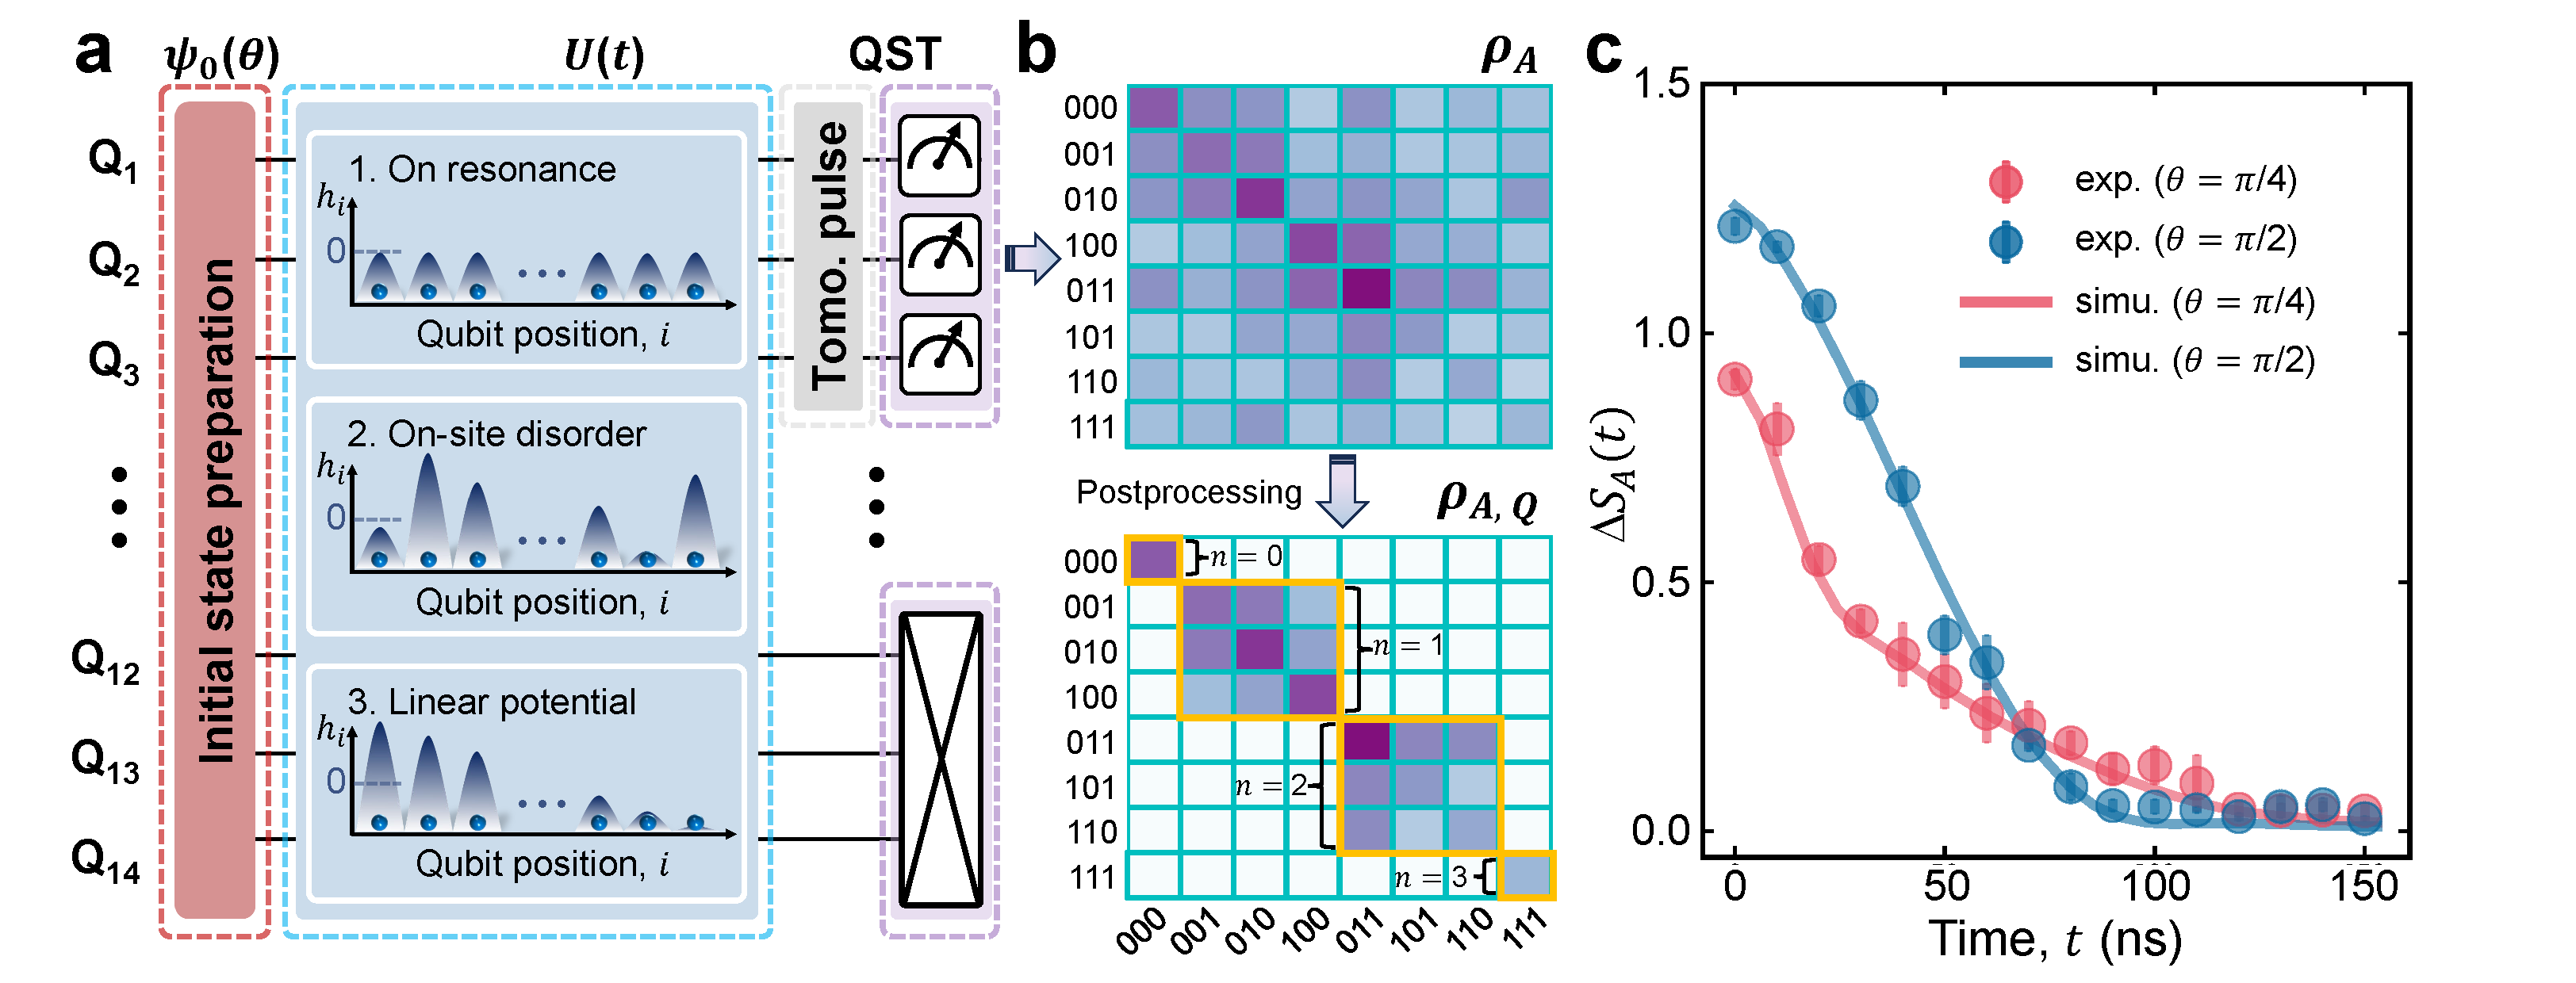
\includegraphics[width=1.0\linewidth]{Figure2/Figure2.pdf}
     	\caption{\textbf{Experimental protocol for measuring the EA and its dynamics in strong short-range coupling regime ($ r \approx 10 $).} \textbf{a}, Quantum circuit of experimental protocol. After initial state preparation of $ \ket{\Psi(\theta)} $, the system evolves under the engineered Hamiltonian \( H \) as $\ket{\Psi(t)}= U(t) \ket{\Psi(\theta)}=e^{-iHt} \ket{\Psi(\theta)}$, which involves different types of on-site potentials (resonance, disorder, or linear gradient field) applied to the qubits. \textbf{b}, The density matrix of subsystem $A$ reconstructed via QST. Following projection of the density matrix onto the eigenspaces of the charge operator $ Q_A $, classical post-processing is applied to estimate the EA. \textbf{c}, EA dynamics under strong short-range coupling regime ($ r \approx 10 $) with qubits on resonance, for tilted Néel initial states with angles $\theta = \pi/4$ and $\pi/2$. Faster symmetry restoration is observed for $\theta = \pi/2$ and an obvious crossover is observed, confirming the presence of QME. Symbols are experimental data and solid curves represent the theoretical results including decoherence (see Supplementary Information Note 4 for more details). Error bars represent the standard deviation obtained from 10 experimental repetitions, each comprising 3000 shots.
     	}

	\label{fig2}
     \end{figure*}
    
    To explore the QME, we prepare tilted product states that break global $ U(1) $ symmetry by an angle $ \theta $, with qubit idle frequencies optimized for high-fidelity initial state preparation and minimal microwave crosstalk~\cite{supp_cite}.
    The system is then subjected to a sudden quench under the engineered Hamiltonian \( H \), which incorporates tunable on-site potentials (resonance, disorder, or linear potentials) applied to the qubits (see Fig.~\ref{fig2}\textbf{a}). To investigate the dynamics of EA, we reconstruct the reduced density matrix \( \rho_A(t) \) of the subsystem \( A = \{Q_1, Q_2, Q_3\} \) using quantum state tomography (QST), and compute its projection \( \rho_{A,Q}(t) \) onto the eigenspaces of the charge operator \( Q_A = \sum_{i \in A} \sigma_i^z\) (see Fig.~\ref{fig2}\textbf{b}). Through the analysis of EA dynamics using Eq.~\eqref{EA}, we quantify the relaxation rates of states with different initial symmetry-breaking.
    
   
	~\\
	\textbf{\textbf{QME in strong short-range coupling regime}}
	
    We initially explore the dynamics of EA in the strong short-range coupling regime ($ r \approx 10 $), exploiting the tunable coupling strengths of our system. The nearest-neighbor couplings are fixed at $ g_N/2\pi = -5 \, \text{MHz} $, while long-range interactions yield an average coupling $ g_L/2\pi \approx 0.5 \, \text{MHz} $~\cite{supp_cite}, facilitating an approximate mapping to an integrable one-dimensional  XX  spin chain with open boundaries during early-time dynamics.

    The initial states are prepared as tilted Néel states, denoted  $ \ket{\theta}_N $, with different tilt angles $ \theta=\pi/4 $ and $ \theta = \pi/2 $, constructed by applying a Y-rotation of angle $ \theta $ to each qubit. The state can expressed as \( \ket{\theta}_N = \bigotimes_{j=1}^{14} R_y(\theta) \ket{s_j} \), where \( \ket{s_j} = \ket{0} \) ($\ket{1}$) for odd (even) \( j \), and the Y-rotation operator is defined as \( R_y(\theta) = e^{-i \theta \sigma_y / 2} \). The tilt angle \( \theta \) governs the degree of global \( U(1) \) symmetry breaking: in the Bloch sphere representation, \(\theta=0\) or \(\pi\) yields all spins aligned along \( \sigma_z\)-direction (fully symmetric), whereas \(\theta=\pi/2\) aligns all spins along \(\sigma_x\) (maximal symmetry breaking), indicating \( \ket{\theta= \pi/2}_N \) exhibits greater initial symmetry breaking compared to \( \ket{\theta= \pi/4}_N \).
    
    Following state preparation, we modulate the system to the target Hamiltonian $ H $ with all qubits tuned to resonance at $\omega_{\mathrm{ref}}/2\pi \approx 4.24 \, \text{GHz}$, and track the EA dynamics for a terminal subsystem $A$. As depicted in Fig.~\ref{fig2}\textbf{c}, despite the EA for $ \ket{\theta= \pi/2}_N $ initially exceeding that of $ \ket{\theta= \pi/4}_N $, the faster symmetry restoration of $ \ket{\theta= \pi/2}_N $ results in a more rapid decay rate, yielding a pronounced crossover phenomenon—a hallmark of the QME. Furthermore, our simulation results reveal the emergence of QME in a broad coupling regime (\( 1/r \leq 0.15 \))~\cite{supp_cite}. This effect originates from quasiparticle-mediated relaxation~\cite{Integrable_PRL,quasiparticle,integrable_arxiv}, wherein entangled quasiparticle pairs generated within subsystem $ A $ govern $ \Delta S_A $, with larger tilt angles $ \theta $ preferentially exciting faster-propagating modes, thereby accelerating symmetry restoration. 

	~\\
	\textbf{\textbf{QME suppression in intermediate coupling regime}}

     \begin{figure*}[t]
         \centering
     	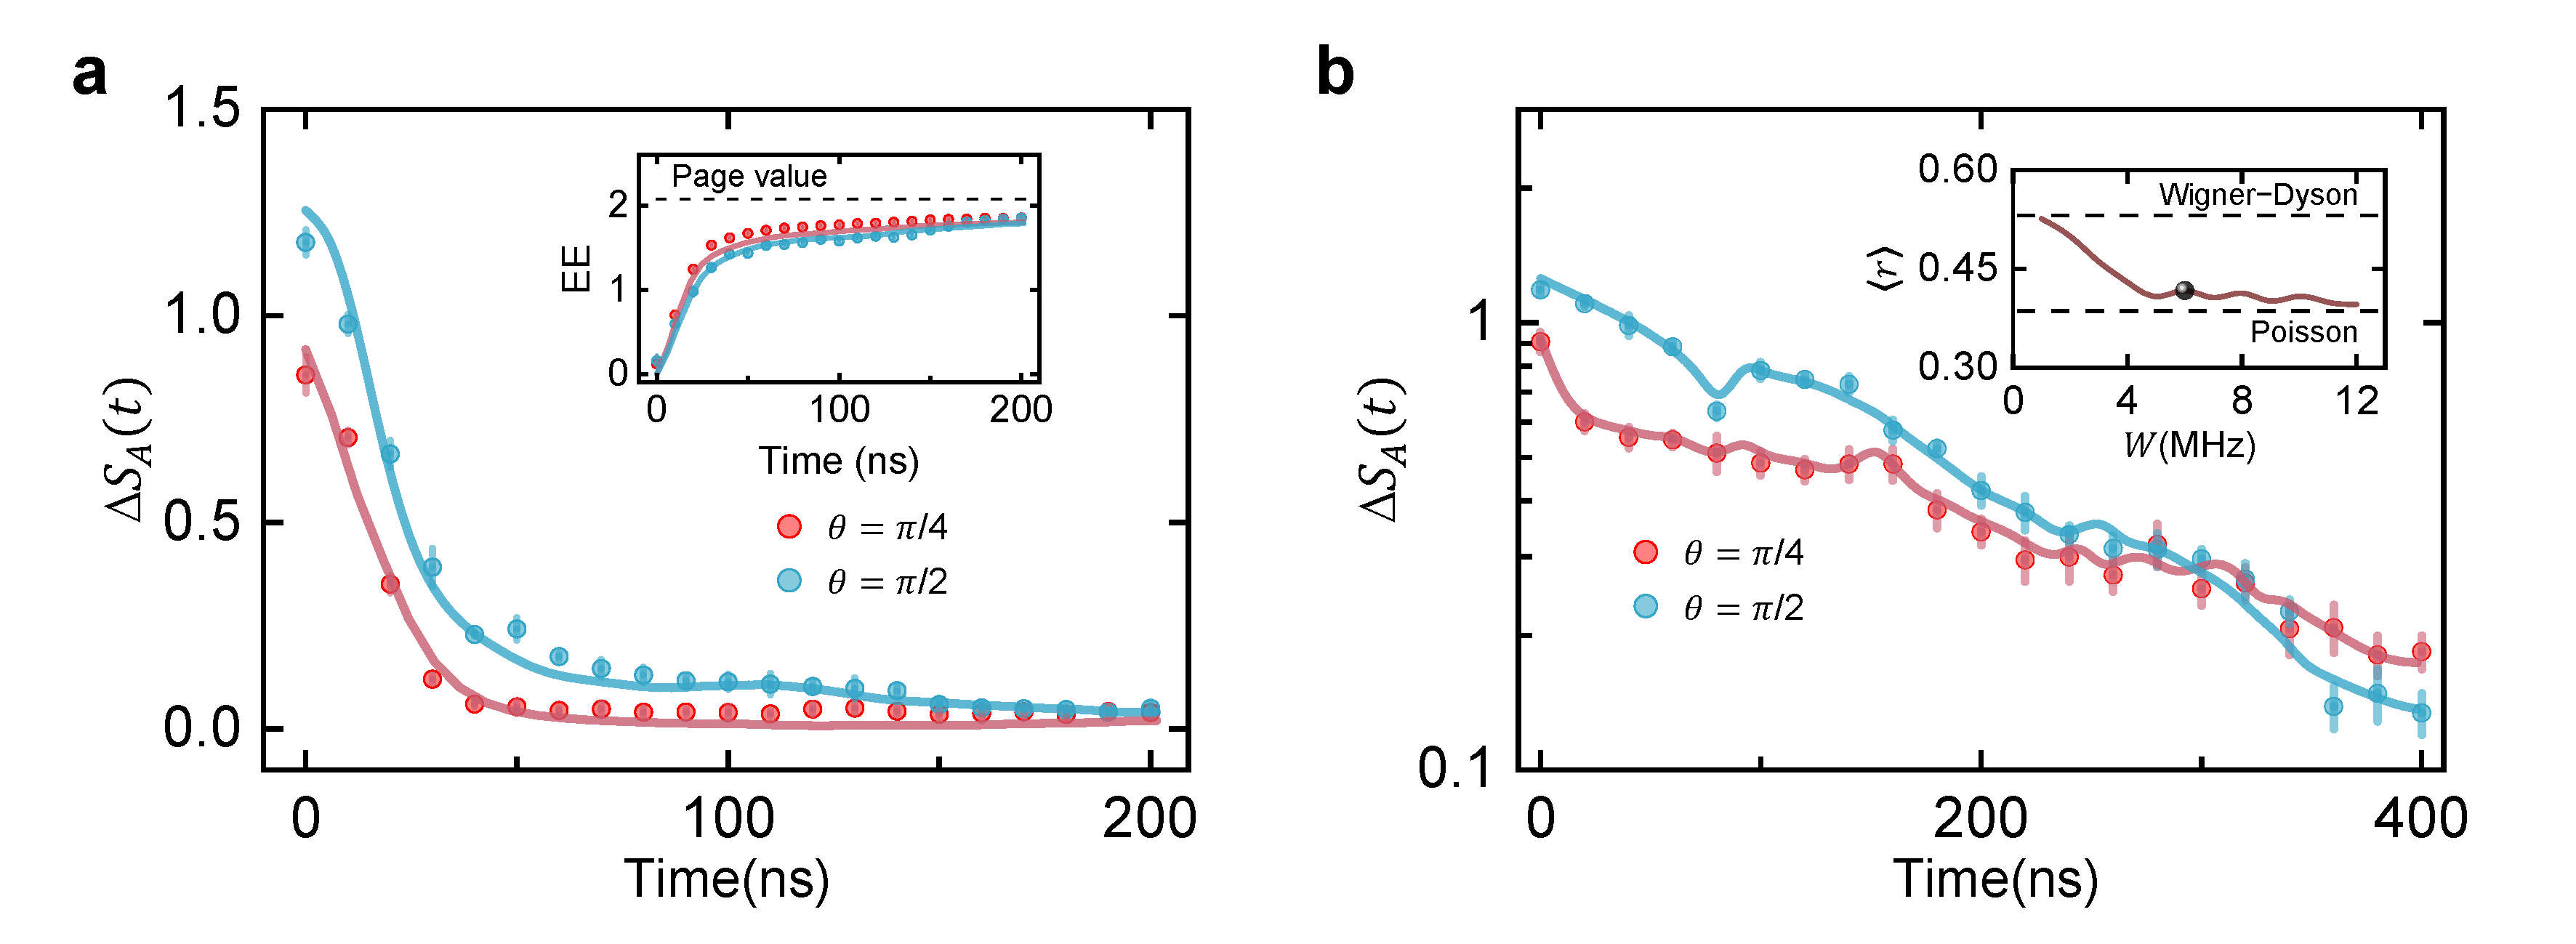
\includegraphics[width=1.0\linewidth]{Figure3/Figure3.pdf}
     	\caption{\textbf{EA dynamics in the intermediate coupling regime ($ r \approx 1 $) with tilted Néel states.} \textbf{a}, EA dynamics for tilted Néel states with angles \(\theta = \pi/4\) and \(\pi/2\) with qubits on resonance. Slower symmetry restoration for $\theta = \pi/2$, resulting in the disappearance of the dynamical crossover, indicating the suppression of QME. The inset shows that the entanglement entropy (EE) approaches the Page value as time increases.
     	\textbf{b}, Average ratio of consecutive level spacings \(\langle r \rangle\) as a function of linear potential strength \( W \) for a system size with \( N = 14 \) in the inset. As \( W \) increases, \(\langle r \rangle\) decreases from 0.53 to 0.39. EA dynamics for tilted Néel states with angles \(\theta = \pi/4\) and \(\pi/2\) in the presence of on-site potentials with \( W = 6 \, \text{MHz} \). Faster symmetry restoration for $\theta = \pi/2$, confirming the reemergence of QME. Symbols represent the experimental data, and solid curves denote theoretical results with decoherence. Error bars indicate the standard deviation from 10 experimental repetitions.}

	\label{fig3}
     \end{figure*}

    A primary experimental challenge lies in achieving precise control over the system Hamiltonian to investigate the sensitivity of QME to thermalization processes. We address this challenge in the intermediate coupling regime (\( r \approx 1 \)), where the nearest-neighbor coupling strength is set to \( g_N/2\pi = -2 \, \text{MHz} \) and the long-range interaction strength \( g_L/2\pi \) is tuned around \(-2 \, \text{MHz}\)~\cite{supp_cite}. In this configuration, we prepare the same tilted initial states as in the \(r\approx10\) case. Here, thermalization governs the system dynamics, driving the subsystem towards thermal Gibbs ensembles—a process inherently linked to $ U(1) $ symmetry restoration in the Hamiltonian $ H $.
    
    Figure~\ref{fig3}\textbf{a} displays the EA dynamics for subsystem \(A\), revealing a key departure from the strong short-range regime: states with greater initial symmetry breaking exhibit slower symmetry restoration compared to those with less breaking. Therefore, the dynamical crossover vanishes, resulting in the suppression of QME. Prior studies revealed a positive correlation between the speed of symmetry restoration and the thermalization rate~\cite{random_circuits_2024}, characterized by the entanglement entropy (EE). To investigate the relationship experimentally, we compute the EE through the von Neumann entropy derived from reduced density matrices, as shown in the inset of Fig.~\ref{fig3}\textbf{a}. 
    The EE for both initial states increases linearly before saturating and approaches the Page value, signaling thermalization. Moreover, EA exhibits an initial near-linear decrease, subsequently approaching zero gradually, mirroring the dynamical evolution of the EE. 
    % The EE increases linearly before saturating, while EA exhibits an initial near-linear decrease, subsequently approaching zero gradually, mirroring the dynamics of the EE.
    Meanwhile, the state with a smaller tilt angle exhibits faster entropy growth---characteristic of accelerated thermalization---which suppresses the emergence of QME. Therefore, our findings not only demonstrate that flexible modulation of coupling configuration enables the tunable manipulation of QME, but also elucidate an intimate link between the restoration of system symmetry and thermalization dynamics.
    	
	~\\
	\textbf{\textbf{Reemergence of QME}}

    Building on the aforementioned insights, an intriguing question arises: can we leverage the flexibility of our system-such as varied on-site potentials and diverse initial states-to recover QME in the intermediate-coupling regime? Previous theoretical studies have shown that the suppression of thermalization and the breakdown of ergodicity lead to the emergence of QME for arbitrary tilted product states~\cite{QME_MBL}. 
    
    Inspired by these findings, we introduce the position-dependent on-site potential \(h_j/2\pi = W(7.5-j)\) for qubit \(Q_j\) with \(j = 1, 2, \ldots, 14\), to break the ergodicity of system. To quantify the suppression of ergodicity, we compute the average level-spacing ratio \(\langle r \rangle\), defined as~\cite{2013_PRL_Level_Ratio} 
    \begin{equation}
    \expval{r} = \frac{1}{N} \sum_{n=1}^N \frac{\min(\delta_n, \delta_{n+1})}{\max(\delta_n, \delta_{n+1})}
    \end{equation}
    with \(\delta_n = E_{n} - E_{n-1} > 0 \) being the difference between the \(n\)th and \((n-1)\)-th eigenenergy of the Hamiltonian Eq.~\eqref{hamiltonian}. The ergodic phase is characterized by Wigner-Dyson level-spacing statistics (\(\langle r \rangle \approx\) 0.531), while the localized phase exhibits Poisson statistics (\(\langle r \rangle \approx\) 0.386)~\cite{2019_PNAS_mbl,2020_PRB_mbl}. In our system, as \(W\) increases, \(\langle r \rangle \) approaches 0.386 (see the inset of Fig.~\ref{fig3}\textbf{b}), signifying suppressed ergodicity and emergent localization-like features within experimentally accessible finite-size regimes.
    
    The EA dynamics for \(W = 6 \, \text{MHz}\) in Fig.~\ref{fig3}\textbf{b}, revealing key distinctions from the on-resonance case (\(W = 0 \, \text{MHz}\)): symmetry restoration slows with increasing \(W\). Meanwhile, the suppression of symmetry restoration exhibits tilt-angle dependence, with larger angles $\theta$ showing weaker suppression, thereby regenerating a dynamical crossover that recovers QME. Long-time EA simulations within the accessible \(W\) range corroborate this mechanism~\cite{supp_cite}: as \(W\) increases, the late-time EA of \( \ket{\theta = \pi/4}_N \) rises while \( \ket{\theta = \pi/2}_N \) remains nearly constant. This phenomenon results in $\Delta S_A(\pi/4,t\to \infty)>\Delta S_A(\pi/2,t\to \infty)$, guaranteeing crossover emergence in our experimental regimes.

     \begin{figure*}[t]
         \centering
     	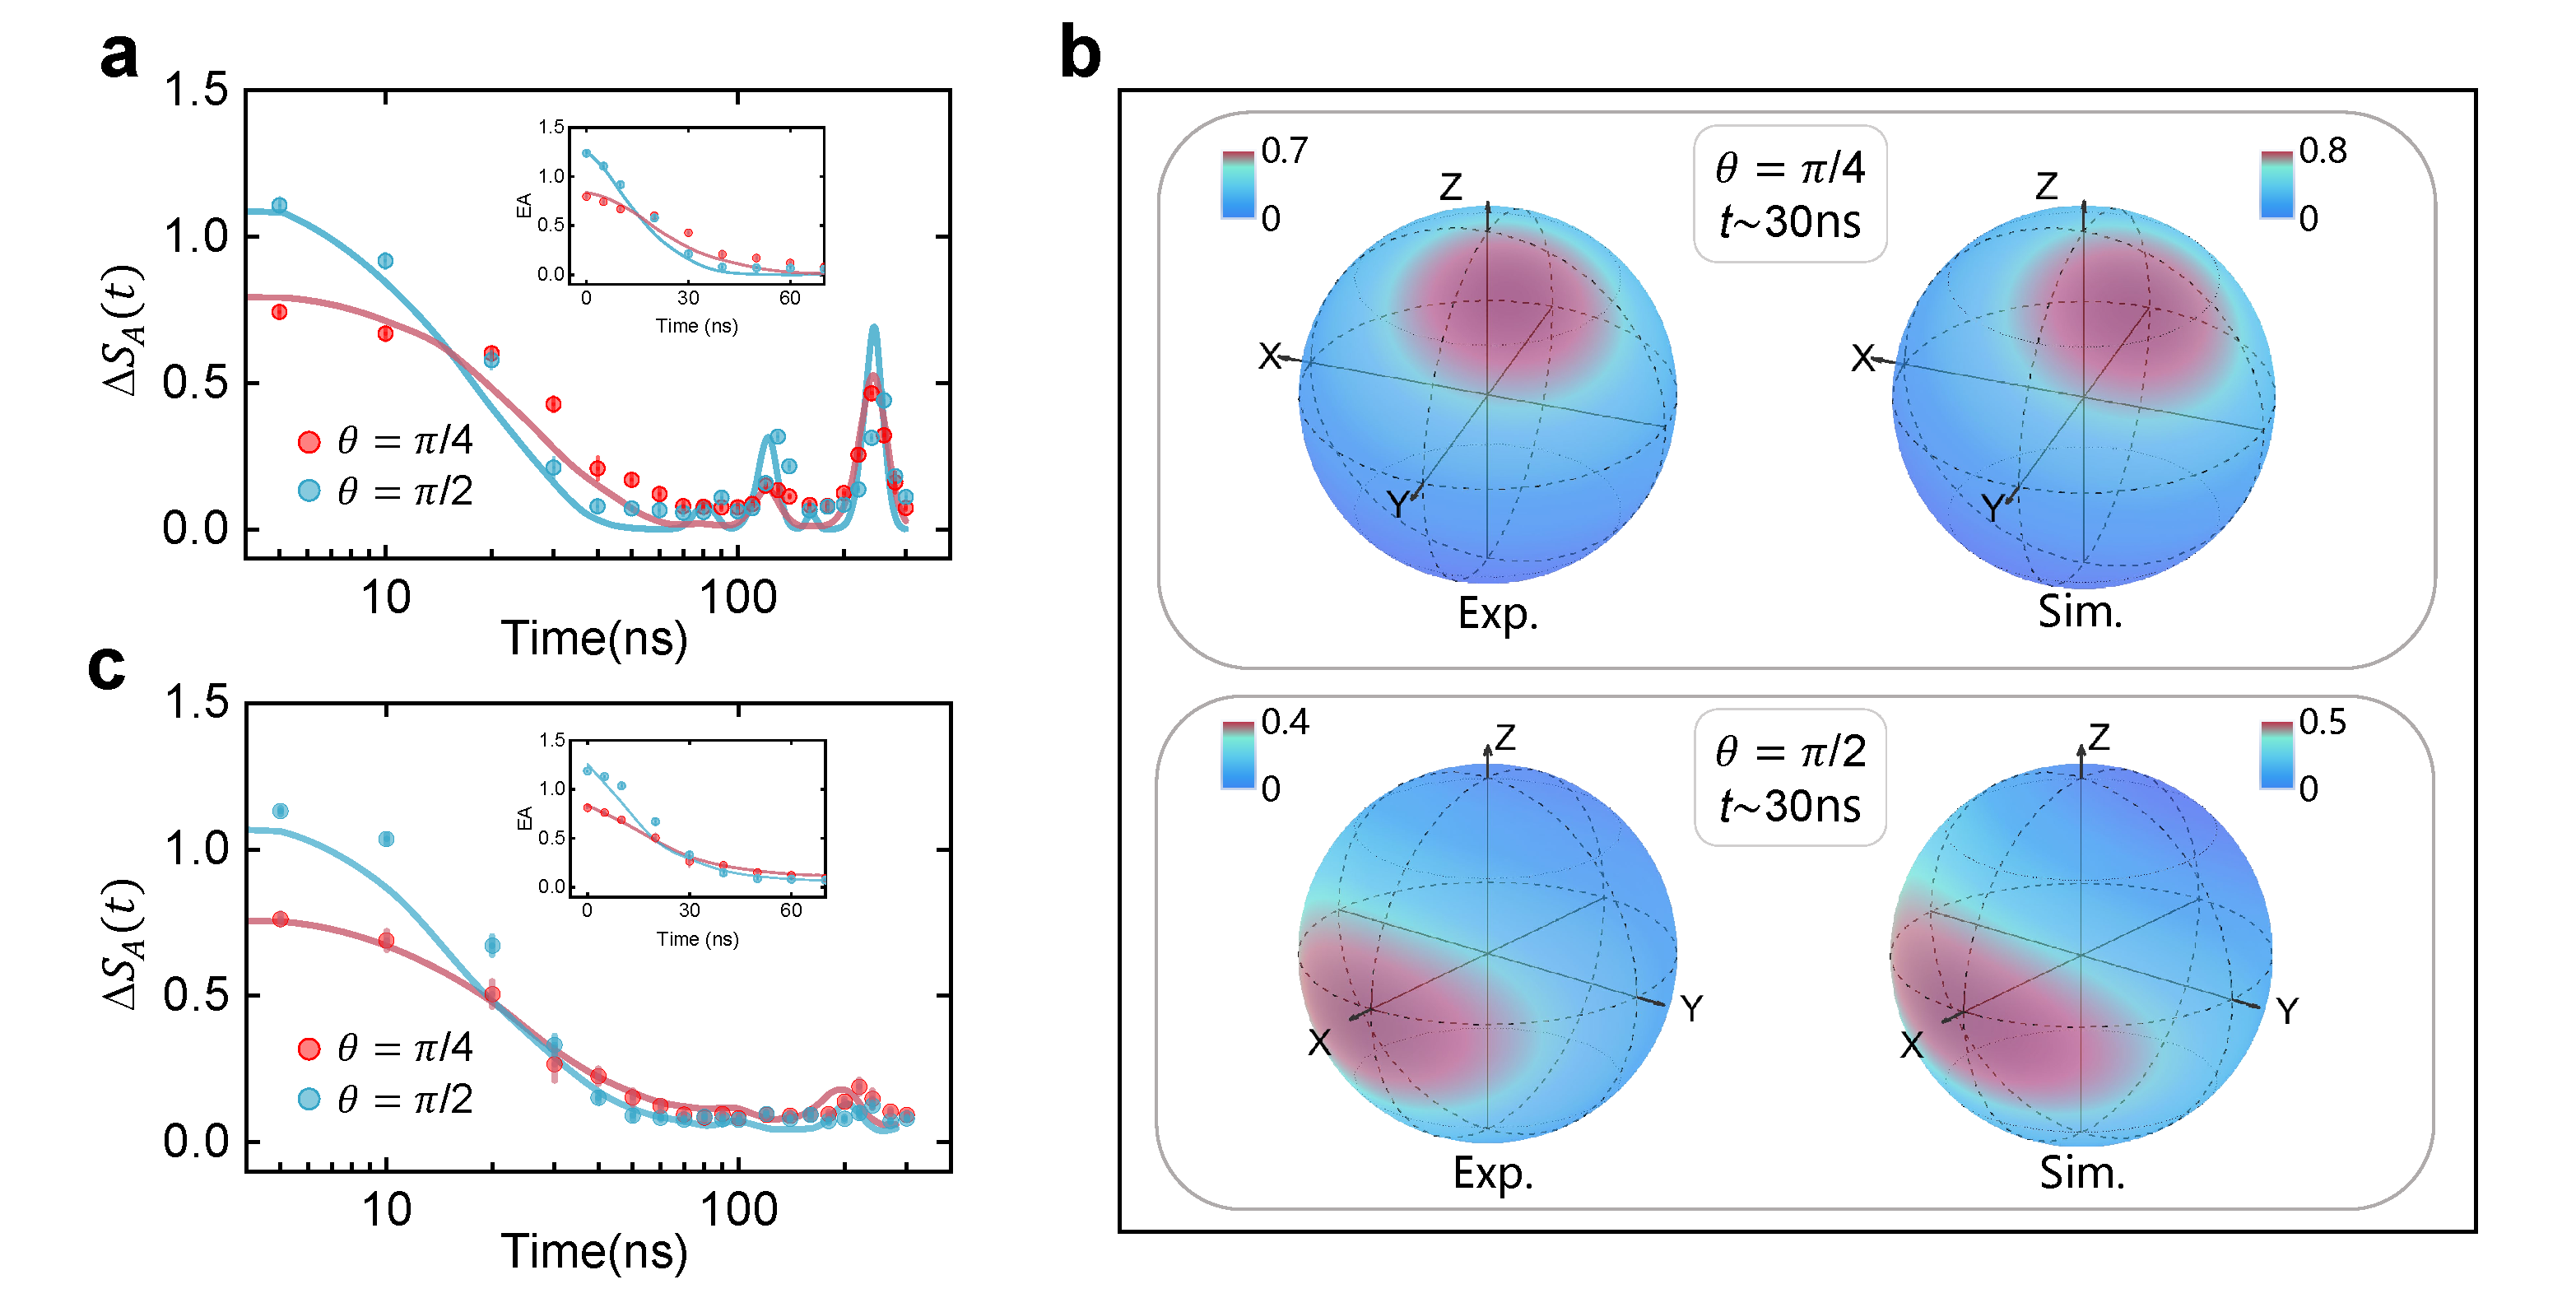
\includegraphics[width=1.0\linewidth]{Figure4/Figure4.pdf}
     	\caption{\textbf{EA dynamics in the intermediate coupling regime ($ r \approx 1 $) with tilted ferromagnetic states.} \textbf{a}, EA dynamics for tilted ferromagnetic states at angles \(\theta = \pi/4\) and \(\pi/2\) with qubits on resonance. The EA exhibits a clear crossover accompanied by oscillations as a function of interaction time. The inset shows EA dynamics with a linear time axis. Numerical simulations with decoherence are shown as solid lines, and experimental data are points. Error bars indicate the standard deviation of the experimental data. \textbf{b}, Experimental and numerical data of quasidistribution function in spherical coordinates with evolution time \(t~\approx30\) ns for \(\theta = \pi/4\) and \(\pi/2\), respectively. \textbf{c},	EA dynamics for tilted ferromagnetic states with two tilt angles in the presence of on-site disorder, sampled from a uniform distribution \( [-14\bar{g}, 14\bar{g}] \). Data points denote experimental results with 6 disorder realizations, while solid lines represent theoretical results without decoherence averaged over 100 disorder realizations. Error bars indicate the standard error of the experimental results.}

	\label{fig4}
     \end{figure*}

    An alternative strategy to recover the QME is to quench from tilted ferromagnetic states in the intermediate-coupling regime (\( r \approx 1 \)). In this case, the early-time dynamics can be mapped onto the LMG model. This mapping is facilitated by introducing the collective spin operators \( \boldsymbol{S} = \sum_i \boldsymbol{\sigma}^i / 2 \), leading to the Hamiltonian:
    \begin{equation}
        \begin{aligned}
        H &= \sum_{i< j} \bar{g} (\sigma_i^+ \sigma_j^- + \sigma_i^- \sigma_j^+ ) \\
        &\approx \bar{g}(\boldsymbol{S}^2 - S_z^2),
        \end{aligned} 
    \end{equation}  
    where $\bar{g}$ denotes the average coupling strength (\(\bar{g}/2\pi \approx -2 \, \text{MHz}\)). The tilted ferromagnetic states \( |\theta\rangle_F \) are expressed in the collective spin basis \(|S, S_z\rangle\), and possess maximal total spin quantum number \(S = N/2\), with \( N \) being the total particle number of the system. 
    Since $\boldsymbol{S}^2$ is conserved, the effective Hamiltonian reduces to the LMG model \(H_{\text{eff}} = -\bar{g} S_z^2\), a paradigmatic system for studying dynamical phase transitions and many-body entanglement~\cite{2020_SA_xu}.

    Figure~\ref{fig4}\textbf{a} shows the EA dynamics quenched from tilted ferromagnetic states with $\theta = \pi/4$ and $\pi/2$, respectively. Notably, increased tilt angle $\theta$ enhances early-time symmetry restoration, thereby recovering QME with an obvious crossover. The subsystem dynamics are confined to the $S_A = N_A/2$ subspace, leading to the time-independence of the projected density matrix $\rho_{A,Q}$.
    This directly yields \(\Delta S_A(\theta,t) = C(\theta) - S_A(\theta,t)\), with $C(\theta)$ as an initial-state-dependent constant~\cite{supp_cite}. Therefore, the symmetry restoration rate precisely tracks the growth rate of EE, while the monotonic $\theta$-dependence of both $C(\theta)$ and $\partial_t S_A(\theta,t)$ dictates the crossover of EA. For the ideal LMG model, we derive exact solutions for the EA dynamics, further exploring the relationship among the crossover behavior, entropy type, and system size \cite{supp_cite}.

    Although the LMG model is exactly solvable, its symmetry restoration dynamics cannot be explained by quasiparticle propagation. Instead, the process is best visualized through the quasidistribution function $Q(\theta,\phi) = \langle \theta,\phi | \rho_A | \theta,\phi \rangle$, where $|\theta,\phi\rangle$ represents a coherent spin state~\cite{2019_science}.
    The dynamical flattening of the azimuthal ($\phi$-direction) distribution directly reflects the restoration of $U(1)$ rotational symmetry. As demonstrated in Fig.~\ref{fig4}\textbf{b}, the distribution for $\theta = \pi/2$ exhibits faster flattening compared to $\theta = \pi/4$, providing a clear signature of the QME in the early-time dynamics. In addition, recent studies employing time-dependent spin wave analysis show that $\Delta S_A$ directly corresponds to semi-classical spin fluctuations in the azimuthal direction~\cite{QME_long_range_spin}, which agrees well with the $Q$-function description of the dynamics. Furthermore, the collective spin dynamics display characteristic periodic behavior: the EA oscillates with period $T_{\text{EA}} = \pi/\bar{g}$, while the full revival occurs at $T_S = 2\pi/\bar{g}$. This exact relationship $T_S = 2T_{\text{EA}}$ originates from the symmetry equivalence $|\psi(T_S/2)\rangle \propto |{-}\theta\rangle_F = R_z(\pi) |\theta\rangle_F$~\cite{supp_cite}. 

    To suppress oscillations and unambiguously demonstrate the QME, we investigate the effect of on-site disorder on EA dynamics. Figure~\ref{fig4}\textbf{c} shows that the EA crossover persists under disorder \( h_i/2\pi \), sampled from a uniform distribution \( [-14\bar{g}, 14\bar{g}] \). The disorder breaks spin equivalence, eliminating collective behavior and periodic revivals. Although disorder slows relaxation, slightly prolonging the EA crossover time, the QME remains observable. Our observation of QME with strong disorder demonstrates its robustness for tilted ferromagnetic initial states in the intermediate-coupling regime (\( r \approx 1 \)). Previous studies of power-law XX spin chains have reported that the crossover disappears within the experimental timescales under comparable disorder strengths~\cite{QME_trapped_ion}. These studies considered the Hamiltonian in Eq.~\eqref{hamiltonian} with \( g_{ij} = g_0 / |i - j|^\alpha \), where \( g_0 \) is a constant and \( \alpha \approx 1 \). In contrast, for \( r = 1 \), the Hamiltonian corresponds to a power-law XX spin chain with exponent \( \alpha = 0 \), exhibiting stronger long-range interactions than the \( \alpha \approx 1 \) case. Our results reveal that stronger long-range interactions facilitate symmetry restoration, leading to more rapid EA crossovers within the experimental timescale.
 

    ~\\
	\textbf{Conclusion and outlook}
	
	In summary, we report the first experimental realization of multidimensional modulation of the QME within an isolated quantum system, achieved using a 16-qubit superconducting quantum circuit. The quantum processor features a fully connected architecture with tunable coupling, enabling flexible engineering of Hamiltonian parameters. Our study traces the QME emergence, suppression, and resurgence, providing a comprehensive framework for its control. In the near-integrable short-range limit (\( r \approx 10 \)), we observe the QME through an EA crossover with the tilted initial Néel states, which is driven by faster-propagating quasiparticle modes at larger tilt angles. In contrast, in the intermediate coupling regime (\( r \approx 1 \)), thermalization suppresses the QME, as reflected in the EA dynamics, which mirror the growth of entanglement entropy. Remarkably, QME reemerges through two distinct mechanisms: the introduction of an on-site linear potential, which induces localization-like behavior and modulates symmetry restoration rates in a tilt-angle-dependent manner, and quenches from tilted ferromagnetic states, which exhibit robust EA crossovers under strong on-site disorder.
    
    Looking ahead, our work establishes the QME as a general and controllable feature of non-equilibrium quantum dynamics, with potential applications in quantum  information. For instance, the modulation of QME enables controlled thermalization through accelerated equilibration, offering potential for efficient state preparation. Future investigations could explore QME in prethermalization regimes~\cite{2025_periodicallydrivenEA,prether_IME_arxiv} or under alternative symmetries, such as \( \mathbb{Z}_2 \) and \( SU(2) \), revealing deeper insights into this phenomenon. Furthermore, probing EA dynamics under symmetry-breaking Hamiltonians presents an intriguing avenue to deepen our understanding of the interplay between symmetry and thermalization~\cite{2025_QME_no_sym,Breaking_Hamitonion_zhang}. These explorations may advance applications of QME in quantum simulation and quantum information processing.
    \\
	

	
	\bibliography{main.bib}
	
	~\\
	\noindent
	\textbf{Acknowledgements}\\
	We thank Zheng-Hang Sun for helpful discussions. This work was supported by National Natural Science Foundation of China (Grants Nos.~12447184, 12404578, 92265207, 92476202, 92365301, T2121001, 12204528, T2322030, 12247168), Innovation Program for Quantum Science and Technology (Grant No.~2021ZD0301800), Beijing Nova Program (Nos.~20220484121, 20240484652) and Beijing National Laboratory for Condensed Matter Physics (2024BNLCMPKF022). The device used in this work was made at the Nanofabrication Facilities at Institute of Physics, CAS in Beijing.
	
	~\\
    \noindent
    \textbf{Author contributions}\\
    H.F. and K.X., and K.H. supervised the project; C.-P.F. and Z.-Y.G. proposed the theoretical idea while H.F., K.X., Y.X., Y.-R.Z., K.H. and Y.-H.S. discussed and designed the experiment; M.-C.W. and B.-J.C. designed the quantum device and B.-J.C. fabricated it with the help of G.-H.L. and X.S.; Y.X. performed the experiment with the assistance of K.X., K.H., and Y.-H.S.; Y.X. and C.-P.F analyzed the experimental data with the assistance of S.-X.Z., Z.-Y.G. and H.F.; Y.-H.S., Y.L., C.-L.D, K.Z., Z.-H.L. and T.-M.L. contributed to the discussion on experimental parameter optimization and analysis; C.-P.F and Y.X. performed the numerical simulations; S.-X.Z., C.-P.F and Z.-Y.G. gave theoretical explanations; Y.-H.S., T.-M.L. and J.-C.Z. contributed to the waveform distortion correction; K.H., K.Z., H.L., Z.W., C.-L.D. and H.-T.L. helped with the experimental setup; Y.X., C.-P.F, K.H., M.-C.W., B.-J.C., K.X., and H.F. co-wrote the manuscript, and all authors contributed to the discussions of the results and development of the manuscript.

    ~\\
    \noindent
	\textbf{\textbf{Competing interests}}\\
	The authors declare no competing interests.


	\vspace{-1mm}
	
	
	
\clearpage 
\onecolumngrid
\begin{center}
{\large \bf Supplementary Information for:\\ Observation and Modulation of the Quantum Mpemba Effect on a Superconducting Quantum Processor}
\\
\vspace{0.3cm}
\end{center}

\vspace{0.6cm}
%\twocolumngrid


\beginsupplement
\makeatletter
\def\@hangfrom@section#1#2#3{\@hangfrom{#1#2#3}}
\makeatother

\setcounter{section}{0}
\renewcommand{\thesection}{Supplementary Note \arabic{section}}
\renewcommand{\figurename}{Supplementary Fig.}
\setcounter{figure}{0}  % reset counter
% \renewcommand{\thetable}{Supplementary Table \arabic{table}}
% \setcounter{table}{0}  % reset counter

\renewcommand{\tablename}{Supplementary Table}
\setcounter{table}{0}
\renewcommand {\thetable} {\arabic{table}}%
\tableofcontents

    \section{Experimental device and performance}
    
    The architecture of our superconducting quantum processor consists of 16 frequency-tunable transmon qubits arranged in a ring, capacitively coupled to a central frequency-tunable bus resonator. Each qubit is also connected to its two nearest neighbors via flux-tunable couplers. The chip is fabricated using the flip-chip recipe and its layout was systematically optimized to minimize unwanted coupling and microwave crosstalk, as shown in Supplementary Fig.~\ref{chip}. The central bus, a \(\lambda/2\) superconducting aluminum stripline resonator, is designed to mediate global interactions across the processor. To maintain signal integrity, coplanar waveguide (CPW) resonators route microwave signals to each qubit. Furthermore, strategically placed ground plane cutouts and air-bridge crossovers were implemented to suppress spurious slot-line modes and ensure a consistent characteristic impedance across the chip. The superconducting quantum processor sample was placed in a domestically manufactured dilution refrigerator (CETC16, XS400), which exhibited a base temperature of 9 mK in the absence of thermal load and stabilized at 10 mK under experimental conditions following the integration of signal and control wiring.

    \begin{figure}
		\centering
		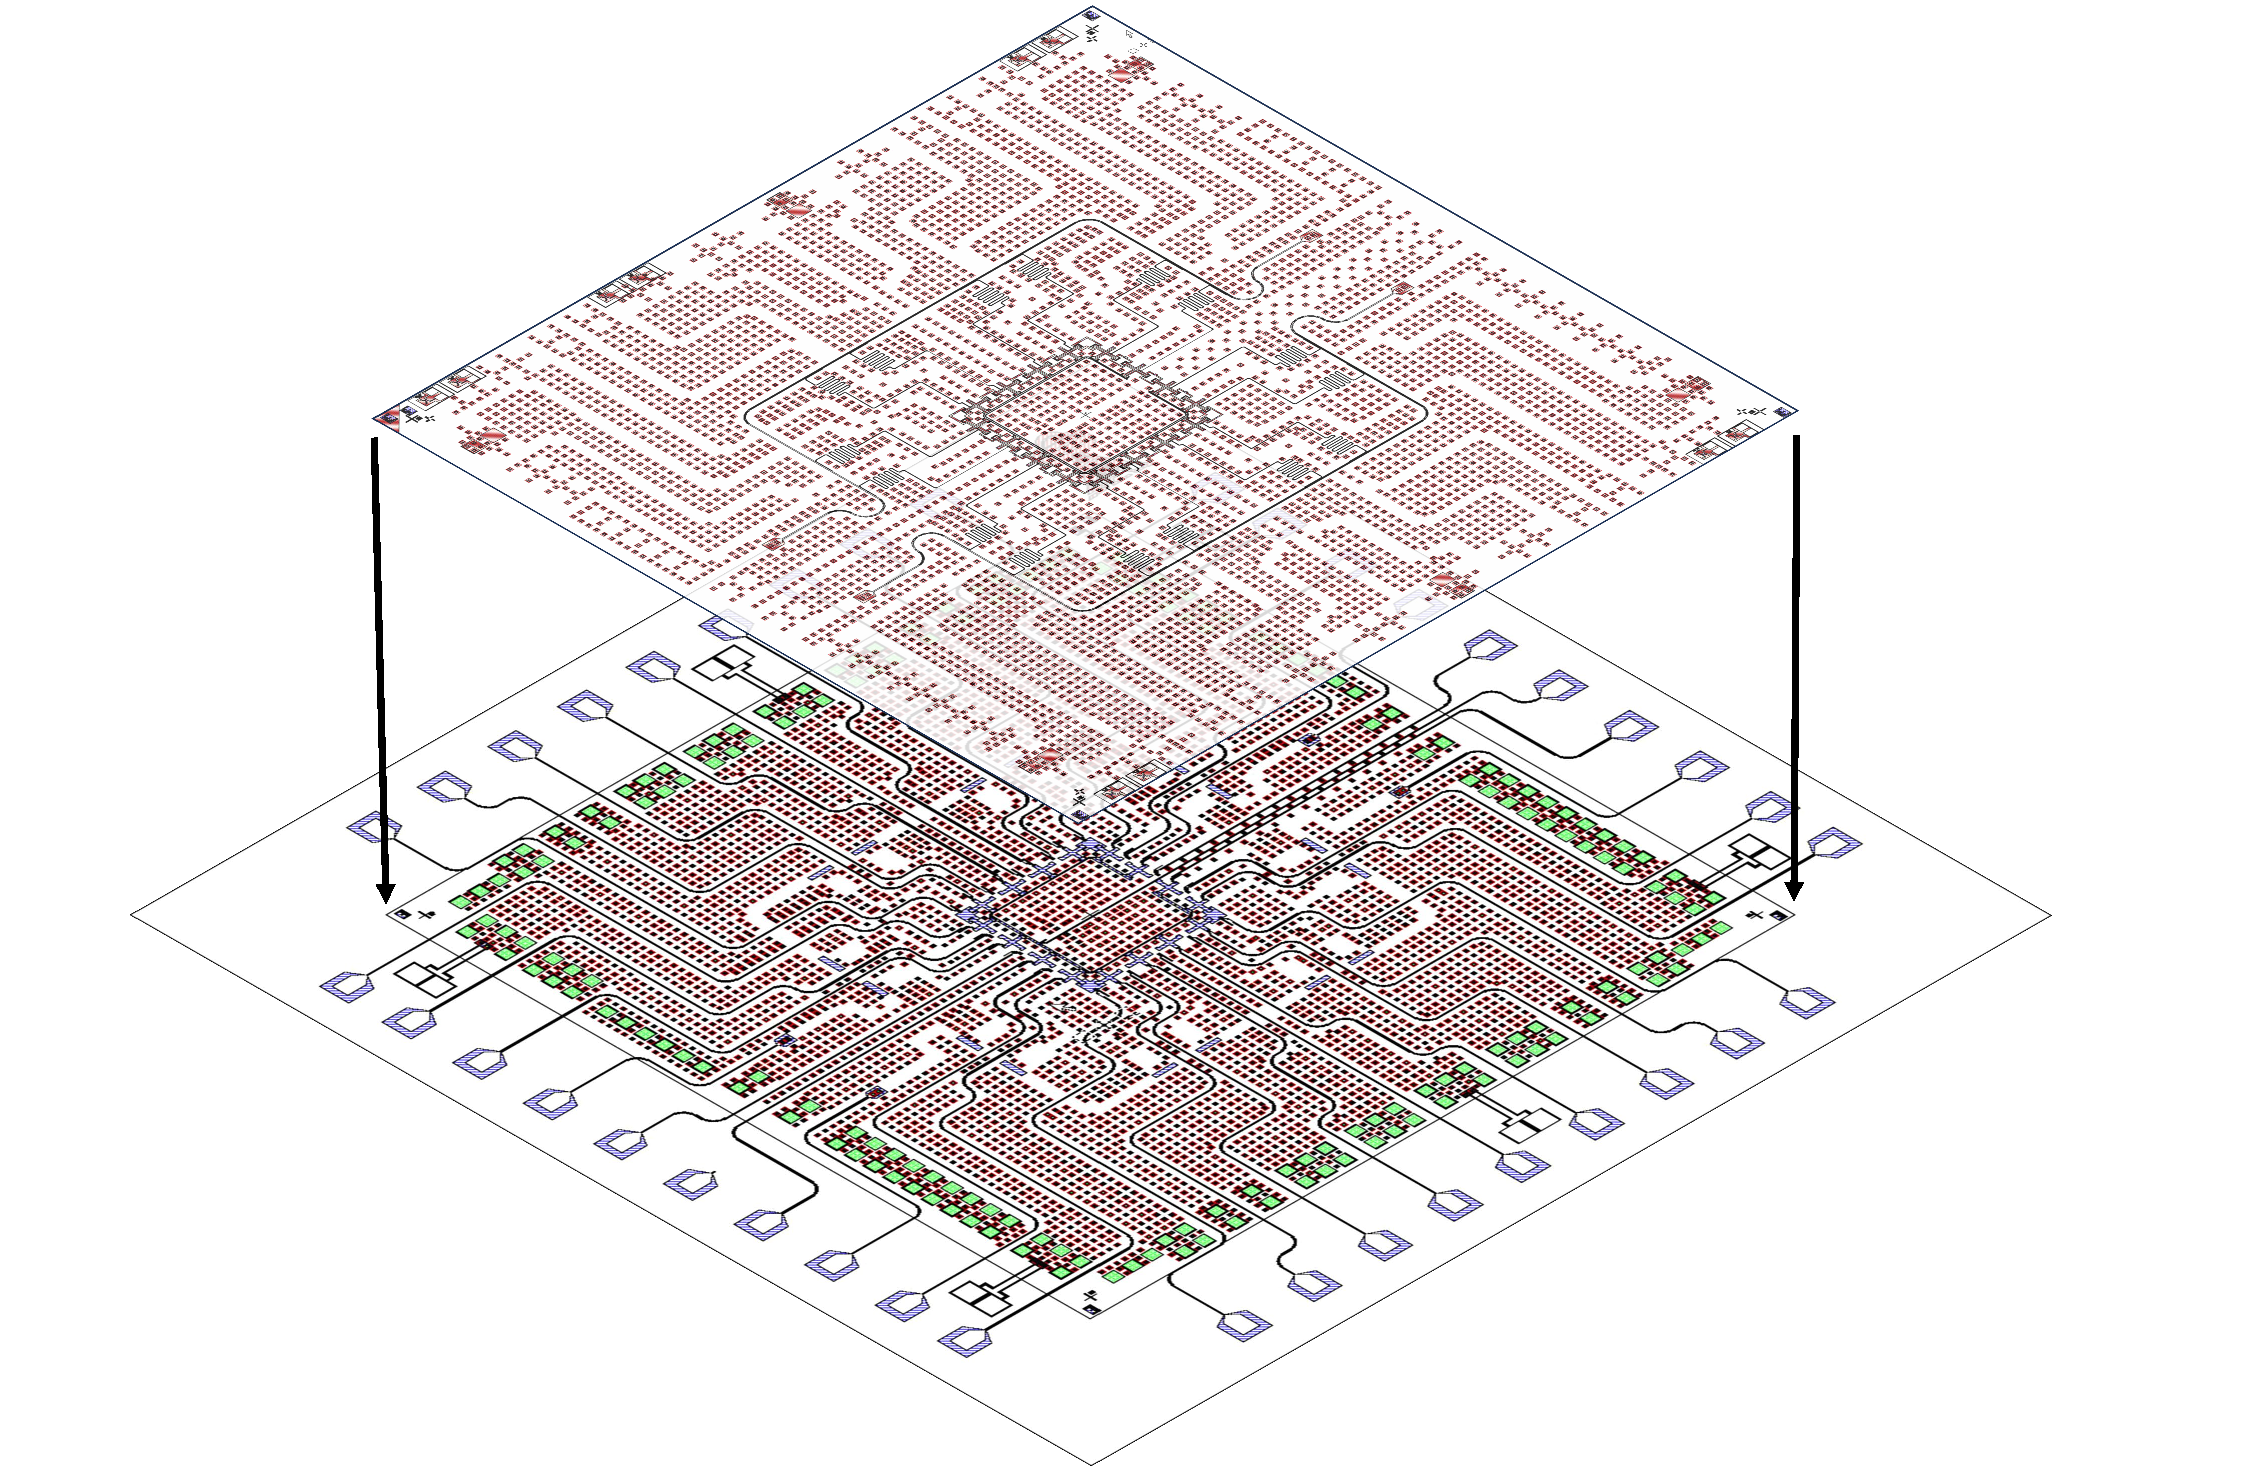
\includegraphics[width=1.0\linewidth]{suppFig/flip_chip.pdf}
		\caption{\textbf{The micrograph of the superconducting quantum processor employing a flip-chip architecture.}}
		\label{chip}
	\end{figure}
	
	\subsection{Device fabrication}
         

    The superconducting quantum chip was fabricated on a (0001)-orientation sapphire substrate using a multi-step process, culminating in a flip-chip bonding procedure to integrate the qubit and wiring layers. The detailed fabrication flow is as follows.
    
    \textbf{I. Substrate Preparation and Base Layer Deposition.}
    Two double-side polished sapphire wafers were first annealed. Subsequently, a 100 nm layer of aluminum (Al) was deposited on each wafer using electron beam evaporation. This was immediately followed by an \textit{in-situ} oxidation step to form a thin, dense layer of aluminum oxide ($AlO_x$). This oxide layer serves to protect the underlying aluminum film and ensure uniformity during subsequent etching processes.
   
      \textbf{II. Qubit and Wiring Layer Patterning.}
    The primary circuit patterns for the qubit layer and the wiring layer were defined on their respective wafers. The SPR-955 photoresist was spin-coated onto the wafer surfaces and patterned using laser direct writing (LDW). The exposed patterns were then developed using a Tetramethylammonium hydroxide (TMAH) solution. The aluminum was etched with a heated etchant, and the remaining photoresist was stripped using N-Methylpyrrolidone (NMP) to yield the final qubit and wiring wafers.
  
      \textbf{III. Niobium Interconnection and Alignment Marks.}
    A 100 nm niobium (Nb) layer was deposited to serve as a transition layer between the aluminum and indium, and as alignment marks for subsequent electron beam lithography. A bilayer resist of LOR-5A and SPR-955 was spin-coated, exposed, and developed to create a pattern with an undercut profile, ideal for a lift-off process. Prior to Nb deposition via magnetron sputtering, the native $AlO_x$ on the aluminum surface was removed with an \textit{in-situ} argon ion cleaning step. Finally, the photoresist was removed to lift off the excess niobium film.
  
    \textbf{IV. Josephson Junction Fabrication.}
    Josephson junctions were fabricated on the qubit wafer using electron beam lithography (EBL). A bilayer of MAA-EL9 and PMMA-A5 resist was spin-coated, followed by the deposition of a 10 nm Al layer to act as a charge dissipation layer. The junction pattern was exposed using multiple electron doses. After exposure, the conductive Al layer was removed, and the pattern was developed in a solution of methyl isobutyl ketone (MIBK) and isopropanol (IPA).
    The junctions were formed using a double-angle evaporation technique in an electron beam evaporator. An initial \textit{in-situ} argon ion clean removed the native oxide on the base aluminum layer. The first Al layer (65 nm) was evaporated, followed by a controlled \textit{in-situ} oxidation step to form the tunnel barrier. The second Al layer (100 nm) was then evaporated at a different angle. The resistance of the resulting junction, which determines its Josephson energy, was controlled by tuning the oxidation time and pressure. A final lift-off step in acetone removed the excess aluminum. The junction resistance was verified post-fabrication using a probe station to ensure it met design specifications.
  
    \textbf{V. Air-Bridge Fabrication.}
    To ensure robust grounding and suppress parasitic modes, air-bridges were fabricated on both the qubit and wiring wafers. First, SPR-220 photoresist was spin-coated and patterned to define the air-bridge pillars. A reflow process was performed by heating the photoresist to create an arched profile for the bridge span. Next, after an in-situ argon ion clean, 500 nm of aluminum was deposited via electron beam evaporation, followed by in-situ oxidation. A second lithography step using S-1813 photoresist was performed to protect the air-bridge structures, after which the surrounding aluminum was removed with a heated aluminum etchant (Type-D). The process was completed by cleaning the surface with a pure oxygen plasma etch and stripping the remaining resist.
  
    \textbf{VI. Indium Bump Deposition.}
    Indium bumps were fabricated for the mechanical and superconducting connection between the two chips. A thick AZ-4620 photoresist was first spin-coated and exposed to define an undercut region. Following a rehydration and degassing period, a second layer of S-1813 photoresist was spin-coated and exposed to define the bump opening, resulting in a deep undercut structure after development. After an in-situ argon ion clean, 7 µm of indium was deposited using thermal evaporation. A reactive ion etch using a mixture of argon and oxygen was used for final cleaning before a lift-off process removed the excess indium, leaving the defined indium bumps.
  
    \textbf{VII. Dicing, Assembly, and Packaging.}
    Finally, the wafers were prepared for dicing by spin-coating a protective layer of AZ-4620 photoresist. A dicing saw was used to cut the wafers into individual qubit chips (11 mm × 11 mm) and wiring chips (15 mm × 15 mm). After stripping the protective resist, the two chips were aligned and bonded using a flip-chip bonder. The assembled chip was then placed in a sample box and electrically connected using an ultrasonic wire bonder. All connections were verified with a multimeter before the device was cleared for low-temperature testing.
% \end{minipage}
	
	\subsection{Device performance}
    Supplementary Table~\ref{Tab1} presents the performance metrics of qubits, including energy relaxation time \( T_1 \), Ramsey dephasing time \( T_2^* \), idle frequency $\omega^{\mathrm{idle}}_{j}/2\pi$, and single-qubit gate fidelity. To accurately measure the effective \( T_1 \) and \( T_2^* \) during system evolution, these parameters are evaluated at the interaction frequency, with couplers and the central bus resonator tuned to their operational frequencies. For states preparation, tilted initial states are generated by applying single-qubit rotations \( R_y(\theta) \) to the initial state. Here, single-qubit rotations \( R_y(\theta) \) are implemented using \( R_x(\theta) \) with virtual \( R_z(\pi/2) \) gates. For example, the  Y/2 gate is achieved using X/2 gate combined with the virtual \( R_z(\pi/2) \) gate. The tilted ferromagnetic states \(\ket{\pi/4}^{\otimes N}\) and \(\ket{\pi/2}^{\otimes N}\) (with $N=14$) are prepared by applying \( R_y(\pi/4) \) and \( R_y(\pi/2) \) rotations, respectively. In addition, tilted Néel initial states \(\left( \ket{\pi/4} \otimes \ket{-3\pi/4} \right)^{\otimes N/2}\) and \(\left( \ket{\pi/2} \otimes \ket{-\pi/2} \right)^{\otimes N/2}\) are generated by applying \( R_y(\pi/4) \), \( R_y(-3\pi/4) \), \( R_y(\pi/2) \), and \( R_y(-\pi/2) \) in an alternating pattern to \(\ket{0}^{\otimes N}\), respectively.

\begin{table*}[t] 
    \renewcommand\tabcolsep{12.0pt}
    \setlength{\extrarowheight}{2pt} 
    \begin{tabular}{cccccccccc}
      \hline
      \hline
        Qubit  & $T_{1,j}$ & $T^{\ast}_{2, j}$  & $\omega^{\mathrm{idle}}_{j}/2\pi$    & \multicolumn{4}{c}{Gate fidelity}  \\
         Index & ($\mu$s)& ($\mu$s)  & (GHz)   &$X$   & $X/2$  & $X/4$ & $3X/4$ \\
      \hline
      $Q_1$      &$\sim$20.7     & $\sim$1.61    & 4.230     & 0.9948	&0.9999	&0.9933	&0.9923 \\
      $Q_2$      &$\sim$21.2    & $\sim$1.41 & 4.298        & 0.9959	&0.9996	&0.9931	&0.9951 \\
      $Q_{3}$      &$\sim$13.5    & $\sim$1.16 & 4.431        & 0.9953	&0.9881	&0.9926	&0.9920 \\
      $Q_{4}$       &$\sim$12.9   & $\sim$1.26  & 4.090       & 0.9866	&0.9924	&0.9916	&0.9862 \\
      $Q_{5}$       &$\sim$23.5  & $\sim$1.01  & 4.473       & 0.9967	&0.9955	&0.9940	&0.9963 \\
      $Q_{6}$       &$\sim$15.1   & $\sim$1.79  & 4.175      & 0.9992	&0.9985	&0.9986	&0.9995 \\
      $Q_{7}$      &$\sim$15.6    & $\sim$1.01  & 4.500       & 0.9994	&0.9940	&0.9935	&0.9985 \\
      $Q_{8}$       &$\sim$26.3    & $\sim$0.90  & 4.533     & 0.9996  	&0.9931	&0.9932	&0.9962 \\
      $Q_{9}$      &$\sim$20.7   & $\sim$2.07  & 4.265       & 0.9957	&0.9946	&0.9930	&0.9994 \\
      $Q_{10}$     &$\sim$18.1    & $\sim$0.94  & 4.404       & 0.9961	&0.9868	&0.9916	&0.9910 \\
      $Q_{11}$     &$\sim$14.3   & $\sim$1.45  & 4.336       & 0.9910	&0.9847	&0.9850	&0.9883 \\
      $Q_{12}$     &$\sim$23.2    & $\sim$1.91  & 4.193       & 0.9987	&0.9998	&0.9990	&0.9979 \\ 
      $Q_{13}$    &$\sim$17.7    & $\sim$2.07  & 4.375       & 0.9991	&0.9971	&0.9913	&0.9961 \\
      $Q_{14}$    &$\sim$21.2    & $\sim$0.91  & 4.130       & 0.9932	&0.9842	&0.9851	&0.9946 \\

      \hline
      \hline
    \end{tabular}
    
    \caption{{\bf Device performance.} The energy relaxation time \( T_{1,j} \) and Ramsey dephasing time \( T^{\ast}_{2,j} \) of qubit \( Q_j \) are measured at the interaction frequency. The idle frequency \(\omega^{\mathrm{idle}}_{j}\) of qubit \( Q_j \) is the frequency at which single-qubit gates are applied to prepare initial states. 
    } 
    \label{Tab1}
\end{table*}	
    
    \clearpage
    \newpage


\section{Device calibration}
\subsection{ Timing calibration}

    Precise timing alignment is essential in superconducting processors. The timing alignment procedure for our fully connected superconducting quantum circuit is divided into three critical stages: 

    
    \textbf{I. Precise synchronization of XY-pulses and Z-pulses for individual qubits.} We apply an XY pulse with qubit’s idle frequency ($\pi$ pulse) to drive the qubit while simultaneously applying an additional Z-pulse to modulate its frequency. When the XY and Z-pulses are perfectly synchronized, the Z-pulse-induced frequency shift prevents the qubit from being excited by the XY pulse, resulting in minimal population transfer to the excited state $|1\rangle$. As shown in Supplementary Figure~\ref{timing}\textbf{a}, by scanning the relative delay ($t_{\text{scan}}$) between the XY and Z-pulses and identifying the delay that minimizes excitation, we can achieve optimal timing alignment for single-qubit operations.

    \textbf{II. Inter-qubit timing alignment to enable multi-qubit control.} The alignment of timing between qubit pairs is essential for coherent multi-qubit interactions, particularly in our fully connected architecture where strong inter-qubit couplings are mediated by a tunable central bus resonator. In this stage, we employ the two-qubit swap experiment for timing calibration, which leverages controlled two-qubit interactions to measure and correct timing offsets (see Supplementary Figure~\ref{timing}\textbf{b}). The is intuitive: when the qubit Z-pulses are misaligned, the effective overlap duration of the resonance is reduced, weakening the swap interaction. As one Z-pulse is shifted closer to alignment, the interaction time increases, enhancing the swap, until perfect overlap yields maximal excitation transfer. Beyond this point, overlap decreases again, producing a symmetric envelope in swap experiment. The detailed procedure for inter-qubit timing alignment is described in the Supplemental Material of ref.~\cite{PRXQuantum_wyy}. 
    It is noteworthy that, in our fully connected superconducting quantum chip architecture, any pair of qubits can be utilized for timing alignment due to their sufficient coupling strength mediated by the tunable central bus resonator. To achieve precise global synchronization, we selected one qubit as a reference and aligned all other qubits to it using the swap method. 
    
    \textbf{III. Synchronization of couplers with qubits to optimize the control of inter-qubit coupling.} To optimize the control of inter-qubit coupling, the timing between couplers (or bus resonators) and qubits must be synchronized. This is achieved by leveraging the strong coupling between a qubit and its associated coupler or bus resonator, with transverse coupling strengths $g \approx 80$ MHz and $30$ MHz, respectively. When a qubit is coupled to a coupler, the frequency of qubit will shift $\sim g^2/\Delta_{cq}$, $\Delta_{cq} = \omega_c - \omega_q$. Thus, the shift $g^2/\Delta_{cq}$ would change when the frequency $\omega_c$  of coupler is tuned. In our experiment, when a Z-pulse is applied to the coupler (see Supplementary Figure~\ref{timing}\textbf{a}) to induce a significant frequency shift of $\omega_c$, the strong coupling strengths $\textit{g}$, results in a non-negligible change of the qubit’s frequency $\omega_q$. When the qubit’s frequency is detuned, the probability of excitation to the $|1\rangle$ state would decrease by its own XY pulse with idle point frequency. By scanning the relative timing ($t_{\text{scan}}$) of the coupler’s Z-pulse and the qubit’s XY pulse, we identify the delay that minimizes qubit excitation, thereby achieving precise synchronization between the coupler (or bus resonators) and qubit.

	\begin{figure}
		\centering
		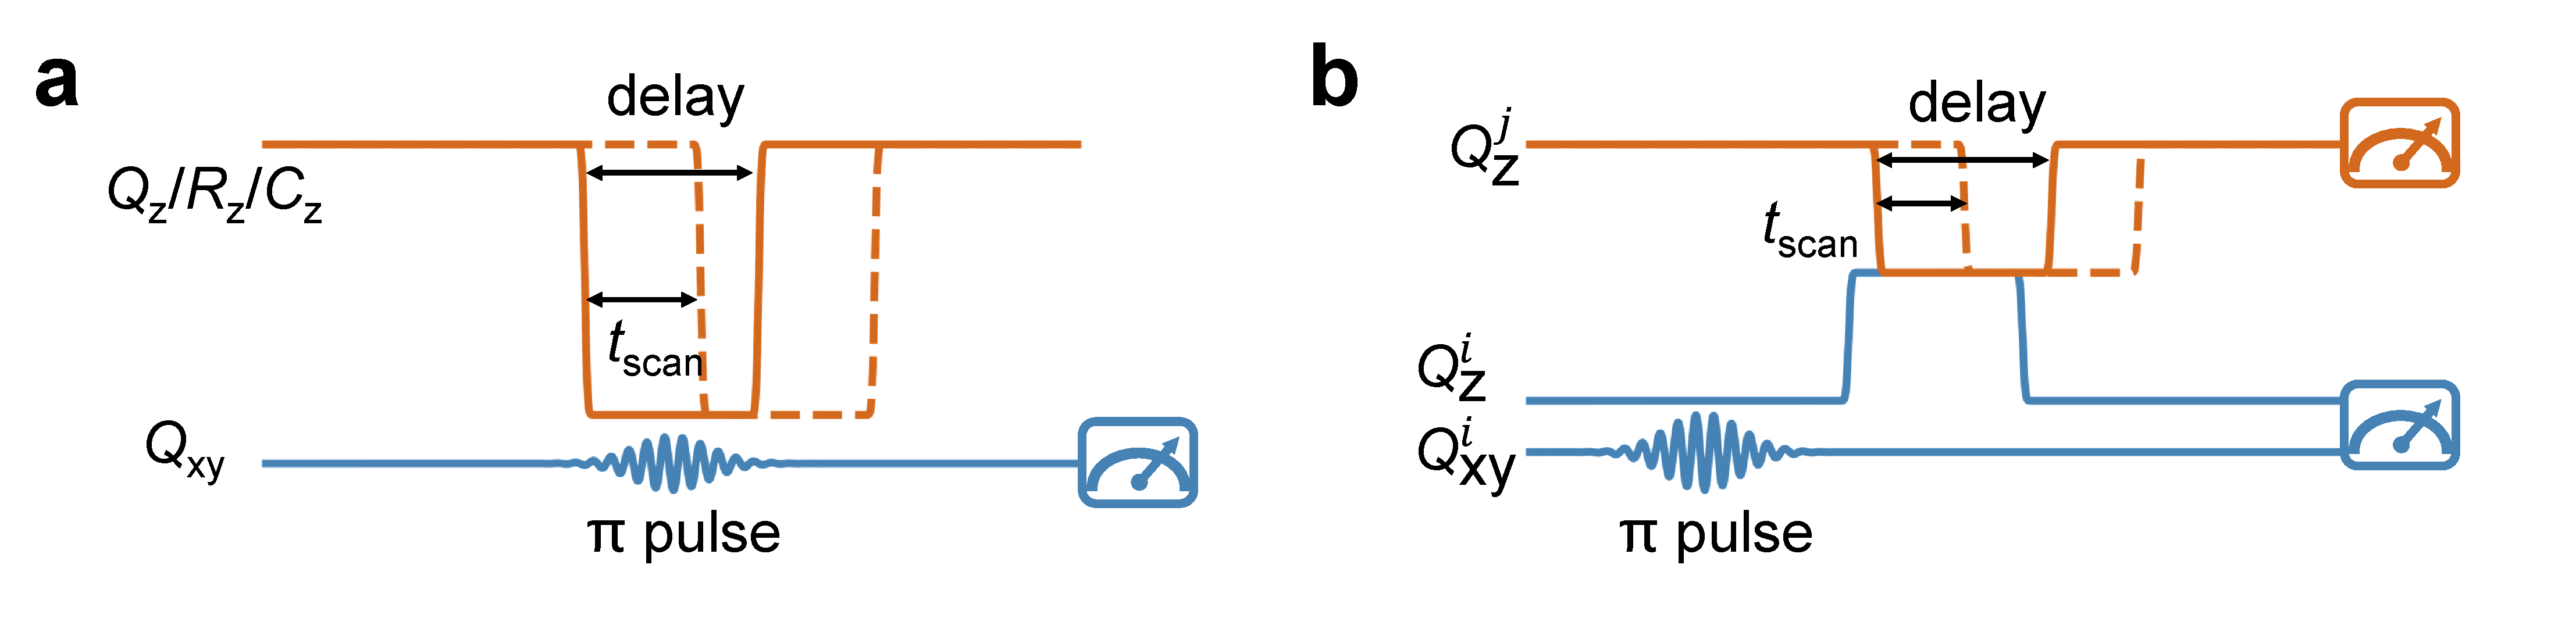
\includegraphics[width=1.0\linewidth]{suppFig/FigureSI_timing.pdf}
		\caption{\textbf{Timing alignment of qubits, couplers, and bus resonator.} \textbf{a}, Schematic of the experimental pulse sequence for synchronizing XY-pulses of qubits and the Z-pulses of qubits, couplers, or bus resonator, with the Z-pulse delay equal to the duration of a \(\pi\) pulse. \(Q_\text{xy}\) denotes the XY-channel of a qubit, while \(Q_\text{z}\), \(R_\text{z}\), and \(C_\text{z}\) denote the Z-channels of a qubit, the bus resonator, and a coupler, respectively. \textbf{b}, Schematic of the experimental pulse sequence for synchronizing Z-pulses of qubits, with the Z-pulse delay equal to one-quarter of the swap period between qubits. The notation \(Q^i_\text{xy}\) and \(Q^i_\text{z}\) represent the XY-channel and Z-channel of \(Q_1\), respectively. \(Q^j_\text{z}\) donates the Z-channel of \(Q_j\) with \(j = 2, \ldots, 14\). }
		\label{timing}
	\end{figure}
    
	\subsection{Pulse calibration}
	Precise control of Z-pulses is critical for realizing high-fidelity quantum state preparation and maintaining coherent evolution in superconducting quantum circuits. Because the frequencies of qubits and couplers are modulated by Z-pulses, thus any distortion in Z-pulses—particularly in the rising edge, falling edge, or flatness—can induce unintended frequency drifts. 
    
    To characterize distortions in qubit’s Z-pulse, we designed a pulse sequence to measure its tail, as shown in Supplementary Fig.~\ref{pulseshape}\textbf{a}. The measurement is performed in a region where the qubit’s frequency is highly sensitive to the Z-pulse amplitude, ensuring that even small distortions can also induce detectable frequency shifts. A long Z-pulse with a fixed amplitude is applied to the qubit’s Z-channel, generating a step-like signal. After a variable delay ($t_{\text{scan}}$), a $\pi$-pulse is applied to the qubit’s XY-channel at the idle frequency. Besides, a scanned Z-offset ($Z_{\text{scan}}$) is applied to the pulse sequence. The $\pi$-pulse excites the qubit to the |1⟩ state perfectly only when its frequency matches that of the $\pi$-pulse. The probability of the qubit being in the $|1\rangle$ state is measured as a function of the delay, as shown in Supplementary Fig.~\ref{pulseshape}\textbf{b}. The peak population of the $|1\rangle$ state for each delay provides time-resolved profile on the Z-pulse’s tail shape. 
    
    The calibration of Z-pulse distortions for couplers (or bus resonator) leverages their strong transverse coupling to nearby qubits, allowing the distortions of the coupler’s Z-line to be probed indirectly via the qubit’s excitation probability. The corresponding pulse sequence, shown in Supplementary Fig.~\ref{pulseshape}\textbf{d}, can capture the response of the coupler’s Z-pulse. Before characterizing Z-pulse distortions, the coupler is biased to an anti-crossing region with the adjacent qubit by applying a bias-pulse amplitude $Z_{\text{step}}$.
    In the Z-pulse distortions experiments, a single Z-pulse with amplitude ($Z_{\text{step}}$) is applied to the coupler, to generate a step-like signal. After a variable delay ($t_{\text{scan}}$), a time-varying $\pi$-pulse is applied to the adjacent qubit. The qubit is optimally excited to the $|1\rangle$ state when the qubit’s frequency matches the $\pi$-pulse frequency. The time-varying $\pi$-pulse ensures high temporal resolution for short-time distortions while preserving frequency resolution for long-time distortions. An additional Z-offset ($Z_{\text{scan}}$) is applied to the entire pulse sequence and scanned. When the offset compensates for the distortion, the qubit’s excitation probability is maximized, as shown in Supplementary Fig.~\ref{pulseshape}\textbf{e}. The detailed procedure of Z-pulse distortions is described in the ref.~\cite{PRA_ltm}.
    
    To correct these distortions, the measured data are fitted using a combination of polynomial and exponential functions, which effectively compensate for short-time and long-time distortions, respectively. The correction function is then incorporated into waveform generation to pre-compensate the Z-line signal. After correction, the full calibration sequence is repeated to verify convergence. Typically, two iterations are sufficient to achieve a near-ideal Z-pulse shape, as verified by the reduced distortion observed in Supplementary Fig. ~\ref{pulseshape}\textbf{c} and ~\ref{pulseshape}\textbf{f} compared to the significant distortion pre-correction.
    

	\begin{figure}
		\centering
		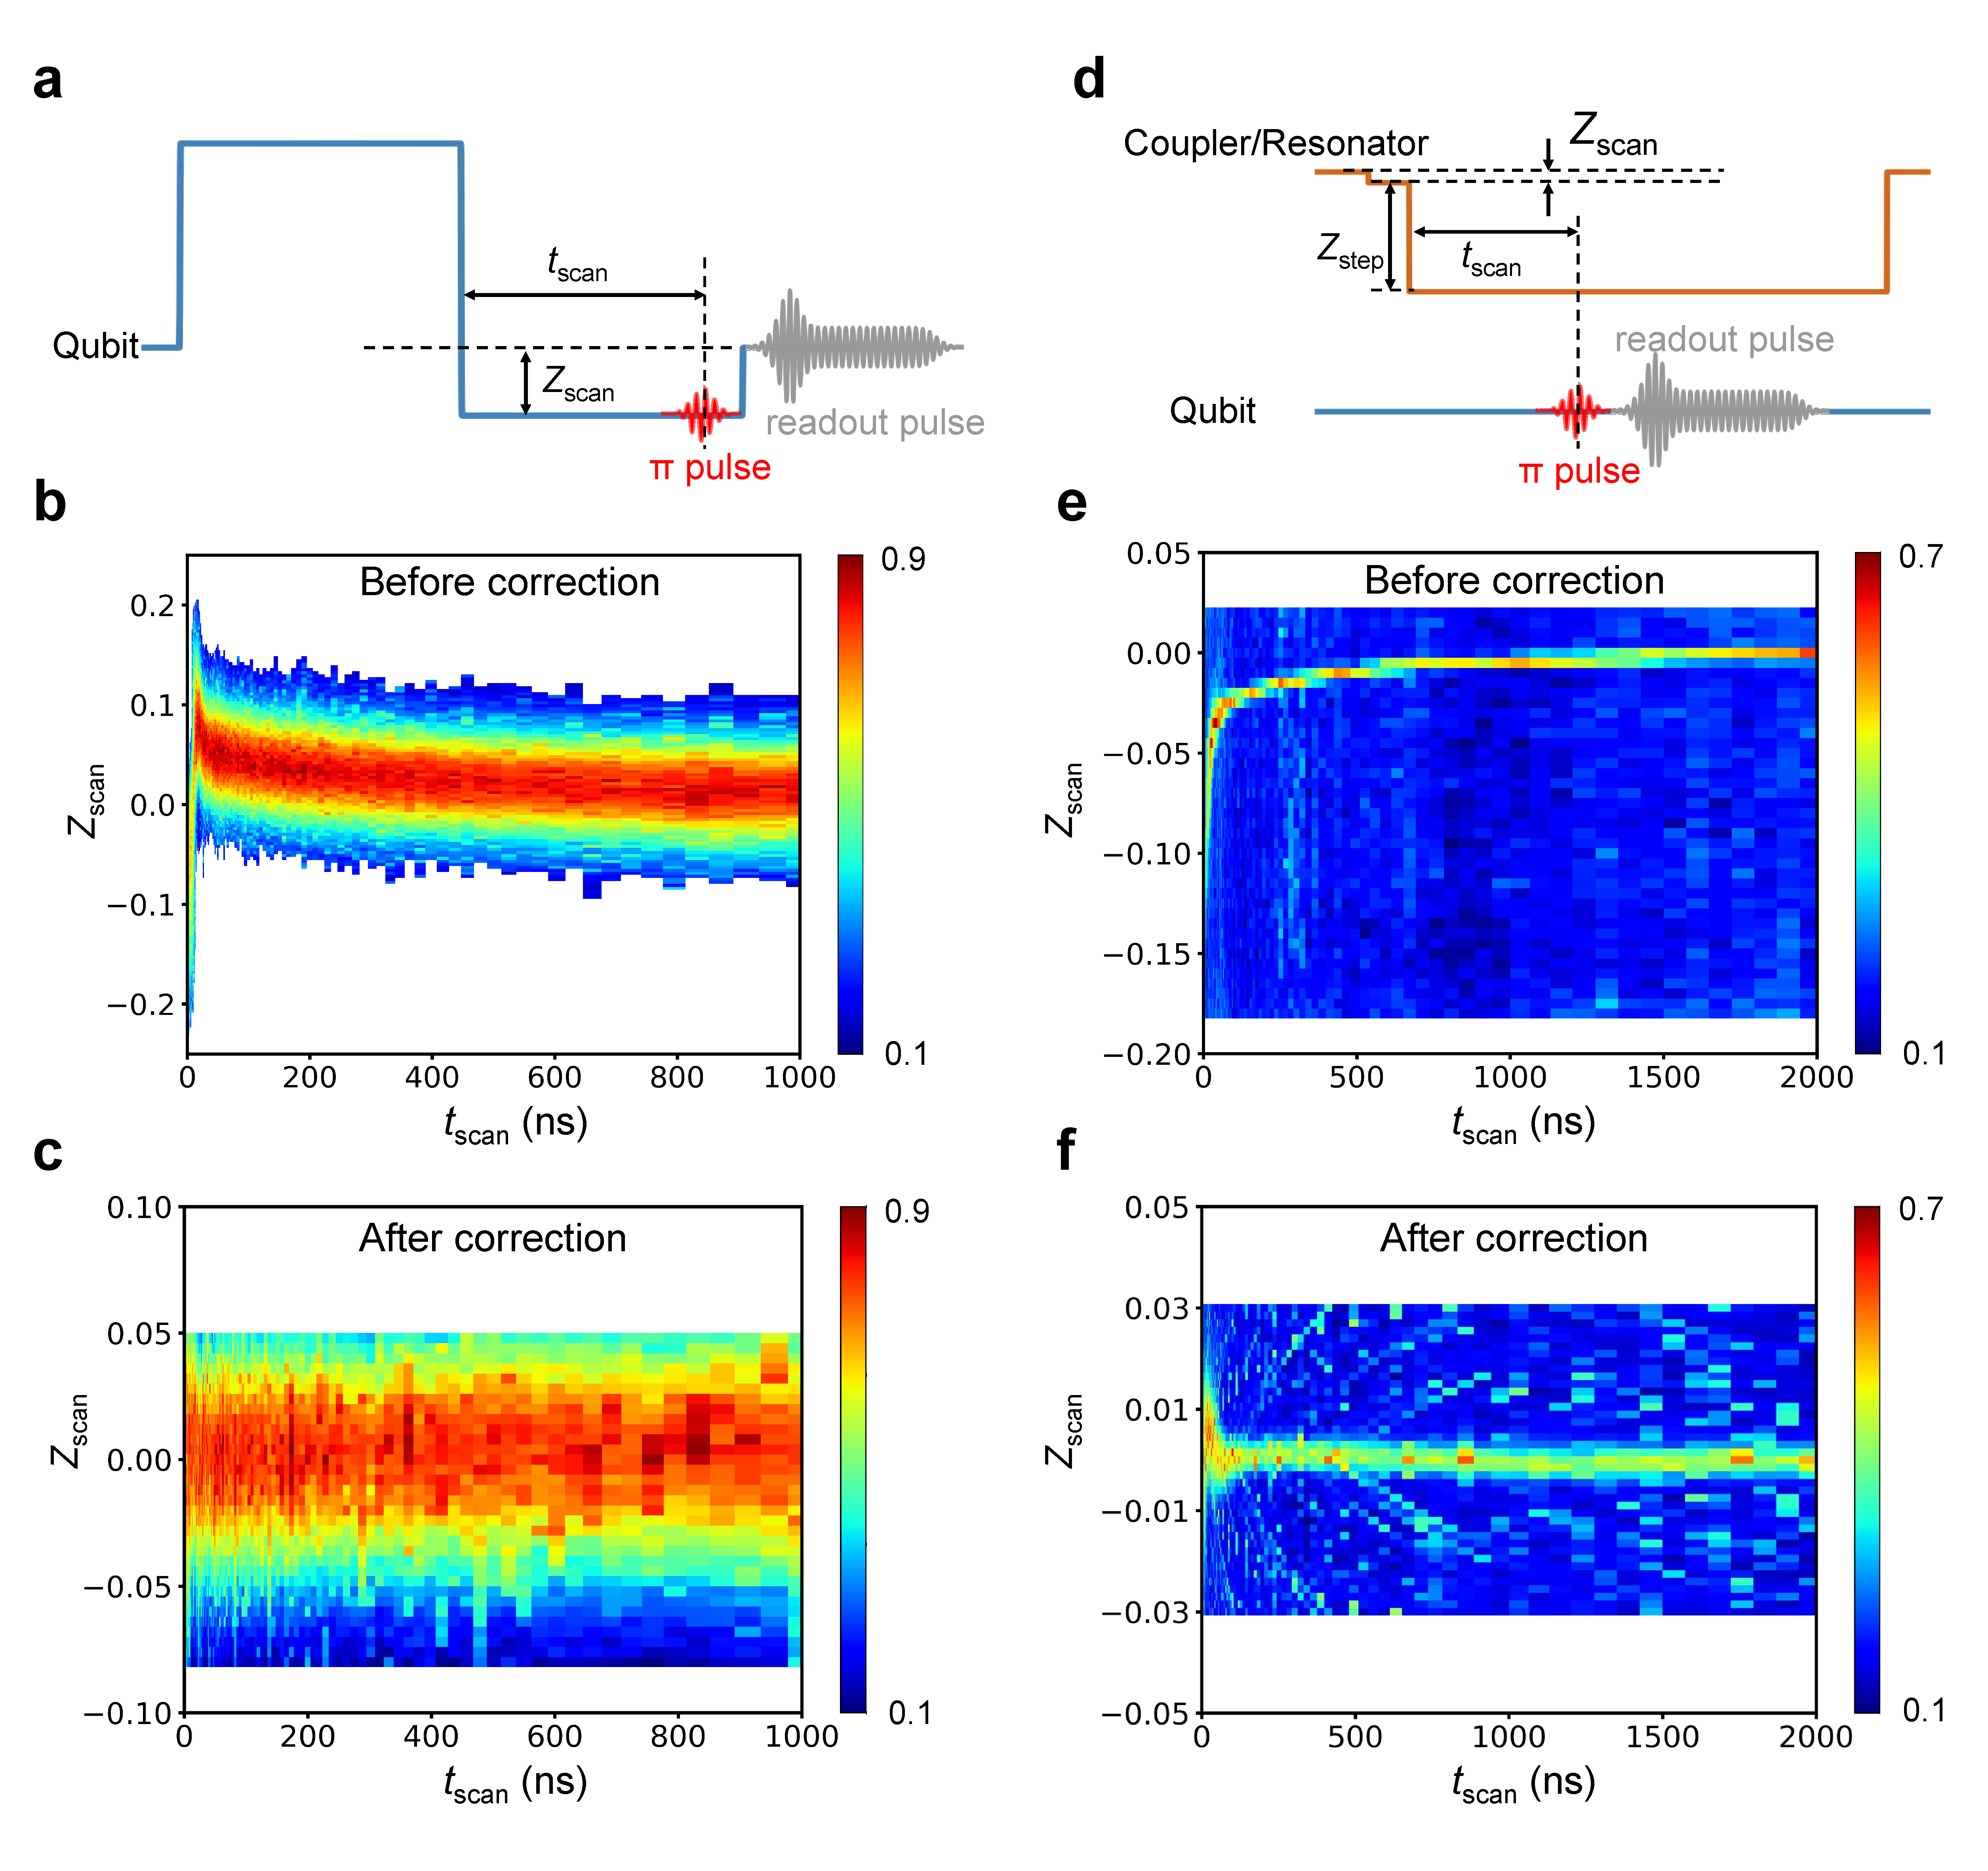
\includegraphics[width=1.0\linewidth]{suppFig/FigureSI_pulseshape.pdf}
		\caption{\textbf{Calibration of the Z pulse distortion for qubits and couplers.} \textbf{a}, Schematic of the experimental pulse sequence for correcting Z-pulse distortion of qubits.
		\textbf{b} and \textbf{c}, Probability of the $\ket{1}$ state for qubits before and after correction, respectively.
		\textbf{d}, Schematic of the experimental pulse sequence for correcting Z-pulse distortion of couplers. \textbf{e} and \textbf{f}, Probability of the $\ket{1}$ state for couplers before and after correction, respectively.}
		\label{pulseshape}
	\end{figure}
	
    \clearpage
    \newpage


	\section{Modulation of coupling strength}
	
	\subsection{Quantization of a tunable resonator circuit}

We consider a system in which two qubits are coupled to a shared bus resonator. The equivalent circuit is depicted in Supplementary Fig.~\ref{equivalent circuit}. The effective capacitance and inductance of the resonator for each qubit depend on their respective coupling positions. We denote these as $C_r^j$ and $L_r^j$ for \textit{j}=1, 2. The circuit parameters satisfy the condition $C_{j},C_r^j\gg C_{jr}\gg C_{12}$, where $C_{jr}$ is the coupling capacitance between qubit \textit{j} and the resonator, and $C_{12}$ is the direct capacitance between the two qubits.

\begin{figure}[h]
    \centering
    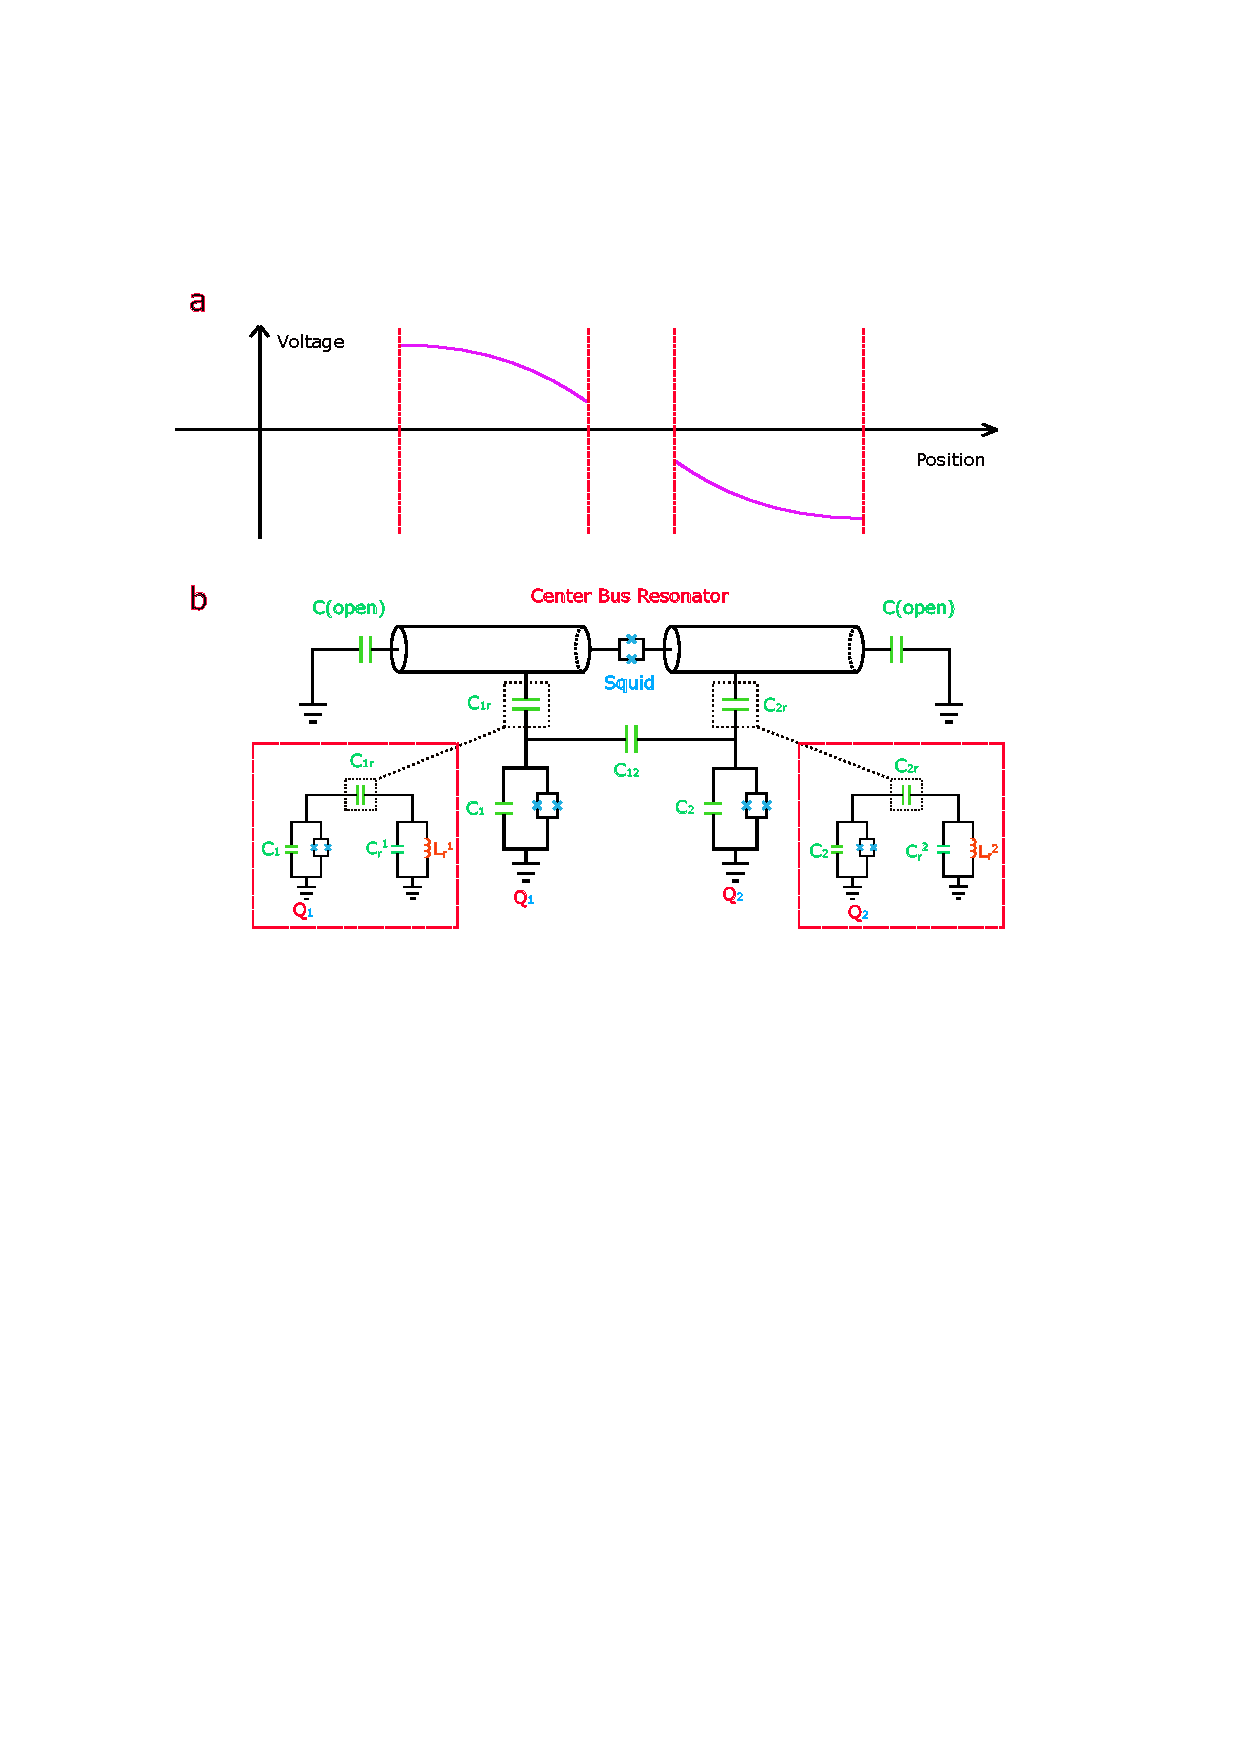
\includegraphics[width=0.85\textwidth]{suppFig/equivalent_circuit.pdf}
    \caption{\textbf{Equivalent circuit model for two qubits coupled to a frquency-tunable central bus resonator.} \textbf{a}, Voltage distribution of the central bus resonator. \textbf{b}, Equivalent circuit model of the central bus resonator coupled to two qubits, where the resonator exhibits distinct effective capacitance and inductance for each qubit, relative to their coupling positions.}
    \label{equivalent circuit}
\end{figure}

For a half-wavelength resonant cavity, the voltage at different coupling positions is determined by the spatial variation of the electromagnetic field. We use \( \dot{\varphi}_r^j \) represents resonator’s voltage at the coupling position for qubit \( j \). And their ratio is
\begin{equation}
    \frac{\dot{\varphi _r^1}}{\dot{\varphi _r^2}} = \frac{\cos (\beta x_1)}{\cos (\beta x_2)} = \frac{1}{k},
\end{equation}
where \( \beta = \omega / v \), \( v \) is the electromagnetic wave propagation speed in the waveguide, and \( x_j \) is the distance from the coupling position of qubit \( j \) to the open end of the resonator. The parameter \( k \), reflecting the relative phase of the field, can be positive or negative. The effective capacitance at each coupling position is
\begin{equation}
    C_r^j=\frac{C_rl}{2\left(\cos \beta x_j\right)^2 },
\end{equation}
here \( C_rl \) is a constant related to the resonator’s geometry. Consequently, we have 
\begin{equation}
\frac{1}{2} C_r^1 \dot{\varphi_r^1}^2 = \frac{1}{2} C_r^2 \dot{\varphi_r^2}^2,
\end{equation}
indicating equivalence in the kinetic and potential energy contributions regardless of whether \( \varphi_r^1 \) or \( \varphi_r^2 \) is used.
The system Lagrangian is composed of kinetic (\( T \)) and potential (\( U \)) energy terms, expressed using node fluxes \( \varphi_1 \), \( \varphi_2 \), and \( \varphi_r^j \). The kinetic energy is
\begin{equation}
\begin{aligned}
    T &=\frac{1}{2}\left[C_1 \dot{\varphi_1}^2 + C_2 \dot{\varphi_2}^2 + C_r^1 \dot{\varphi_r^1}^2 \right] \\
    &+ \frac{1}{2} \left[C_{1r}\left(\dot{\varphi_1}- \dot{\varphi_r^1}\right)^2 +C_{2r}\left(\dot{\varphi_2}- \dot{\varphi_r^2}\right)^2 +C_{12}\left(\dot{\varphi_1}- \dot{\varphi_2}\right)^2 \right].
\end{aligned}
\end{equation}
Using \( \dot{\varphi_r^2} = k \dot{\varphi_r^1} \) and \( |k| = \sqrt{C_r^1 / C_r^2} \), we eliminate \( \dot{\varphi_r^2} \), yielding
\begin{equation}
\begin{aligned}
T &= \frac{1}{2} \left[ C_1 \dot{\varphi_1}^2 + C_2 \dot{\varphi_2}^2 + C_r^1 \dot{\varphi_r^1}^2 \right] + \frac{1}{2} \left[ C_{1r} \left( \dot{\varphi_1} - \dot{\varphi_r^1} \right)^2 + C_{2r} \left( \dot{\varphi_2} - k \dot{\varphi_r^1} \right)^2 + C_{12} \left( \dot{\varphi_1} - \dot{\varphi_2} \right)^2 \right].
\end{aligned}
\end{equation}
The kinetic energy can be expressed in compact form as \( T = \frac{1}{2} \dot{\vec{\varphi}}^\top C \dot{\vec{\varphi}} \), where \( \vec{\varphi} = [\varphi_1, \varphi_2, \varphi_r^1]^\top \) and \( C \) is the 3 × 3 capacitance matrix
\begin{equation}
\begin{aligned}
C=\begin{bmatrix}
C_1+C_{12}+C_{1r} &  -C_{12} & -C_{1r} \\
-C_{12} &  C_2+C_{12}+C_{2r} & -k C_{2r} \\
-C_{1r} &  -k C_{2r} & C_r^1+C_{1r}+k^2 C_{2r} \\
\end{bmatrix}.
\end{aligned}
\end{equation}
The inverse capacitance matrix, approximated under the condition \( C_j, C_r^j \gg C_{jr} \gg C_{12} \), 
\begin{equation}
\begin{aligned}
C^{-1} \approx \begin{bmatrix}
\frac{1}{C_1} &  \frac{ k C_{1r} C_{2r}  + C_r^1 C_{12}}{C_{1} C_{2} C_{r^1}} & \frac{C_{1r}}{C_1 C_r^1}\\
\frac{k C_{1r} C_{2r}  + C_r^1  C_{12}}{C_{1} C_{2} C_{r^1}}  & \frac{1}{C_2} & k \frac{C_{2r}}{C_2 C_r^1}\\
\frac{C_{1r}}{C_1 C_r^1} & k \frac{C_{2r}}{C_2 C_r^1} & \frac{1}{C_r^1} \\
\end{bmatrix}.
\end{aligned}
\end{equation}
The conjugate charge vector is \( \vec{q} = C \dot{\vec{\varphi}} \), and the classical Hamiltonian is
\begin{equation}
H = \frac{1}{2} \vec{q}^\top C^{-1} \vec{q} + U. 
\end{equation}
Here,the potential energy $U$ includes the Josephson energies of the qubits and the inductive energy of the resonator
 \begin{equation}
    \begin{aligned}
        U &= E_{J_1}\left[1-\cos\left(\frac{2\pi}{\Phi_0}\varphi_1\right)\right]+E_{J_2}\left[1-\cos\left(\frac{2\pi}{\Phi_0}\varphi_2\right)\right]+\frac{{\varphi_r^1}^2}{2L_r^1},
    \end{aligned}
\end{equation}
where \( E_{J_j} \) is the Josephson energy of qubit \( j \), and \( \Phi_0 = h / (2e) \) is the flux quantum. Quantizing the system, we promote \( \vec{q} \) and \( \vec{\varphi} \) to operators satisfying \( [\hat{\varphi}_\lambda, \hat{q}_{\lambda'}] = i \hbar \delta_{\lambda \lambda'} \). The quantized Hamiltonian is
\begin{equation}
\begin{aligned}
    \hat{H} = & 4E_{c_1}\left(\hat{n_1}\right)^2-E_{J_1}\cos\left(\frac{2\pi}{\Phi_0}\hat{\varphi_1}\right)
    +4E_{c_2}\left(\hat{n_2}\right)^2-E_{J_2}\cos\left(\frac{2\pi}{\Phi_0}\hat{\varphi_2}\right)    +4E_{c_r^1}\left(\hat{n_r^1}\right)^2+\frac{{\hat{\varphi_r^1}}^2}{2L_r^1}\\
    &+8\frac{C_{1r}}{\sqrt{C_1 C_r^1}}\sqrt{E_{c_1}E_{c_r^1}}\left(\hat{n_1}\hat{n_r^1}\right)+8\frac{k C_{2r}}{\sqrt{C_2 C_r^1}}\sqrt{E_{c_2}E_{c_r^1}}\left(\hat{n_2}\hat{n_r^1}\right)\\
    &+8\left(\frac{ k C_{1r} C_{2r} + C_r^1  C_{12}}{ C_{r^1} \sqrt{C_{1} C_{2} }}\right)\sqrt{E_{c_1}E_{c_2}}\left(\hat{n_1}\hat{n_2}\right),\\
\end{aligned}
\end{equation}
where \( \hat{n}_\lambda = \hat{q}_\lambda / (2e) \) is the Cooper-pair number operator, and \( E_{c_\lambda} = e^2 / (2 C_\lambda) \) is the charging energy for \( \lambda = 1, 2, r \).

In the transmon regime (\( E_{J_\lambda} / E_{c_\lambda} \gg 1 \)), the qubits and resonator behave as weakly anharmonic oscillators. We approximate the system as coupled Duffing oscillators (\( \hbar = 1 \)):
\begin{equation}
\hat{H} = \hat{H}_1 + \hat{H}_2 + \hat{H}_r + \hat{H}_{1r} + \hat{H}_{2r} + \hat{H}_{12}, 
\end{equation}
where the individual mode Hamiltonians are
\begin{equation}
 \hat{H}_\lambda = \omega_\lambda \hat{b}_\lambda^\dagger \hat{b}_\lambda + \frac{\alpha_\lambda}{2} \hat{b}_\lambda^\dagger \hat{b}_\lambda^\dagger \hat{b}_\lambda \hat{b}_\lambda, \quad \lambda = 1, 2, r, 
 \end{equation}
with anharmonicities
\begin{equation}
 \alpha_\lambda = -E_{c_\lambda}, \quad \lambda = 1, 2. 
\end{equation}
The interaction terms are
\begin{equation}
 \hat{H}_{jr} = g_{jr} \left( \hat{b}_j^\dagger \hat{b}_r + \hat{b}_j \hat{b}_r^\dagger - \hat{b}_j^\dagger \hat{b}_r^\dagger - \hat{b}_j \hat{b}_r \right), \quad j = 1, 2, 
\end{equation}
\begin{equation}
 \hat{H}_{12} = g_{12} \left( \hat{b}_1^\dagger \hat{b}_2 + \hat{b}_1 \hat{b}_2^\dagger - \hat{b}_1^\dagger \hat{b}_2^\dagger - \hat{b}_1 \hat{b}_2 \right), 
\end{equation}
with coupling strengths
\begin{equation}
 g_{1r} = \frac{1}{2} \frac{C_{1r}}{\sqrt{C_1 C_r^1}} \sqrt{\omega_1 \omega_r}, 
\end{equation}
\begin{equation}
 g_{2r} = \frac{1}{2} \frac{k C_{2r}}{\sqrt{C_2 C_r^1}} \sqrt{\omega_2 \omega_r} = \frac{1}{2} \frac{k}{|k|} \frac{C_{2r}}{\sqrt{C_2 C_r^2}} \sqrt{\omega_2 \omega_r},
\end{equation}
\begin{equation}
 g_{12} = \frac{1}{2} \frac{k C_{1r} C_{2r} + C_{12} C_r^1}{\sqrt{C_1 C_2} C_r^1} \sqrt{\omega_1 \omega_2} = \frac{1}{2} (1 + \eta) \frac{C_{12}}{\sqrt{C_1 C_2}} \sqrt{\omega_1 \omega_2},
\end{equation}
where
\begin{equation}
\eta = \frac{k}{|k|} \frac{C_{1r} C_{2r}}{C_{12} \sqrt{C_r^1 C_r^2}}. 
\end{equation}
The sign of \( k \), determined by the relative positions of the qubits along the resonator (\( \cos \beta x_j \)), influences the sign of \( g_{2r} \). This sign is crucial for accurately modeling the system’s dynamics, particularly in experiments requiring precise control coupling strength between qubits. 

To eliminate the qubit-resonator interactions and obtain an effective qubit-qubit coupling, we apply the Schrieffer-Wolff transformation:
\begin{equation}
\hat{U} = \exp \left\{ \sum_{j=1,2} \left[ \frac{g_{jr}}{\Delta_{jr}} \left( \hat{b}_j^\dagger \hat{b}_r - \hat{b}_j \hat{b}_r^\dagger \right) - \frac{g_{jr}}{\Sigma_{jr}} \left( \hat{b}_j^\dagger \hat{b}_r^\dagger - \hat{b}_j \hat{b}_r \right) \right] \right\},
\end{equation}
where
\begin{equation}
\Delta_{jr} = \omega_j - \omega_r, \quad \Sigma_{jr} = \omega_j + \omega_r. 
\end{equation}
The transformed Hamiltonian is
\begin{equation}
\hat{\widetilde{H}} = \hat{U} \hat{H} \hat{U}^\dagger = \widetilde{\omega_1} \hat{b}_1^\dagger \hat{b}_1 + \frac{\widetilde{\alpha_1}}{2} \hat{b}_1^\dagger \hat{b}_1^\dagger \hat{b}_1 \hat{b}_1 + \widetilde{\omega_2} \hat{b}_2^\dagger \hat{b}_2 + \frac{\widetilde{\alpha_2}}{2} \hat{b}_2^\dagger \hat{b}_2^\dagger \hat{b}_2 \hat{b}_2 + \widetilde{g}_{12} \left( \hat{b}_1^\dagger \hat{b}_2 + \hat{b}_1 \hat{b}_2^\dagger \right),
\end{equation}
with
\begin{equation}
\widetilde{\omega_1} \approx \omega_1 + g_{1r}^2 \left( \frac{1}{\Delta_{1r}} - \frac{1}{\Sigma_{1r}} \right), \widetilde{\alpha_1} \approx \alpha_1,
\end{equation}
\begin{equation}
\widetilde{\omega_2} \approx \omega_2 + g_{2r}^2 \left( \frac{1}{\Delta_{2r}} - \frac{1}{\Sigma_{2r}} \right),  \widetilde{\alpha_2} \approx \alpha_2,
\end{equation}
\begin{equation}
\widetilde{g}_{12} = \frac{g_{1r} g_{2r}}{2} \left( \frac{1}{\Delta_{1r}} + \frac{1}{\Delta_{2r}} - \frac{1}{\Sigma_{1r}} - \frac{1}{\Sigma_{2r}} \right) + g_{12}.
\end{equation}

For nearest-neighbor qubits, the presence of a tunable coupler introduces additional frequency shifts and modifies the effective qubit-qubit coupling. Take the coupler into consideration, the effective frequencies are
\begin{equation} \widetilde{\omega_1} = \omega_1 + g_{1r}^2 \left( \frac{1}{\Delta_{1r}} - \frac{1}{\Sigma_{1r}} \right) + g_{1c}^2 \left( \frac{1}{\Delta_{1c}} - \frac{1}{\Sigma_{1c}} \right), \end{equation}
\begin{equation} \widetilde{\omega_2} = \omega_2 + g_{2r}^2 \left( \frac{1}{\Delta_{2r}} - \frac{1}{\Sigma_{2r}} \right) + g_{2c}^2 \left( \frac{1}{\Delta_{2c}} - \frac{1}{\Sigma_{2c}} \right), \end{equation}
where \( g_{jc} \), \( \Delta_{jc} \), and \( \Sigma_{jc} \) are the coupling strength, detuning, and sum frequency between the qubit and coupler, respectively. The effective qubit-qubit coupling becomes
\begin{equation} 
\widetilde{g}_{12} = \frac{g_{1r} g_{2r}}{2} \left( \frac{1}{\Delta_{1r}} + \frac{1}{\Delta_{2r}} - \frac{1}{\Sigma_{1r}} - \frac{1}{\Sigma_{2r}} \right) + \frac{g_{1c} g_{2c}}{2} \left( \frac{1}{\Delta_{1c}} + \frac{1}{\Delta_{2c}} - \frac{1}{\Sigma_{1c}} - \frac{1}{\Sigma_{2c}} \right) + g_{12}, 
\end{equation}
where
\begin{equation} g_{12} = \frac{1}{2} \frac{k C_{1r} C_{2r} C_c + C_{1c} C_{2c} C_r^1 + C_{12} C_r^1 C_c}{\sqrt{C_1 C_2} C_r^1 C_c} \sqrt{\omega_1 \omega_2}. \end{equation}

The above analysis actually neglects the coupling between the coupler and the bus resonator, a simplification justified by the negligible interaction strength ($g_{rc} \ll g_{qr}, g_{qc}$ and \( C_{rc} \ll C_{qr}, C_{qc}\)). This allows the coupler-resonator interaction to be safely ignored in our model, simplifying the analysis without significant loss of accuracy. Crucially, our analysis reveals that in our experimental system, the effective coupling strength between neighboring qubits arises from three primary contributions: (1) coupling mediated by the bus resonator, (2) coupling mediated by the coupler, and (3) direct coupling $g_{12}$ induced by the capacitive structure. Notably, while the effective coupling form mediated by the resonator is analogous to that of the coupler, the resonator-mediated interaction may involve opposite signs for the coupling strengths \( g_{1r} \) and \( g_{2r} \), resulting in distinct coupling effects compared to the coupler.

	\subsection{Experimental control of coupling strength}

Supplementary Figure~\ref{geff_bus_coupler} presents the experimentally measured variation in coupling strength between pairs of qubits, modulated by the bus resonator tuned above the qubit frequencies (i.e., \( \Delta_{qr} < 0 \)). As the frequency of bus resonator decreases, the coupling strength between qubits \( Q_{11} \) and \( Q_{12} \) gradually reduces, similar to the effect observed with the coupler~\cite{yan_coupler_2018}. However, for qubits \( Q_{13} \) and \( Q_{14} \), the coupling strength increases as the bus resonator frequency decreases, in contrast to the behavior observed for \( Q_{11} \) and \( Q_{12} \). This difference in behavior arises from the relative signs of the qubit–resonator coupling strengths: \( g_{11r} \) and \( g_{12r} \) have the same sign, whereas \( g_{13r} \) and \( g_{14r} \) have opposite signs. In fact, qubits located on the same side of the central resonator exhibit coupling strengths similar to that observed between \( Q_{11} \) and \( Q_{12} \). By contrast, qubits positioned on opposite sides of the central resonator display coupling characteristics analogous to those of \( Q_{13} \) and \( Q_{14} \), reflecting sign differences in their respective qubit–resonator couplings.

As the frequency of the central resonator decreases further—while remaining higher than the qubit frequencies—the coupling strength between $Q_{11}$ and $Q_{12}$ diminishes toward zero and then transitions to negative values. In contrast, the coupling strength between $Q_{13}$ and $Q_{14}$ exhibits a sustained increase, retaining a positive magnitude. Intriguingly, the effective sign of the coupling strength between qubits can be reversed by applying an additional $\pi$ phase. To ensure consistent initial phase alignment across all qubits, we adopt the approach detailed in ref.~\cite{10_Qubit_2017}. 
Subsequently, an additional $\pi$ phase is applied to the qubits on one side of the central resonator, rendering the coupling strengths between all qubits negative.
In the intermediate coupling regime ($r \approx 1$), the long-range coupling is tuned to around $-2$ MHz, with nearest-neighbor coupling strengths adjusted to $-2$ MHz through the modulation of couplers. A comprehensive coupling matrix for this configuration is provided in Supplementary Figure~\ref{r1}.
To reach the strong short-range coupling regime (\(r \approx10\)), the central resonator is tuned to its maximum frequency, resulting in an average long-range coupling strength of approximately \(0.5\)~MHz. Nearest-neighbor coupling strengths are then set to $-5$ MHz via the couplers, as depicted in Supplementary Figure~\ref{r10}.


	\begin{figure}
		\centering
		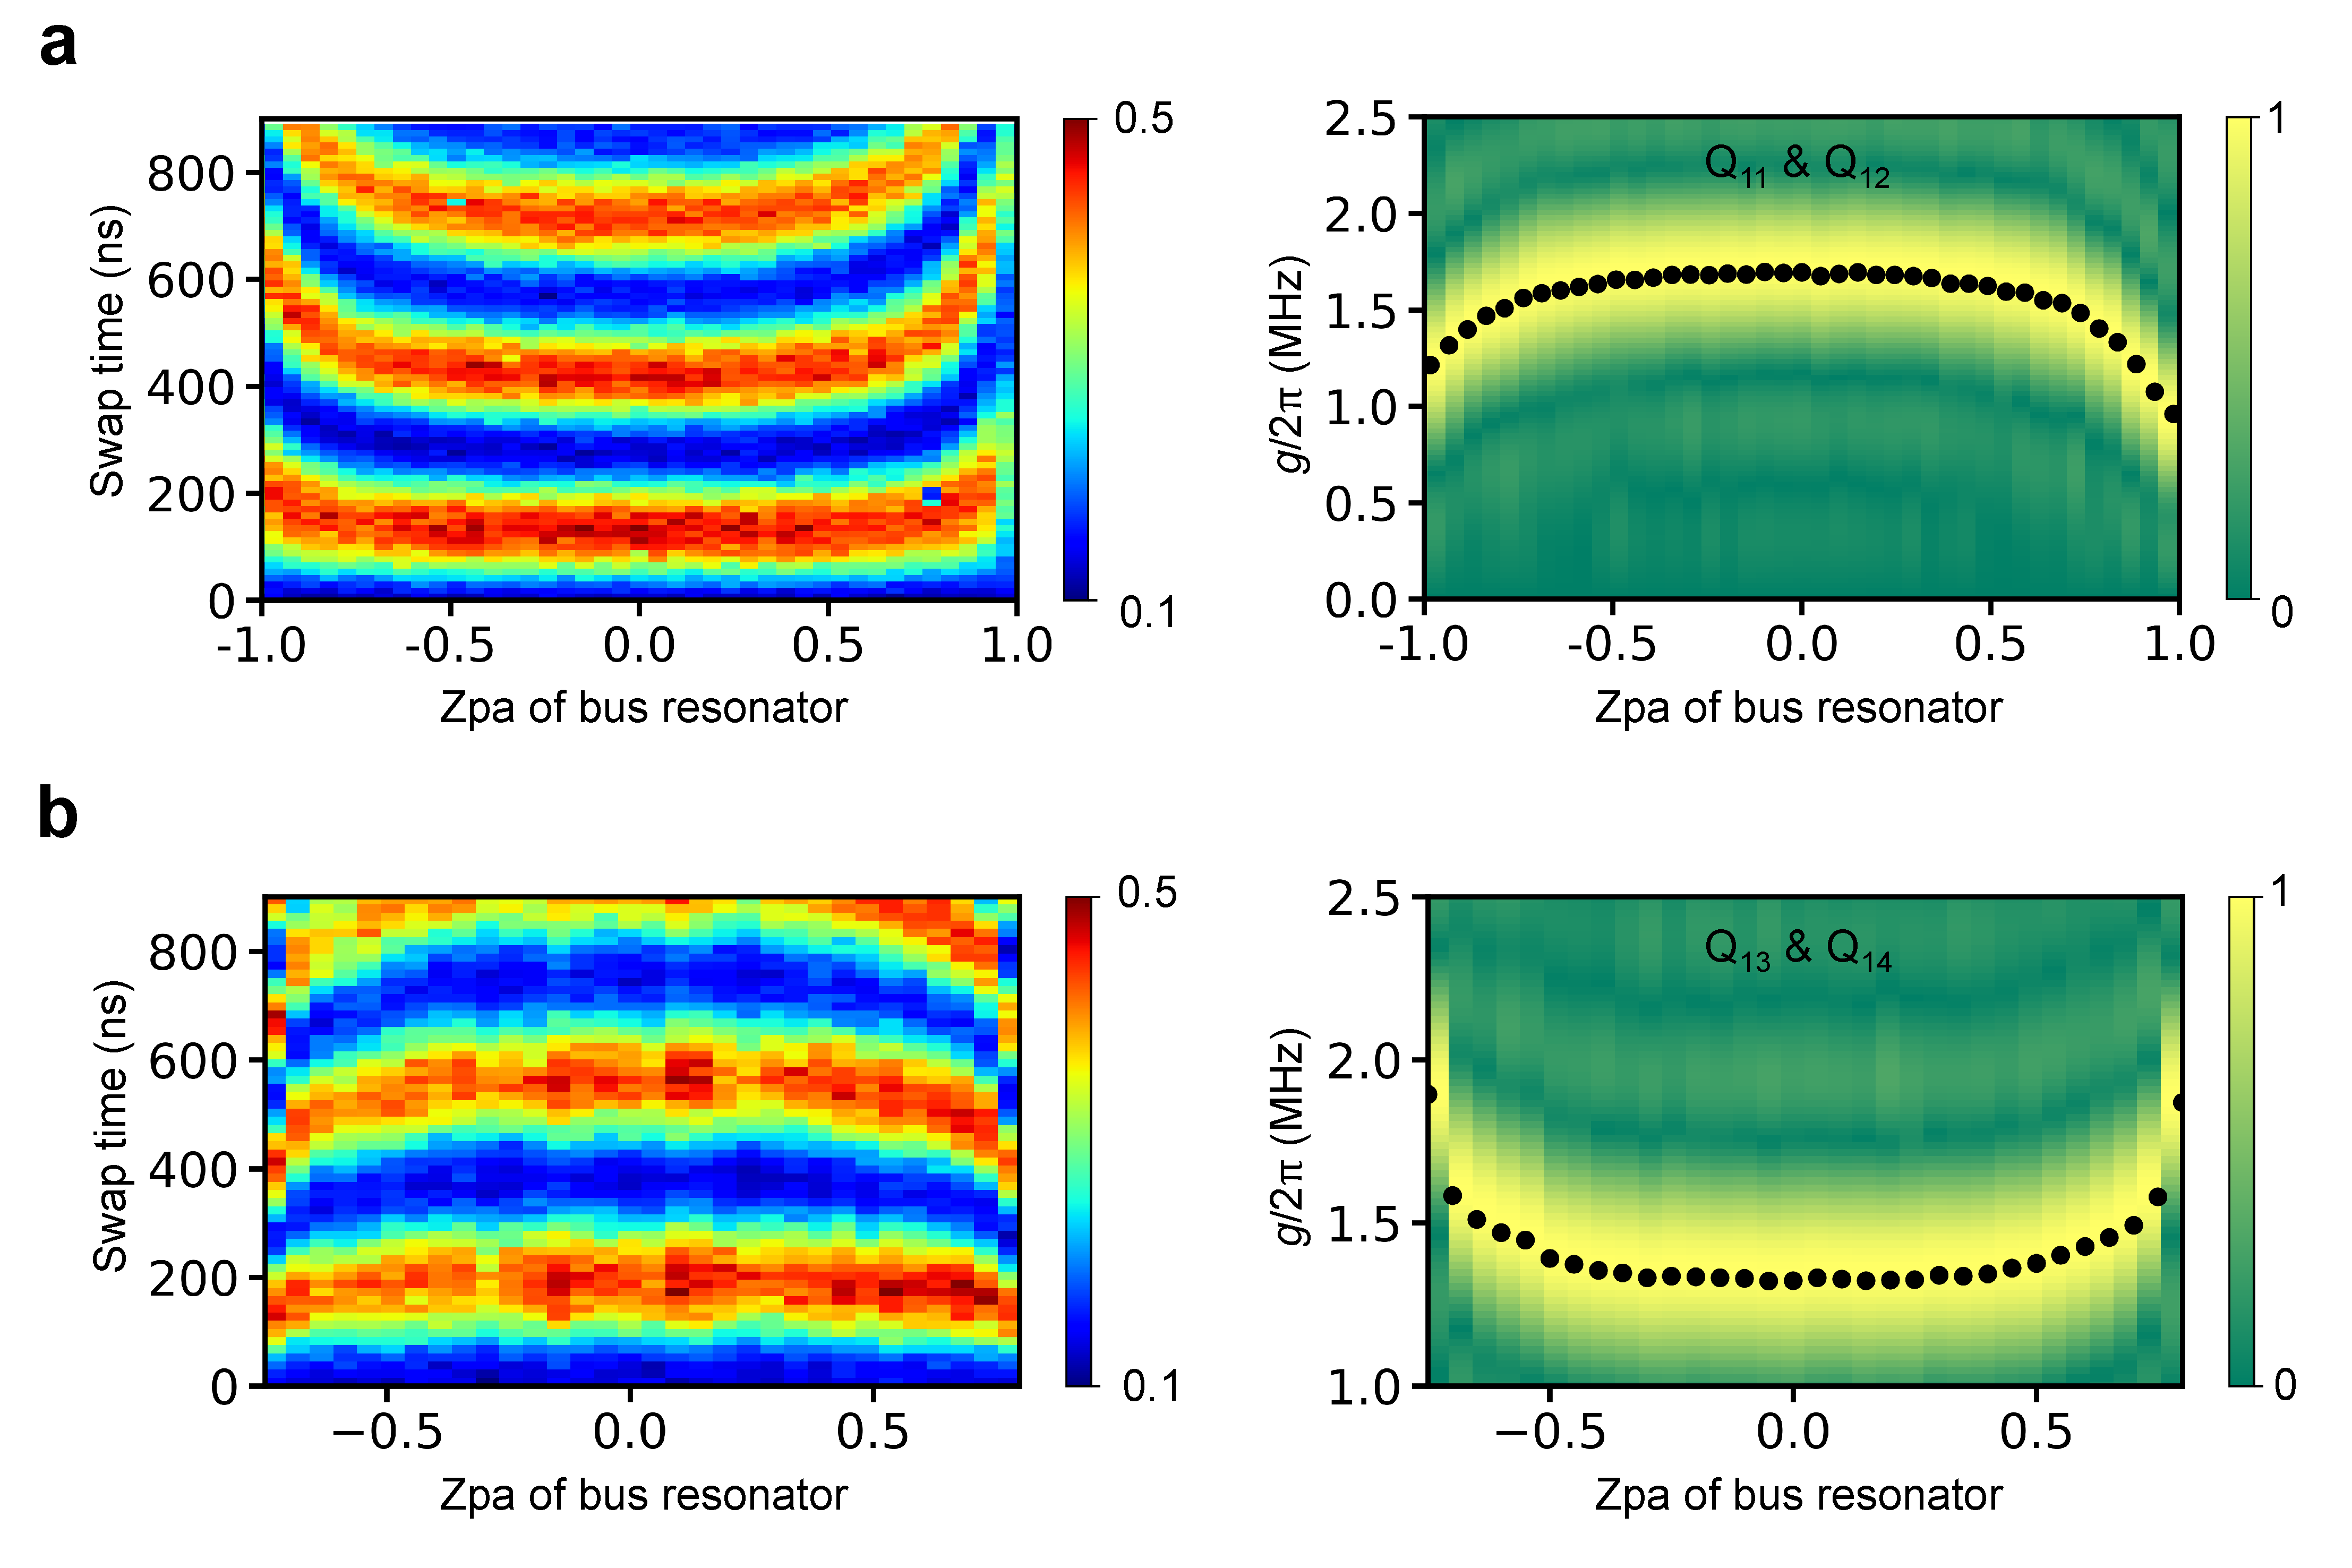
\includegraphics[width=1.0\linewidth]{suppFig/FigureSI_geff_bus_coupler.pdf}
		\caption{\textbf{Modulation of qubit–qubit coupling \(g/2\pi\) by the central bus resonator.} The coupling strength between \( Q_{11} \) and \( Q_{12} \) (\textbf{a}) , and between \( Q_{13} \) and \( Q_{14} \) (\textbf{b}), are measured as a function of the bus resonator’s Z-pulse amplitude (Zpa) through two-qubit swap spectroscopy. Left panels display experimental swap spectroscopy data, while the right panels show the corresponding coupling strengths \(g/2\pi\).}
		\label{geff_bus_coupler}
	\end{figure}

	\begin{figure}
		\centering
		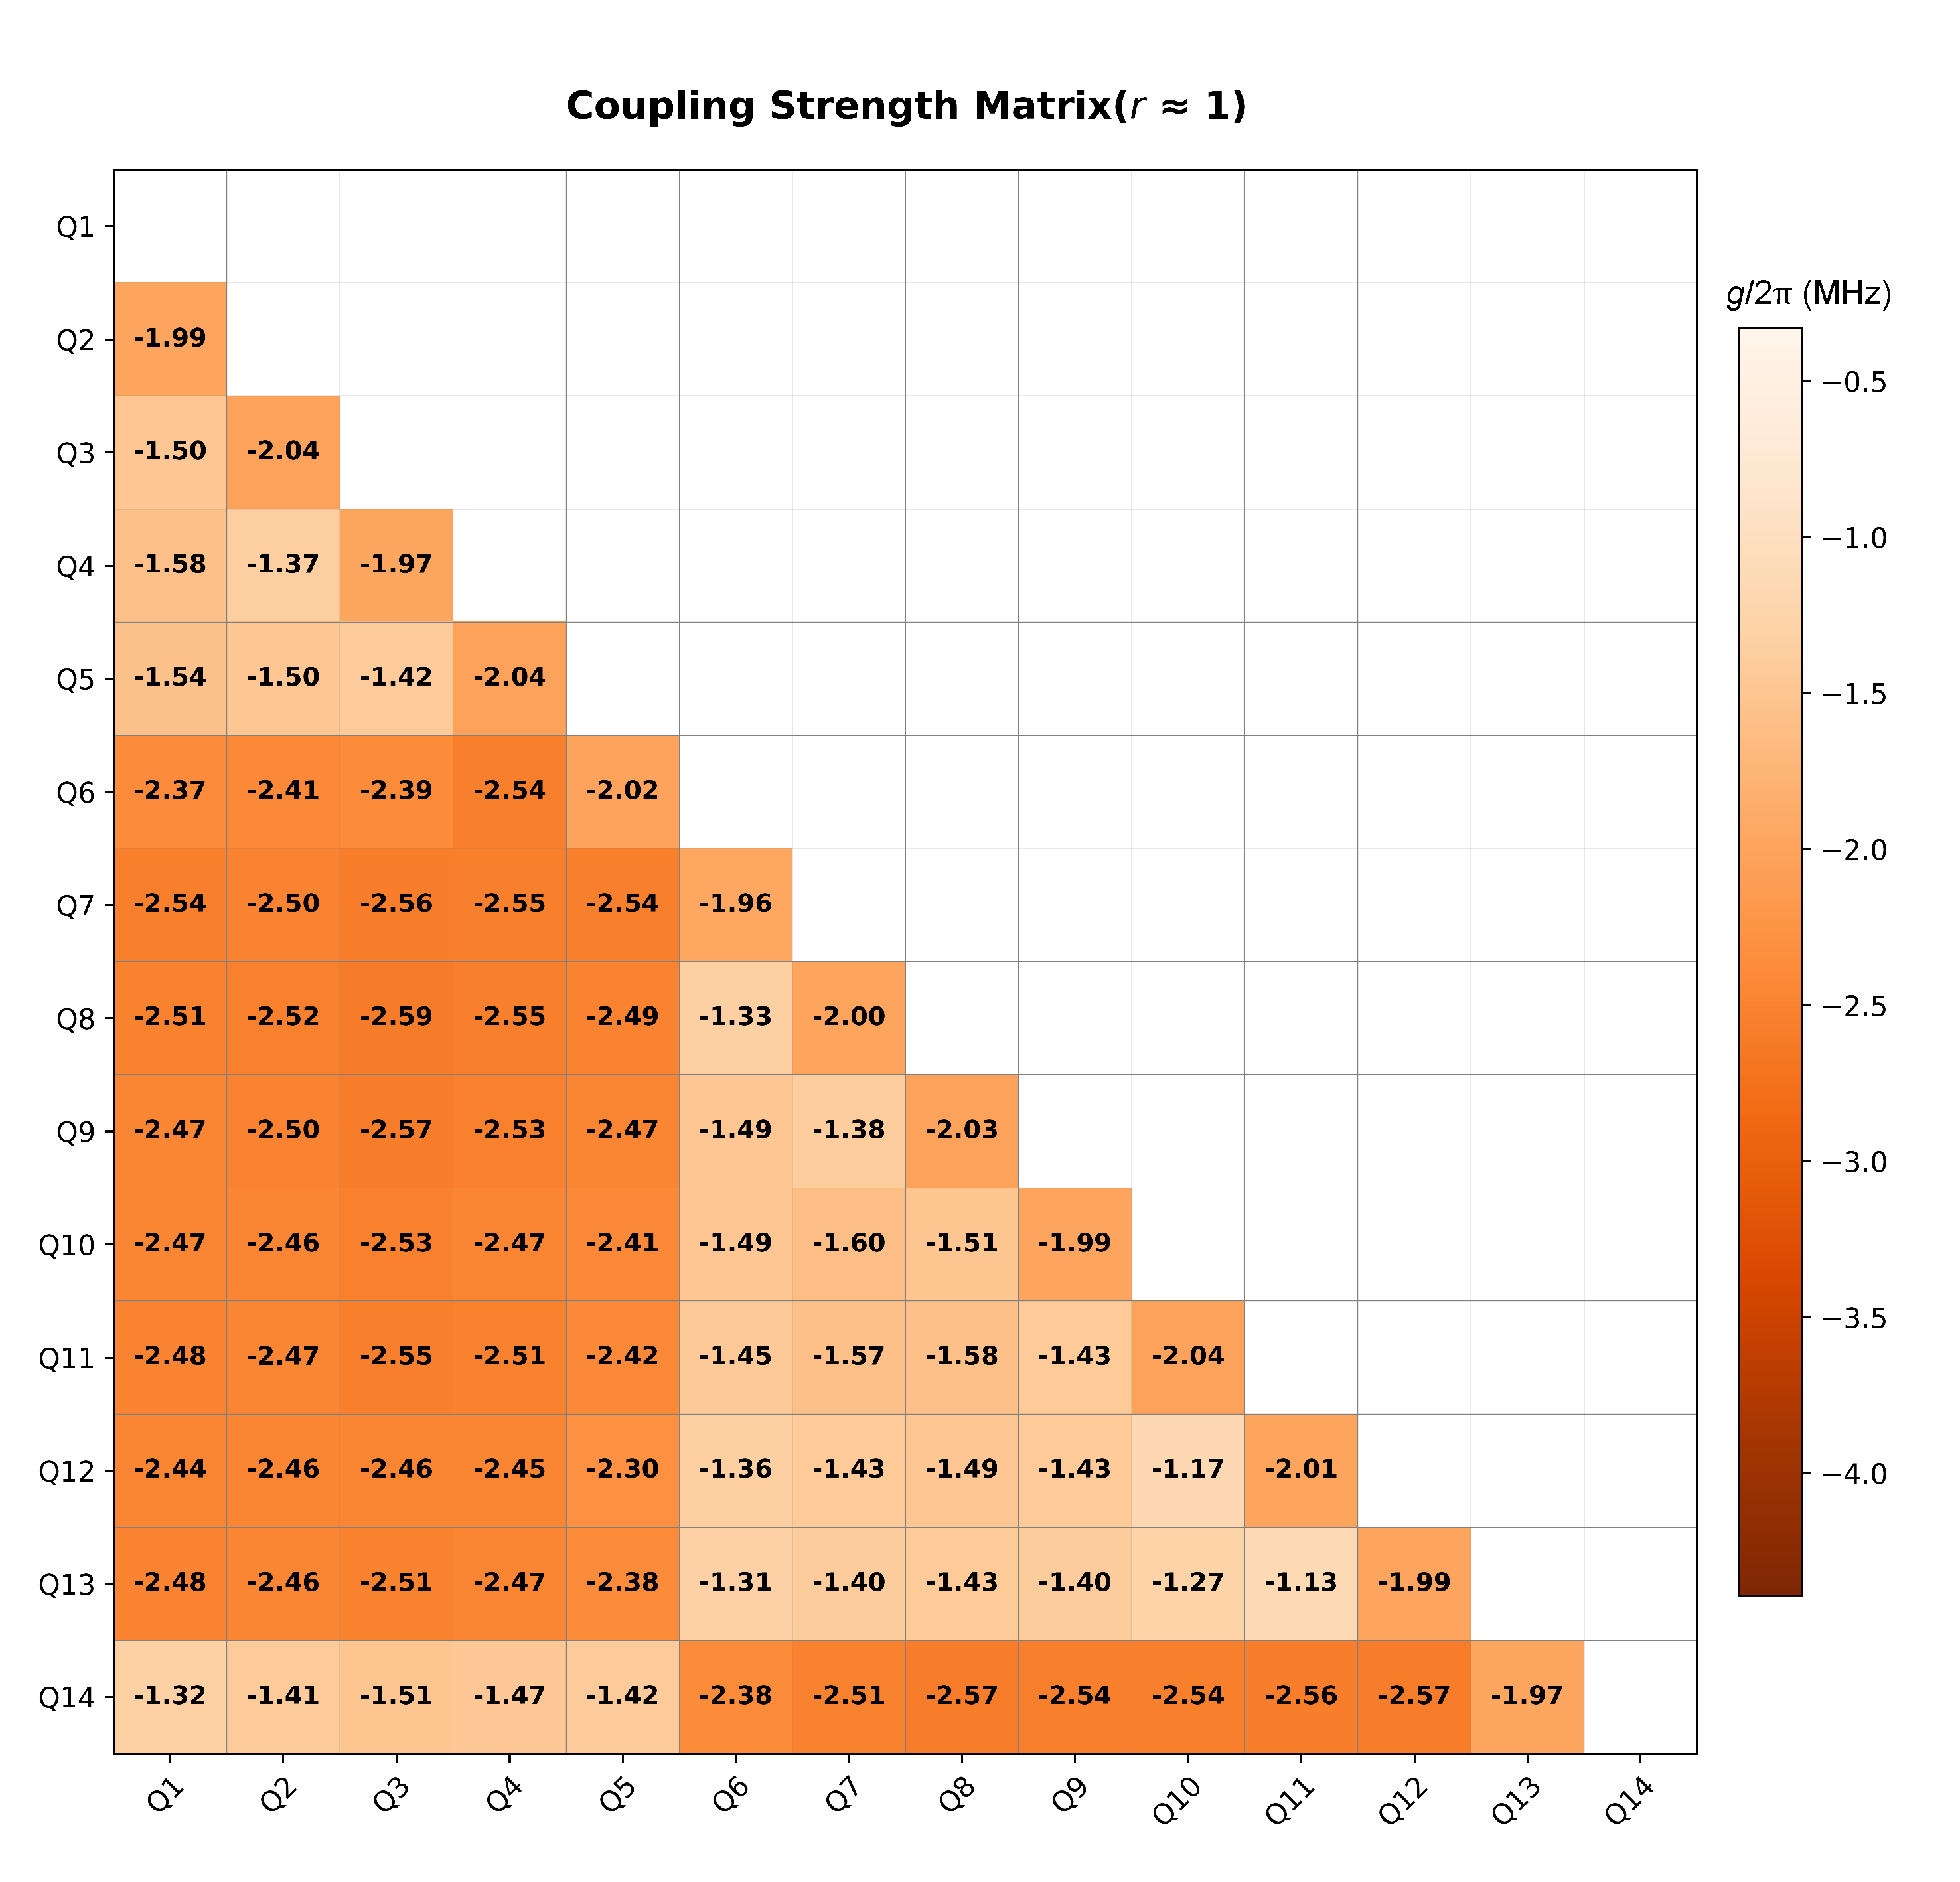
\includegraphics[width=1.0\linewidth]{suppFig/FigureSI_g_r1.pdf}
		\caption{\textbf{Coupling strength matrix in the intermediate coupling regime ($r\approx1$).} }
		\label{r1}
	\end{figure}

	\begin{figure}
		\centering
		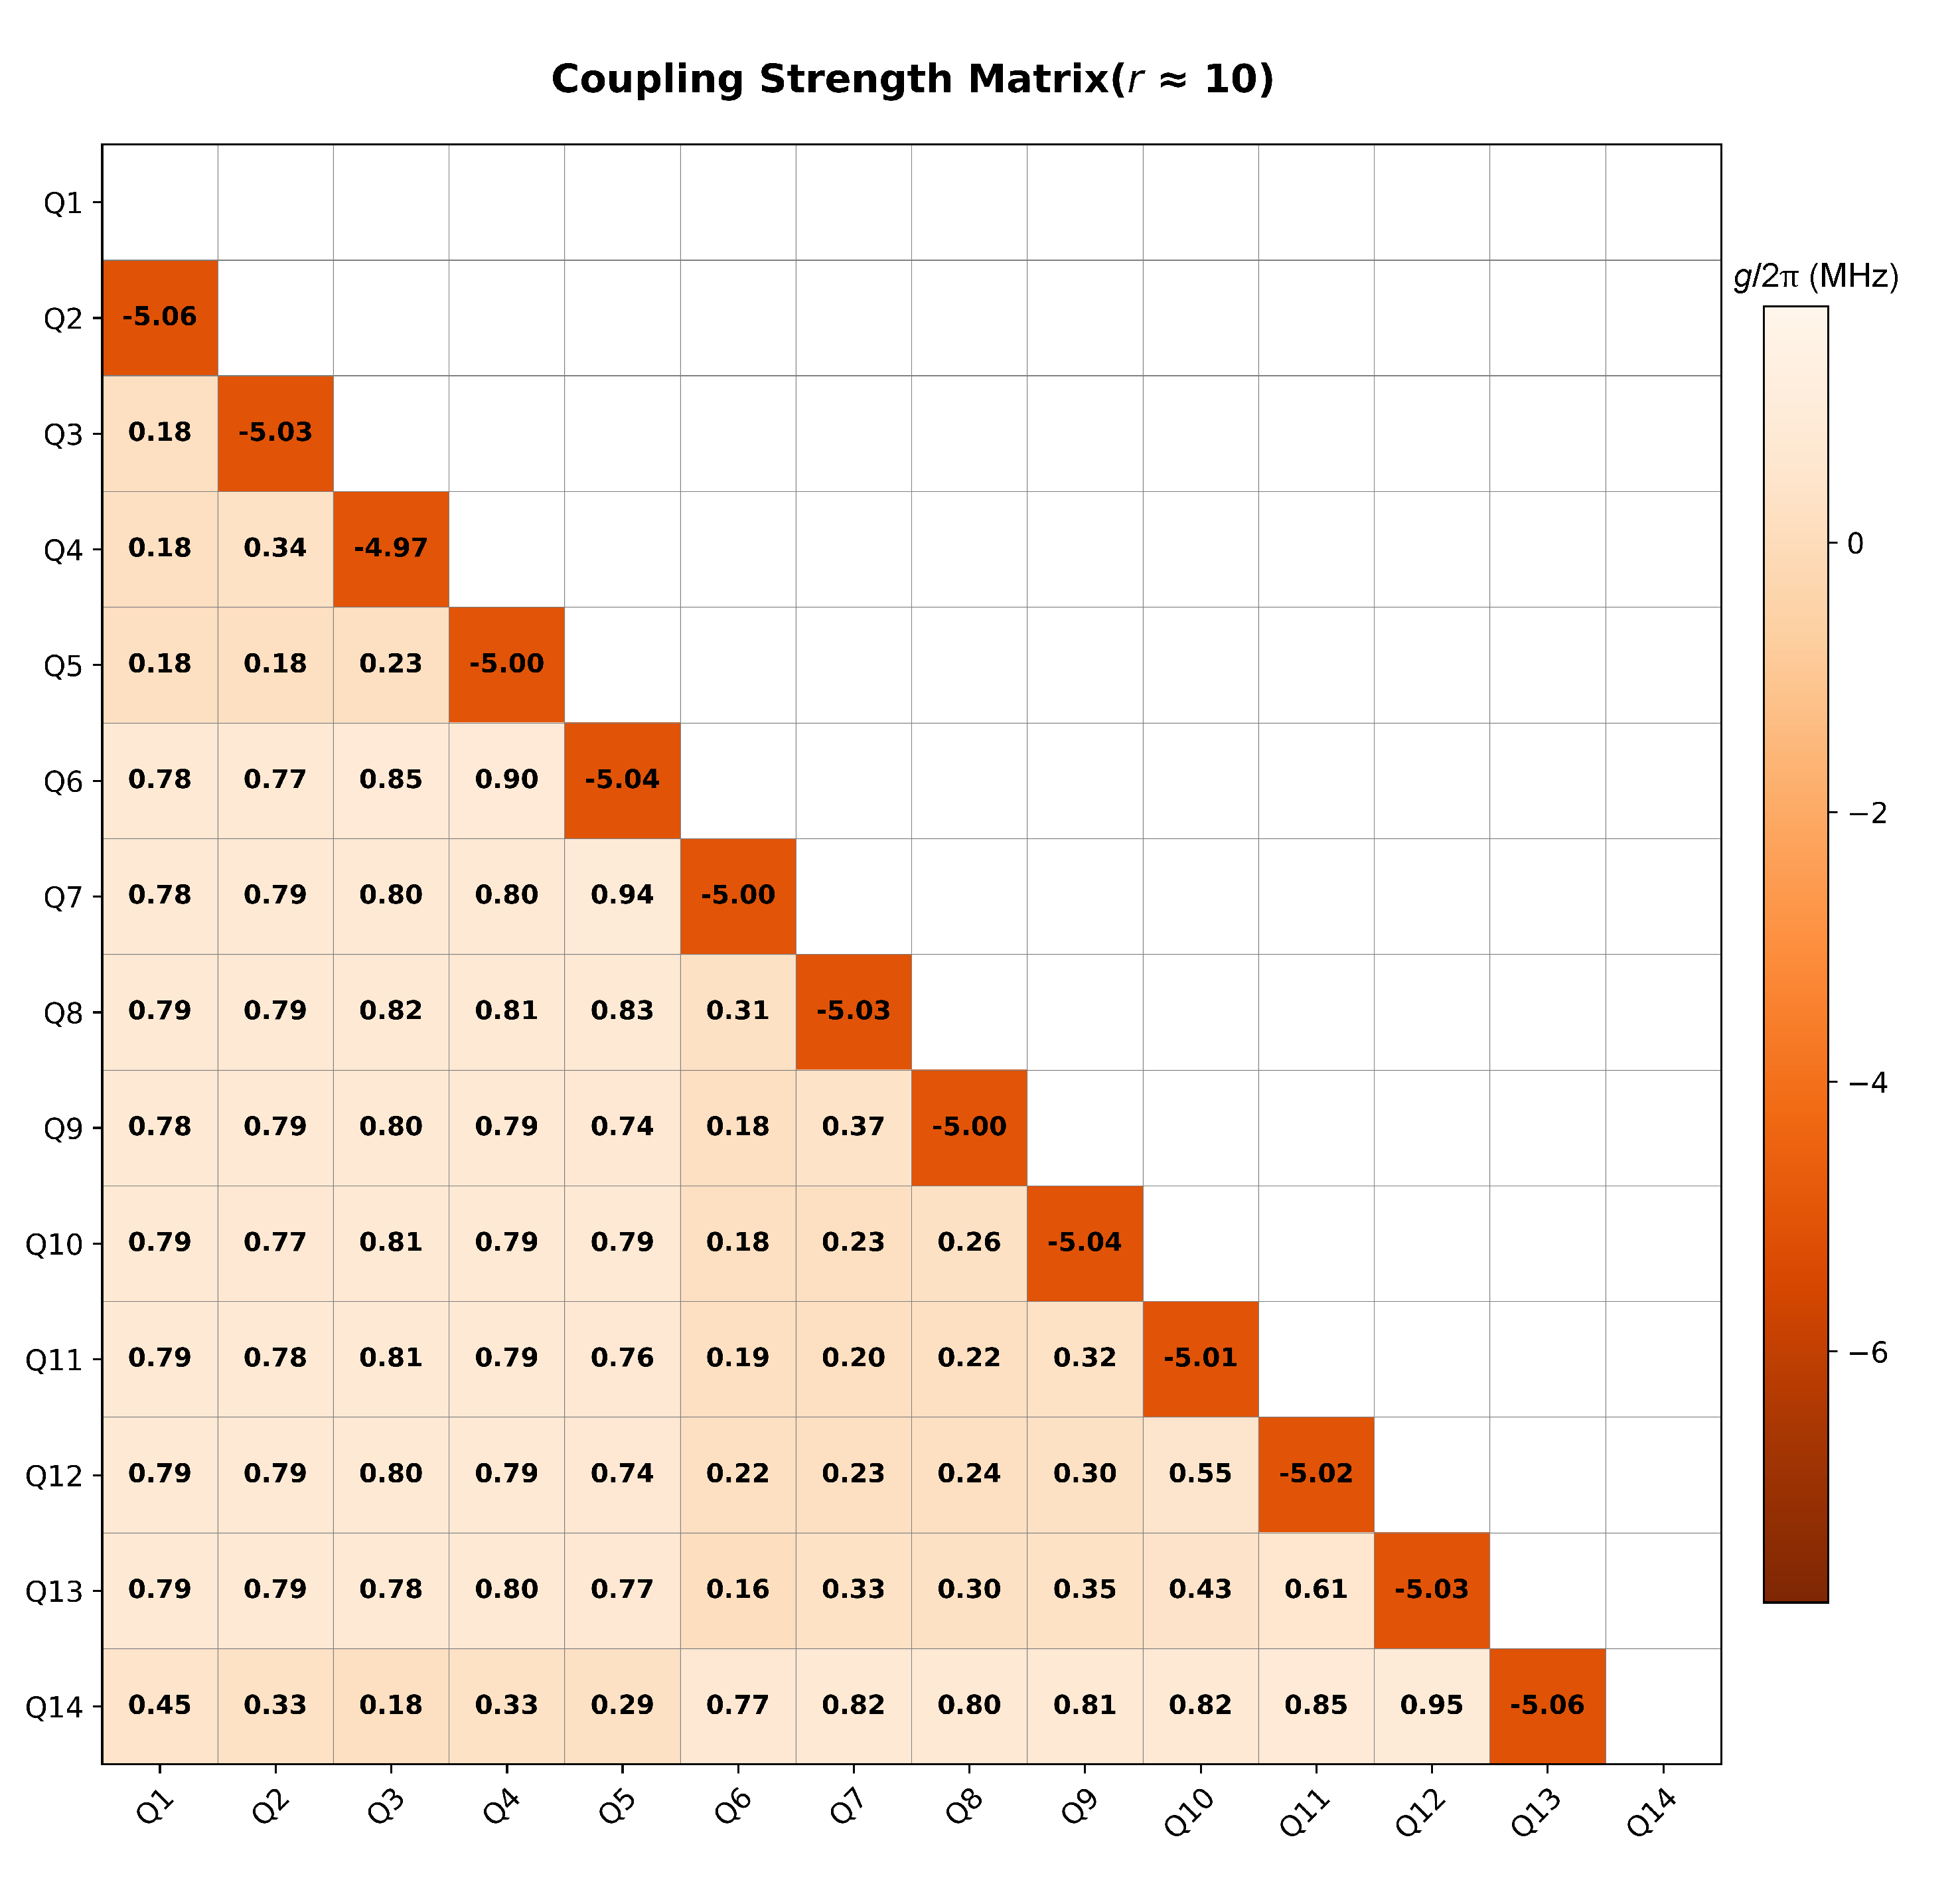
\includegraphics[width=1.0\linewidth]{suppFig/FigureSI_g_r10.pdf}
		\caption{\textbf{Coupling strength matrix in the strong short-range coupling regime ($r\approx10$).} }
		\label{r10}
	\end{figure}
	
	\clearpage
	\newpage
	
    \section{Numerical simulation}
     
    \subsection{EA dynamics in strong short-range interaction regime}
     
    We consider an ideal model of superconducting circuits described by Eq.~\eqref{hamiltonian}, with system size $N=14$ and open boundary conditions. The Hamiltonian is given by:
    \begin{equation}
    H = \sum_{i=1}^{N-1} \left( \sigma_x^i\sigma_x^{i+1} + \sigma_y^i\sigma_y^{i+1} \right) + g \sum_{i+1<j} \left( \sigma_x^i\sigma_x^{j} + \sigma_y^i\sigma_y^{j} \right),
    \end{equation}
    where nearest-neighbor interactions are uniform across all sites, long-range interactions exhibit analogous homogeneity and $g=1/r$ represents the strength of long range interaction. 
    Supplementary Fig.~\ref{fig:tunable.r} displays the EA dynamics for the terminal subsystem $[Q_1,Q_2,Q_3]$ at $g=0, 0.1, 0.15, 0.2,$ and $0.25$. The QME is observed for $g<0.15$ but disappears for $g>0.15$. 
    
    \begin{figure}[t]
    \centering
    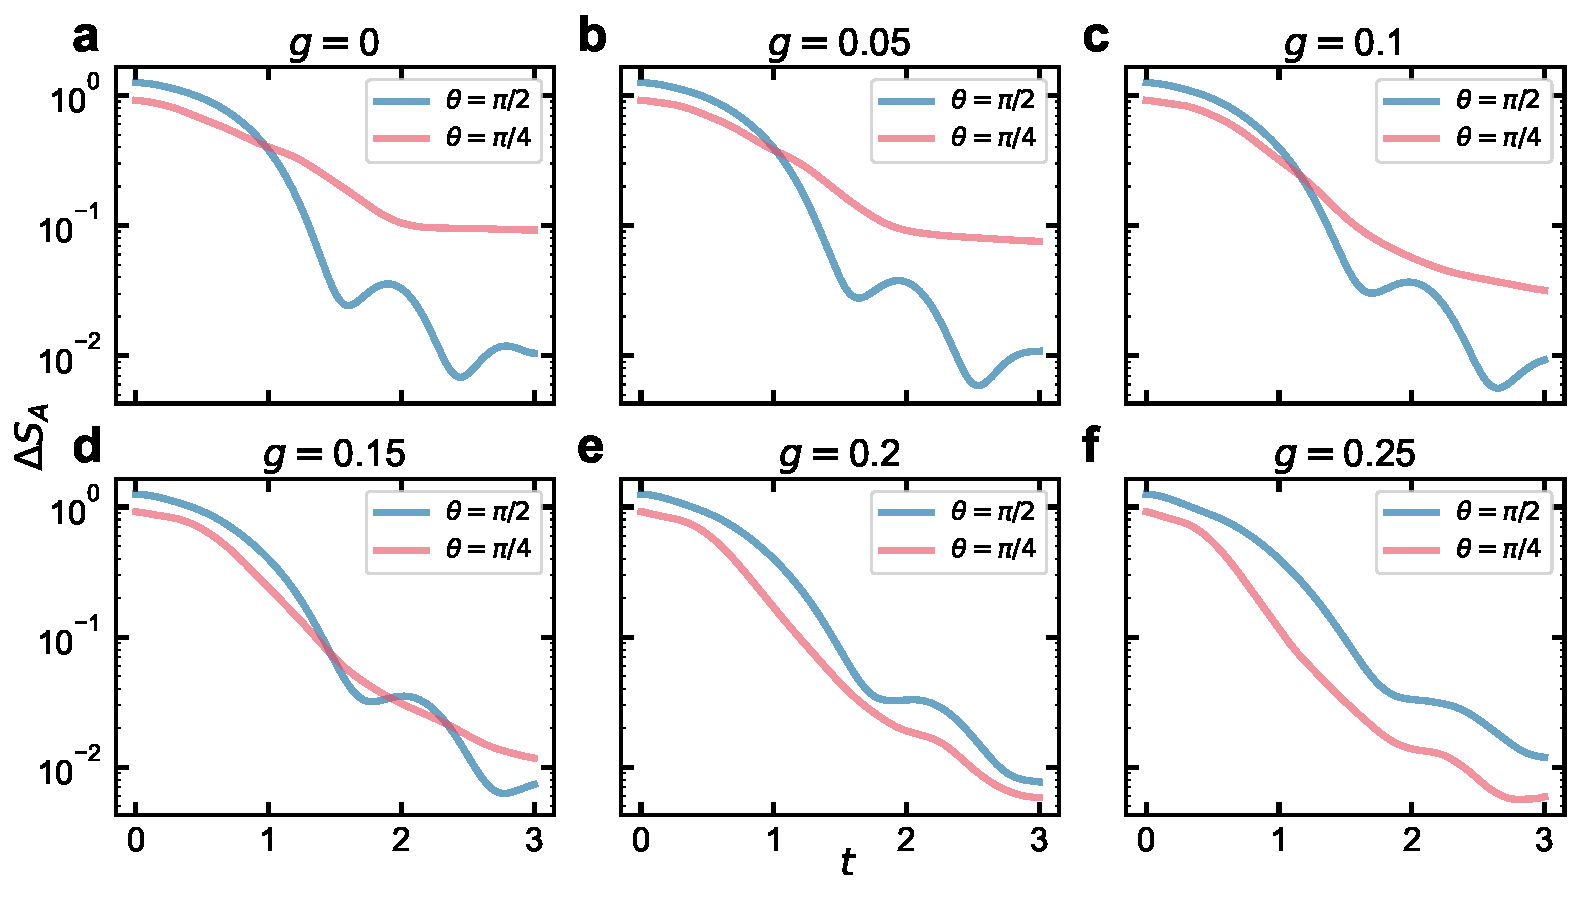
\includegraphics[width=0.9\textwidth]{suppFig/SuppFig1_tunable_r.pdf}
    % \caption{\textbf{EA dynamics at small $r$.}\textbf{a},EA dynamics at $g=0$ when the model is exactly integrable with QME. \textbf{b}-\textbf{d},EA dynamics at $g=0,0.05,0.1,0.15$.When the long range interaction break weakly the integrability, the early dynamics inherit the feature of integrabel case and there also exist QME. \textbf{e}-\textbf{f},EA dynamics at $g=0.2,0.25$. When the long range interaction is strong enough, thermalization even dominates the early dynamics and then there is not QME at all. All simulation is completed in a terminal subsystem [$Q1$,$Q2$,$Q3$] of a open boundary 14 spin chain.}
    \caption{ \textbf{EA dynamics across integrability-breaking regimes.} 
        \textbf{a}, EA dynamics at $g = 0$ (exactly integrable limit), exhibiting the QME. 
        \textbf{b}--\textbf{d}, Weak integrability-breaking regime ($g = 0.05, 0.1, 0.15$): Early-time dynamics retain signatures of integrability, including QME. 
        \textbf{e}--\textbf{f}, Strong integrability-breaking regime ($g = 0.2, 0.25$): Thermalization dominates even at early times, suppressing QME. 
        All simulations are performed for a terminal subsystem [$Q_1$, $Q_2$, $Q_3$] of a 14-spin chain with open boundaries.
    }
    \label{fig:tunable.r}
    \end{figure}
    
    In the integrable limit ($g=0$), the Hamiltonian reduces to an XX spin chain, exactly solvable via Jordan-Wigner transformation to free fermions \cite{introduction_XYchain}. Theoretical studies of EA in such integrable models reveal that QME admits a quasiparticle interpretation: entangled quasiparticle pairs generated within the subsystem contribute to EA, whereas those propagating outside do not. The key insight is that more asymmetric initial states excite faster-propagating modes, accelerating EA decay \cite{NRP2025}. This quasiparticle framework explains observed finite-size oscillations and boundary effects. Furthermore it is consistent with the universal connection between charge distribution and transport modes established by Rylands et al \cite{Integrable_PRL}. Their work demonstrates that more asymmetric states store less charge in slower modes across diverse systems—including free fermions, Rule 54, and the Lieb-Liniger model—with our numerical results aligning precisely with these analytical predictions.
    
    For weak integrability breaking, the Hamiltonian contains perturbations that introduce finite quasiparticle lifetimes. Nevertheless, the early-time dynamics remain consistent with integrable model predictions, as shown in Supplementary Fig.~\ref{fig:tunable.r}. In contrast, when the interaction ratio exceeds, thermalization dominates the dynamics, leading to fundamentally distinct behavior characterized the disappearance of QME signatures. 
    
    \subsection{Analytical result for tilted ferromagnetic state at $r=1$}
    \label{subsec:analytical.result}
    When the interaction ratio $r=1$, the system dynamics admits an exact analytical solution within the collective spin picture. For a system of $N$ spin-$1/2$ qubits, the collective spin operator is defined as:
    \[
    \boldsymbol{S} = \frac{1}{2} \sum_{i=1}^N \boldsymbol{\sigma}^i.
    \]
    The all-to-all XX interaction Hamiltonian transforms to:
    \begin{equation}
    H = g \left( S_x^2 + S_y^2 - \frac{N}{2} \right) = g \left( \boldsymbol{S}^2 - S_z^2 - \frac{N}{2} \right),
    \end{equation}
    where the constant term $-N/2$ contributes only a global phase and thus is negligible. 
    The Hilbert space decomposes into angular momentum sectors with basis states $\ket{S, m}$, where $S$ denotes the total spin quantum number (ranging from $0$ or $1/2$ to $N/2$ for even/odd $N$) and $m$ the magnetic quantum number ($m = -S, \dots, S$). The maximum spin sector $S = N/2$ corresponds precisely to the Fock space, with basis states mapped to computational basis states via:
    \begin{equation}
    \ket{S = \tfrac{N}{2}, m = \tfrac{N}{2} - n} = \frac{1}{\sqrt{\binom{N}{n}}} (\sigma^-)^n \ket{0}^{\otimes N},
    \end{equation}
    where $\binom{N}{n}$ is the binomial coefficient, $\sigma^- = \sum_{i=1}^N \sigma_i^-$ is the collective lowering operator, $\ket{0}^{\otimes N}$ is the all-spin-up state, and $n$ indexes the number of excited qubits ($n = 0, 1, \dots, N$).
    
    The tilted ferromagnetic initial state can be expressed in the following representations:
    \begin{align}
    \ket{\theta}_F &= \left( \cos\frac{\theta}{2} \ket{0} + \sin\frac{\theta}{2} \ket{1} \right)^{\otimes N} \\
    &= \sum_{n=0}^N \left(\cos\frac{\theta}{2}\right)^{N-n}\left(\sin\frac{\theta}{2}\right)^{n} \sqrt{\binom{N}{n}} \ket{S = \tfrac{N}{2}, m = \tfrac{N}{2} - n}.
    \end{align}
    This coherent superposition spans all excitation sectors $n$.
    Under quench dynamics from $\ket{\theta}_F$, $\boldsymbol{S}^2$ becomes conserved, reducing the effective Hamiltonian to the Lipkin-Meshkov-Glick (LMG) model:
    \begin{equation}
    H_{\text{eff}} = -g S_z^2.
    \end{equation}
    The diagonal structure of Hamiltonian yields exact time evolution:
    \begin{equation}
    \ket{\Psi(t)} = e^{-iH_{\text{eff}} t} \ket{\theta}_F = \sum_{n=0}^N \left( \cos\frac{\theta}{2} \right)^{N-n} \left( \sin\frac{\theta}{2} \right)^n \sqrt{\binom{N}{n}} e^{i g t (N/2 - n)^2} \ket{S = \tfrac{N}{2}, m = \tfrac{N}{2} - n}.
    \end{equation}
    Periodic revivals $\ket{\Psi(t = T_S)} \propto \ket{\Psi(0)}$ emerge with revival period:
    \begin{equation}
    T_S = \begin{cases} 
          2\pi/g & \text{even } N \\
          \pi/g & \text{odd } N 
       .\end{cases}
    \end{equation}
    
    \begin{figure}[t]
    \centering
    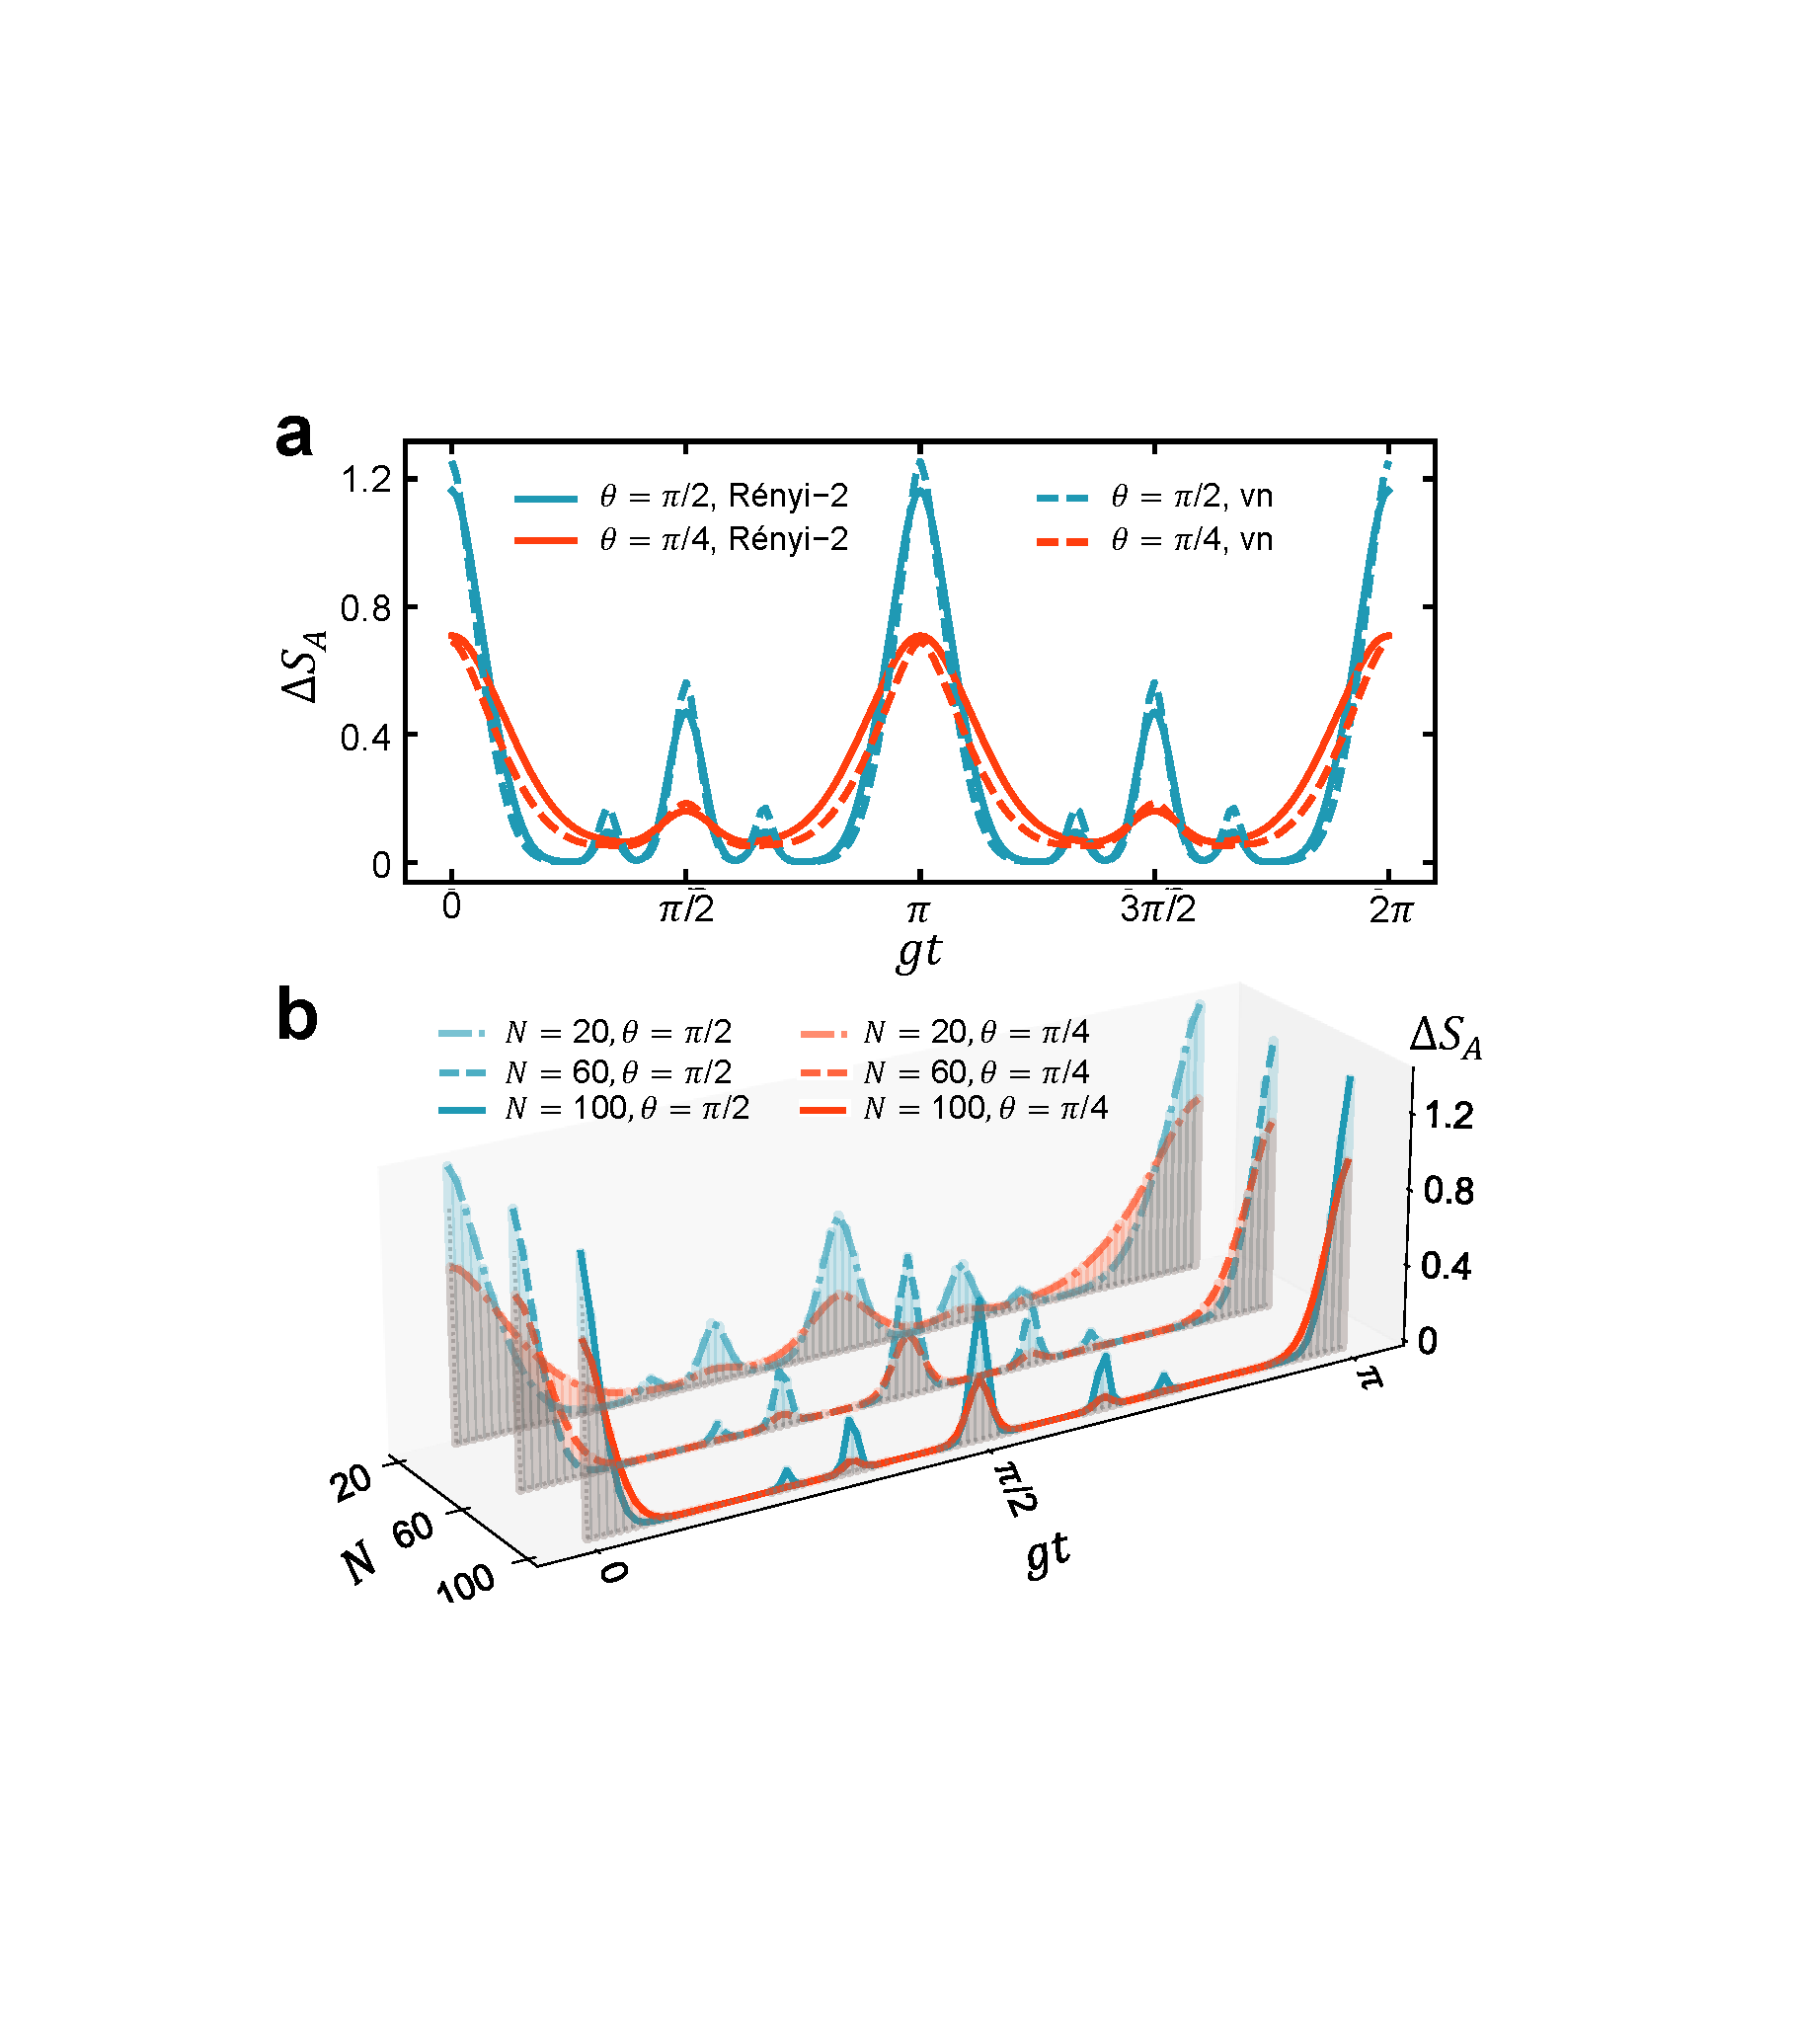
\includegraphics[width=0.6\textwidth]{suppFig/SuppFig2_vn_renyi_tunable_N.pdf}
    \caption{  \textbf{EA dynamics across different measures and system sizes.}
        \textbf{a}, Comparison of EA dynamics using von Neumann entropy and Rényi-2 entropy for subsystem size $N_A = 3$ in a $N = 14$ spin chain. While absolute values differ slightly, both measures capture identical dynamical features.
        \textbf{b}, System-size dependence of EA dynamics (von Neumann entropy) with fixed $N_A = 4$. As $N$ increases, subsystem symmetry restoration accelerates and becomes complete, while the characteristic dynamical crossover preserves.
        }
    % \caption{EA dynamics for fixed $N_A=4$ with varying system sizes $N$.}
    % \textbf{a}, comparison of EA in form of Von-Neumann entropy and Renyi-2 entropy. Despite small difference in value, feature of dynamics keeps similar. $N_A = 3$ and $N=14$. \textbf{b}, EA dynamics for fixed $N_A=4$ with varying system sizes $N$. Along with the increasing system size, the symmetry of subsystem restores faster and fully, while the crossover remains. EA display here is in Von-Neumann entropy. 
    \label{fig:tunable.N}
    \end{figure}
    
    For EA analysis, we partition the total spin $\boldsymbol{S} = \boldsymbol{S}^A + \boldsymbol{S}^{\overline{A}}$ into subsystem $A$ ($N_A$ qubits) and its complement $\overline{A}$, with even $N$ for experimental relevance.
    The Hamiltonian becomes:
    \begin{equation}
    H_{\text{eff}} = -g\left[ (S_z^A)^2 + (S_z^{\overline{A}})^2 + 2 S_z^A S_z^{\overline{A}} \right].
    \end{equation}
    Working in the maximum-spin basis $\ket{S_A = N_A/2, m_1} \otimes \ket{S_{\overline{A}} = (N-N_A)/2, m_2}$,where $m_1$ ranges from $-N_A/2$ to $N_A/2$ and $m_2$ ranges from $-(N-N_A)/2$ to $(N-N_A)/2$,
    subsystem $A$ remains confined to its $S_A = N_A/2$ sector. As a result, $\rho_{A,Q}$ is time-independent, establishing:
    \begin{equation}
    \Delta S_A(t) = C(\theta) - S_A(\theta,t),
    \end{equation}
    with $C(\theta)$ an initial-state-dependent constant,
    \begin{equation}\label{c.theta}
        C(\theta) = -\ln \sum_{n=0}^{N_A} \cos({\theta \over 2})^{4(N_A-n)}\sin({\theta \over 2})^{4n}{\binom{N_A}{n}}^2.
    \end{equation}
    $C(\theta)$ shows a perfect symmetry about $\theta=\pi/2$: it increases monotonically in the interval $(0, \pi/2)$, reaches its maximum at $\theta = \pi/2$, and decreases monotonically in $(\pi/2, \pi)$.
    The time-evolved state is:
    \begin{equation}\label{state.evolution}
    \ket{\Psi(t)} = \sum_{m_1,m_2} C^{N_A}_{m_1}(\theta) C^{N-N_A}_{m_2}(\theta) e^{i g t (m_1 + m_2)^2} \ket{m_1} \otimes \ket{m_2},
    \end{equation}
    with coefficients:
    \begin{equation}
    C^{N}_{m}(\theta) = \left( \cos\frac{\theta}{2} \right)^{N/2 + m} \left( \sin\frac{\theta}{2} \right)^{N/2 - m} \sqrt{\binom{N}{N/2 - m}},
    \end{equation}
    where $\ket{m_1} \equiv \ket{S_A = N_A/2, m_1}$, $\ket{m_2} \equiv \ket{S_{\overline{A}} = (N-N_A)/2, m_2}$. Reduced density matrix elements for subsystem $A$ are:
    \begin{equation}\label{off.diagonal.rho}
    \rho^A_{m_1, m'_1} = C^{N_A}_{m_1}(\theta) C^{N_A}_{m'_1}(\theta) e^{i g t (m_1^2 - m_1'^2)} \sum_{m_2} |C^{N-N_A}_{m_2}(\theta)|^2 e^{2i g t m_2 (m_1 - m'_1)}.
    \end{equation}
    The Rényi-2 EA is:
    \begin{align}
    \Delta S_A &= \ln \left( \frac{\operatorname{Tr}(\rho_A^2)}{\operatorname{Tr}(\rho_{A,Q}^2)} \right) \nonumber \\
    &= \ln \left( 1 + \frac{\sum_{i\neq j}|\rho^A_{i,j}|^2}{\sum_{i}|\rho^A_{i,i}|^2}\right) \\
    &= \ln \left( 1 + \frac{2\sum_{m_1 < m'_1} |C^{N_A}_{m_1}(\theta) C^{N_A}_{m'_1}(\theta)|^2 \mathcal{C}(m_1, m'_1) }{ \sum_{m_1} |C^{N_A}_{m_1}(\theta)|^4 \left( \sum_{m_2} |C^{N-N_A}_{m_2}(\theta)|^2 \right)^2 } \right),
    \end{align}
    where the factor $\mathcal{C}(m_1, m'_1) = \sum_{m_2, m'_2} |C^{N-N_A}_{m_2}(\theta) C^{N-N_A}_{m'_2}(\theta)|^2 \cos[2gt(m_1 - m'_1)(m_2 - m'_2)]$ captures internal coherence of the subsystem. 
    Since $(m_1 - m'_1)$) and $(m_2 - m'_2)$) are integers, EA oscillates with period $T_{\text{EA}} = \pi/g$. At $t = T_{\text{EA}}$:
    \begin{equation}\label{state.pi.2}
    \ket{\Psi(t)} \propto \ket{{-}\theta}_F,
    \end{equation}
    with identical EA to $\ket{\theta}_F$ since $\ket{{-}\theta}_F = e^{-i\pi S_z} \ket{\theta}_F$.
    Although we evaluate EA with Rényi-2 entropy, the dynamics are consistent across different entropy definitions(Fig.~\ref{fig:tunable.N}\textbf{a}). Furthermore, the large system size leads to rapid decay of $\mathcal{C}(m_1, m'_1)$, which accelerates symmetry restoration while maintaining the characteristic crossover behavior (Fig.~\ref{fig:tunable.N}\textbf{b}).
    
    % To visualize the process of symmetry restoration, we admit quasidistribution function,$Q(\theta,\phi) = \langle \theta,\phi | \rho_A | \theta,\phi \rangle$, where $|\theta,\phi\rangle = e^{-i\phi\sum_i \sigma_z^(i)/2} e^{-i\theta\sum_i \sigma_y^(i)/2} |00\cdots0\rangle$ denotes a coherent spin state. At $t=0$, distribution mainly concentrates on the specific direction. During evolution, its distribution along the azimuthal direction becomes uniform, leading to the restoration of $U(1)$ symmetry. The factor that the distribution of $\theta=\pi/2$ flatten faster than that of $\theta=\pi/4$, indicates the QME. At $t=T_{EA}/2$, distribution focus on the two symmetric direction, indicating the $Z2$ symmetry and namely partially $U(1)$ symmetry restoration. In addition, at $t=T_{EA}$, distribution mainly focus on the direction symmetric to that at $t=0$, exhibiting the revival relation $T_S = 2T_{EA}$. Overall, $Q(\theta,\phi)$ provides a clear picture to understand the symmetry restoration for LMG model, which is integrable but not explained by quasiparticle picture.
    
    To visualize the symmetry restoration dynamics, we employ the quasidistribution function $Q(\theta,\phi) = \langle \theta,\phi | \rho_A | \theta,\phi \rangle$, where the coherent spin state is defined as $|\theta,\phi\rangle = e^{-i\phi\sum_i \sigma_z^{(i)}/2} e^{-i\theta\sum_i \sigma_y^{(i)}/2} |00\cdots0\rangle$(see Fig.~\ref{Figure_Qfunction}). Initially ($t=0$), the distribution is sharply peaked along a specific direction. As the system evolves, the azimuthal ($\phi$-direction) distribution gradually becomes uniform, signaling the restoration of $U(1)$ rotational symmetry. The faster flattening of the distribution for $\theta=\pi/2$ compared to $\theta=\pi/4$ directly manifests the QME. At $t=T_{\text{EA}}/2$, the distribution bifurcates into two symmetric peaks, revealing emergent $Z_2$ symmetry and partial $U(1)$ symmetry restoration. By $t=T_{\text{EA}}$, the distribution revives to a configuration symmetric to the initial state, demonstrating the relation $T_S = 2T_{\text{EA}}$.
    Crucially, these $Q(\theta,\phi)$ dynamics provide a complete visualization of symmetry restoration in the integrable LMG model—a process that cannot be explained through conventional quasiparticle propagation.
    
\begin{figure}[t]
    \centering
    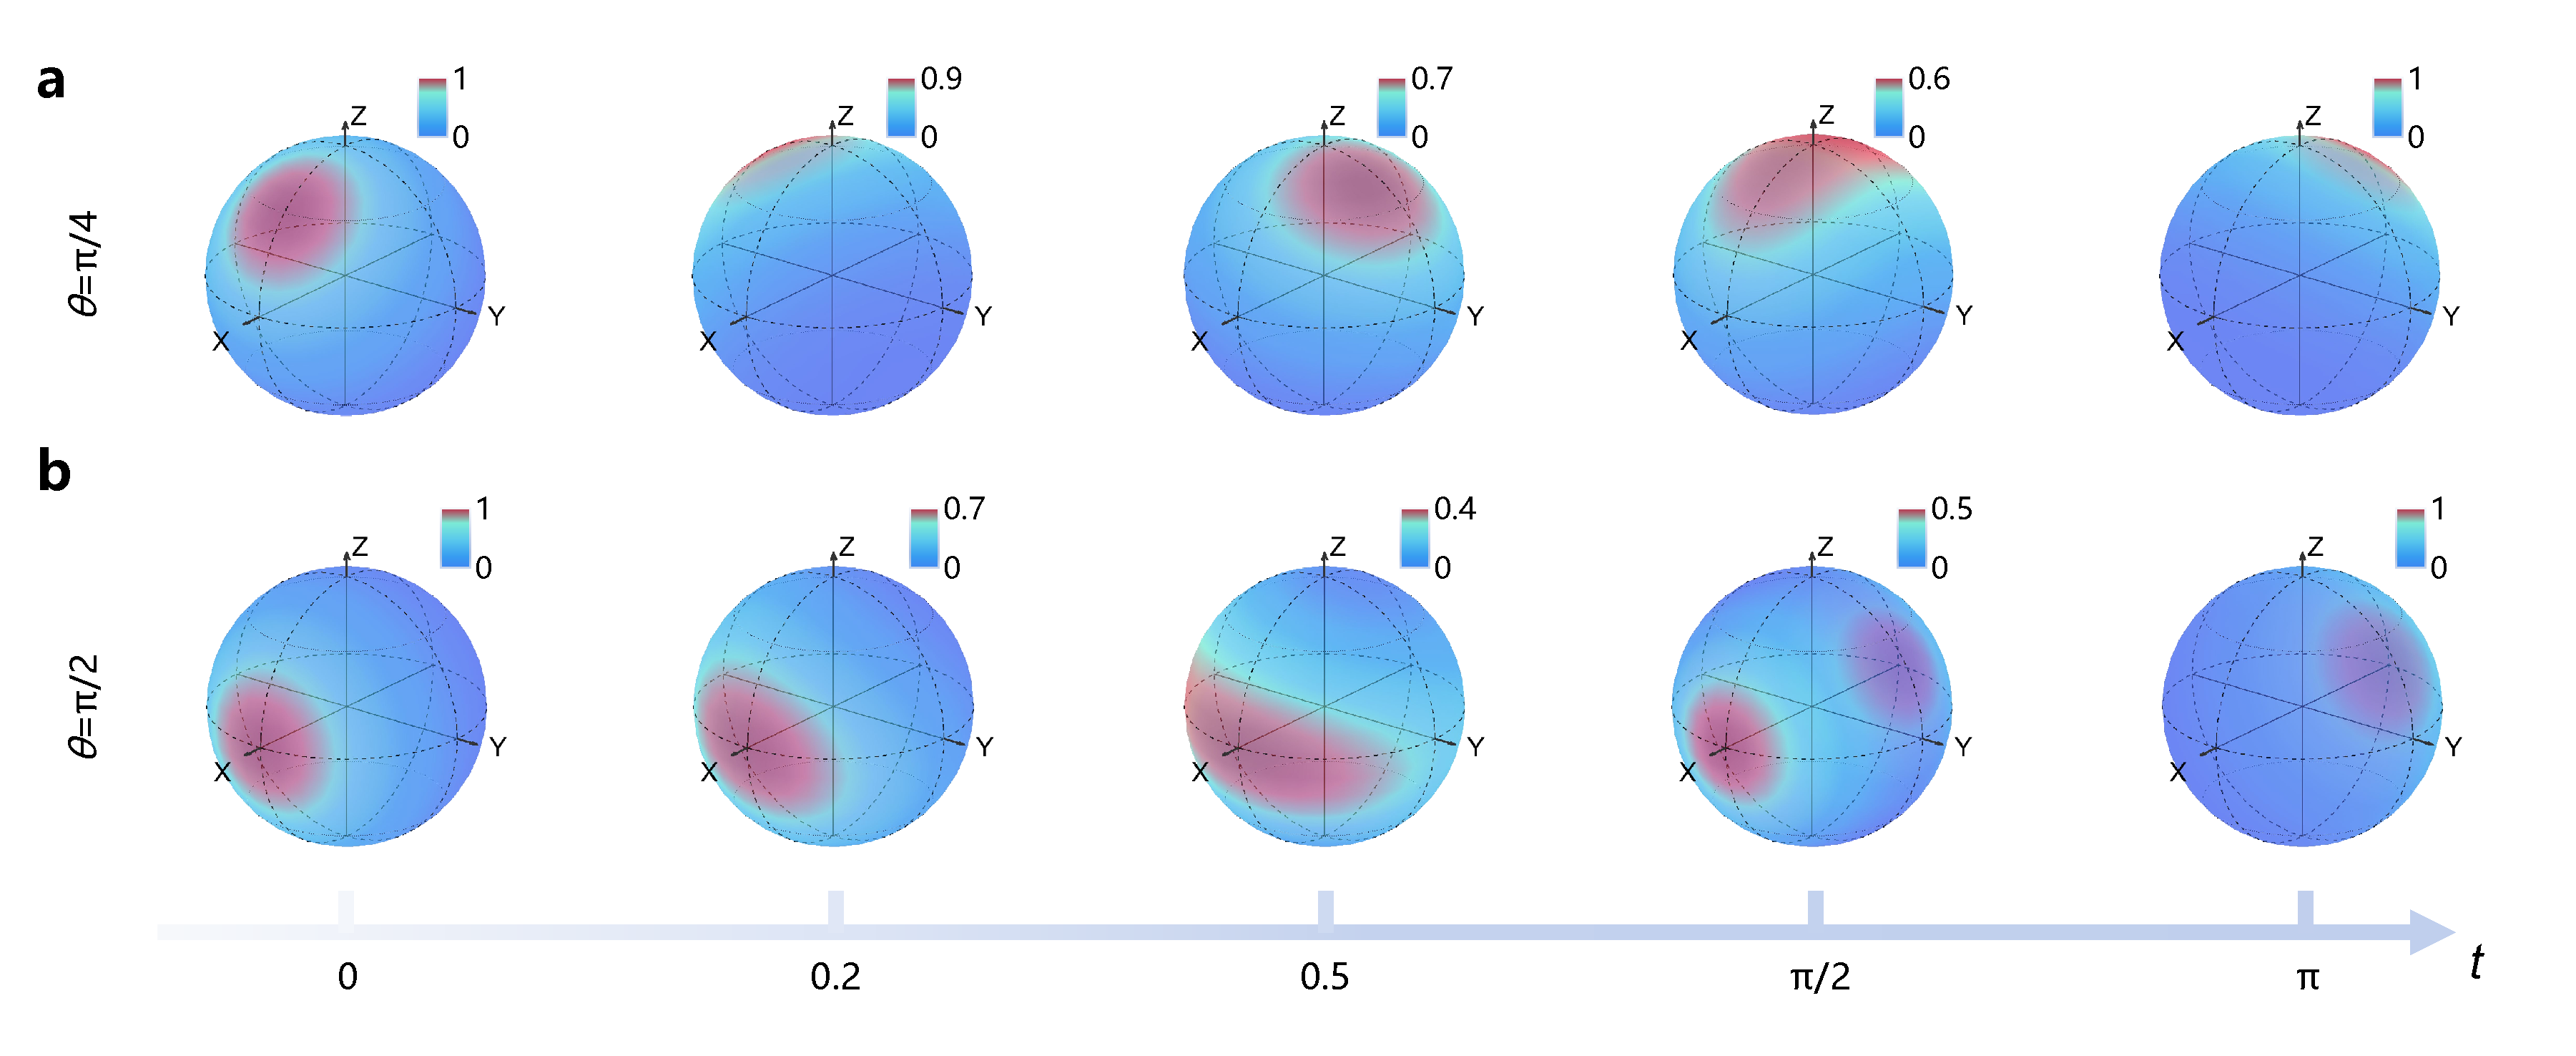
\includegraphics[width=1.0\textwidth]{suppFig/Figure_Qfunction.pdf}
    \caption{
        \textbf{Dynamics of the quasidistribution function.} 
        (a) $\theta = \pi/4$ and (b) $\theta = \pi/2$ evolution. The azimuthal distribution evolves toward uniformity, reflecting $U(1)$ symmetry restoration. Notably, faster flattening at $\theta = \pi/2$ (vs. $\pi/4$) demonstrates the QME. Key features include: (i) $Z_2$-symmetric bifurcation at $t = T_{\text{EA}}/2$ (partial $U(1)$ restoration), and (ii) full revival at twice the EA period ($T_S = 2T_{\text{EA}}$) as the distribution returns to a configuration symmetric to the initial state. System size $N=14$ and $N_A=3$, matching experimental setup.}
    \label{Figure_Qfunction}
\end{figure}

    
    \subsection{Effect of onsite potential on EA dynamics}
    
    Our work further investigates the relationship between onsite potentials and the QME, examining linear potential effects on tilted N\'eel states and disorder effects on tilted ferromagnetic states in the $r\approx 1$ regime.

    In the absence of onsite potentials, symmetry restoration occurs faster for tilted N\'eel states with smaller tilt angles, thereby suppressing QME. This behavior is corroborated by entanglement dynamics measurements (see Fig.~\ref{fig3}\textbf{a}), where the entanglement entropy increases linearly and then saturate. 
    Given the small energy difference of tilted N\'eel states ($\langle H \rangle / (e_{\text{max}} - e_{\text{min}}) = 0.03$ for $\theta = \pi/4$ versus $0.06$ for $\theta=\pi/2$, where $e_{\text{max}}$ and $e_{\text{min}}$ denote the maximal and minimal eigenenergies of the system respectively), both states naturally evolve toward the same steady state, with their EE saturating at the Page value.
    In this case, EE serve as the indicator of thermalizaiton rate. The temporal evolution of EE closely mirrors EA dynamics, confirming that states thermalizing faster restore symmetry more rapidly. This correlation originates from thermalization driving the system toward a $U(1)$-symmetric thermal Gibbs ensemble, intrinsically linking thermalization to symmetry restoration.
    
    \begin{figure}[t]
    \centering
    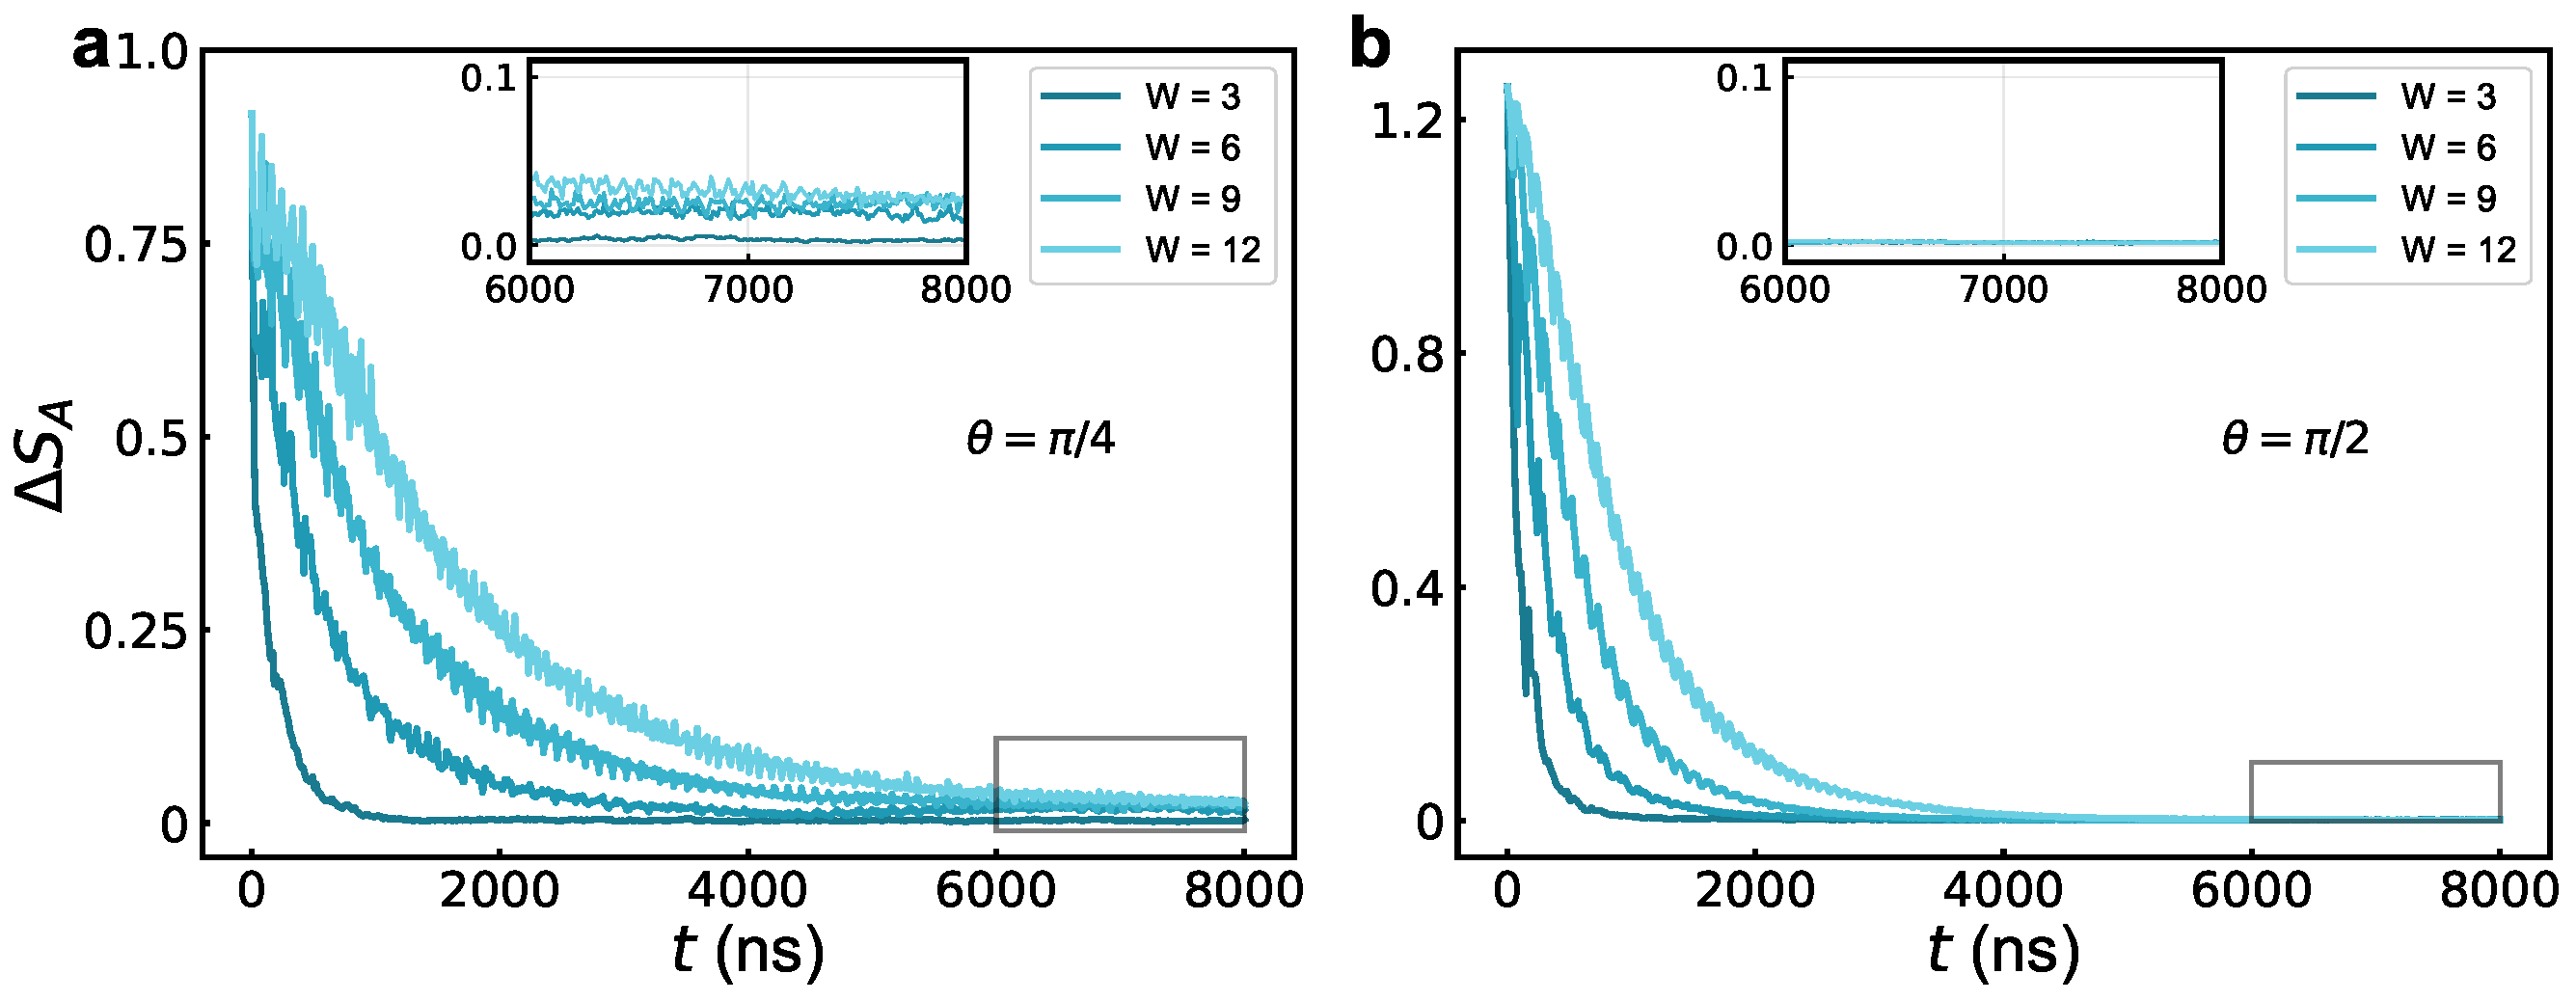
\includegraphics[width=0.9\textwidth]{suppFig/SuppFig4_EA_W_longtime.pdf}

    \caption{  \textbf{EA dynamics across potential strength.} 
        \textbf{a}, For $\theta = \pi/4$, EA decays from its initial value to a small but finite late-time plateau, whose magnitude grows systematically with $W =3,6,9,12$ MHz within the simulated range. 
        \textbf{b}, For $\theta = \pi/2$, EA decays to near zero ($\Delta S_A \simeq 0$) for all tested $W$ values. 
        This $\theta$ dependence of the response of EA to the linear potential underlies the QME reemergence.
    }
    \label{fig:longtime.EA.W}
    \end{figure}
    
    Under strong linear potentials, although symmetry restoration generally slows down, the degree of suppression depends on tilt angle $\theta$ - states with larger $\theta$ show less suppression and thus the QME recovers.
    As shown in Fig.~\ref{fig:longtime.EA.W}, numerical simulations of long-time behavior across potential strengths $W$  reveal that $\Delta S_A(t\rightarrow \infty)$ remains nearly constant for $\theta=\pi/2$ but increases for $\theta=\pi/4$ within the studied range, satisfying:
    \begin{align}
    \Delta S_A(\pi/4,t=0) &< \Delta S_A(\pi/2,t=0) \\
    \Delta S_A(\pi/4,t\to\infty) &> \Delta S_A(\pi/2,t\to\infty)
    \end{align}
    We attribute this phenomenon to potential-induced ergodicity breaking. 
    Supporting evidence comes from two key observations:
    (i) The mean energy-level spacing ratio approaches the Poisson limit ($\langle r \rangle \to 0.386$), calculated as
    \begin{equation}
    \expval{r} = \frac{1}{N} \sum_{n=1}^N \frac{\min(\delta_n, \delta_{n+1})}{\max(\delta_n, \delta_{n+1})},
    \end{equation}
    where $\delta_n = E_n - E_{n-1} $ denotes the adjacent eigenenergy gap (Fig.~\ref{fig:r.Imbalance}\textbf{a}).
    (ii) The imbalance exhibits persistent non-zero values with increasing potential strength $W$ (Fig.~\ref{fig:r.Imbalance}\textbf{b}).
    
    \begin{figure}[t]
    \centering
    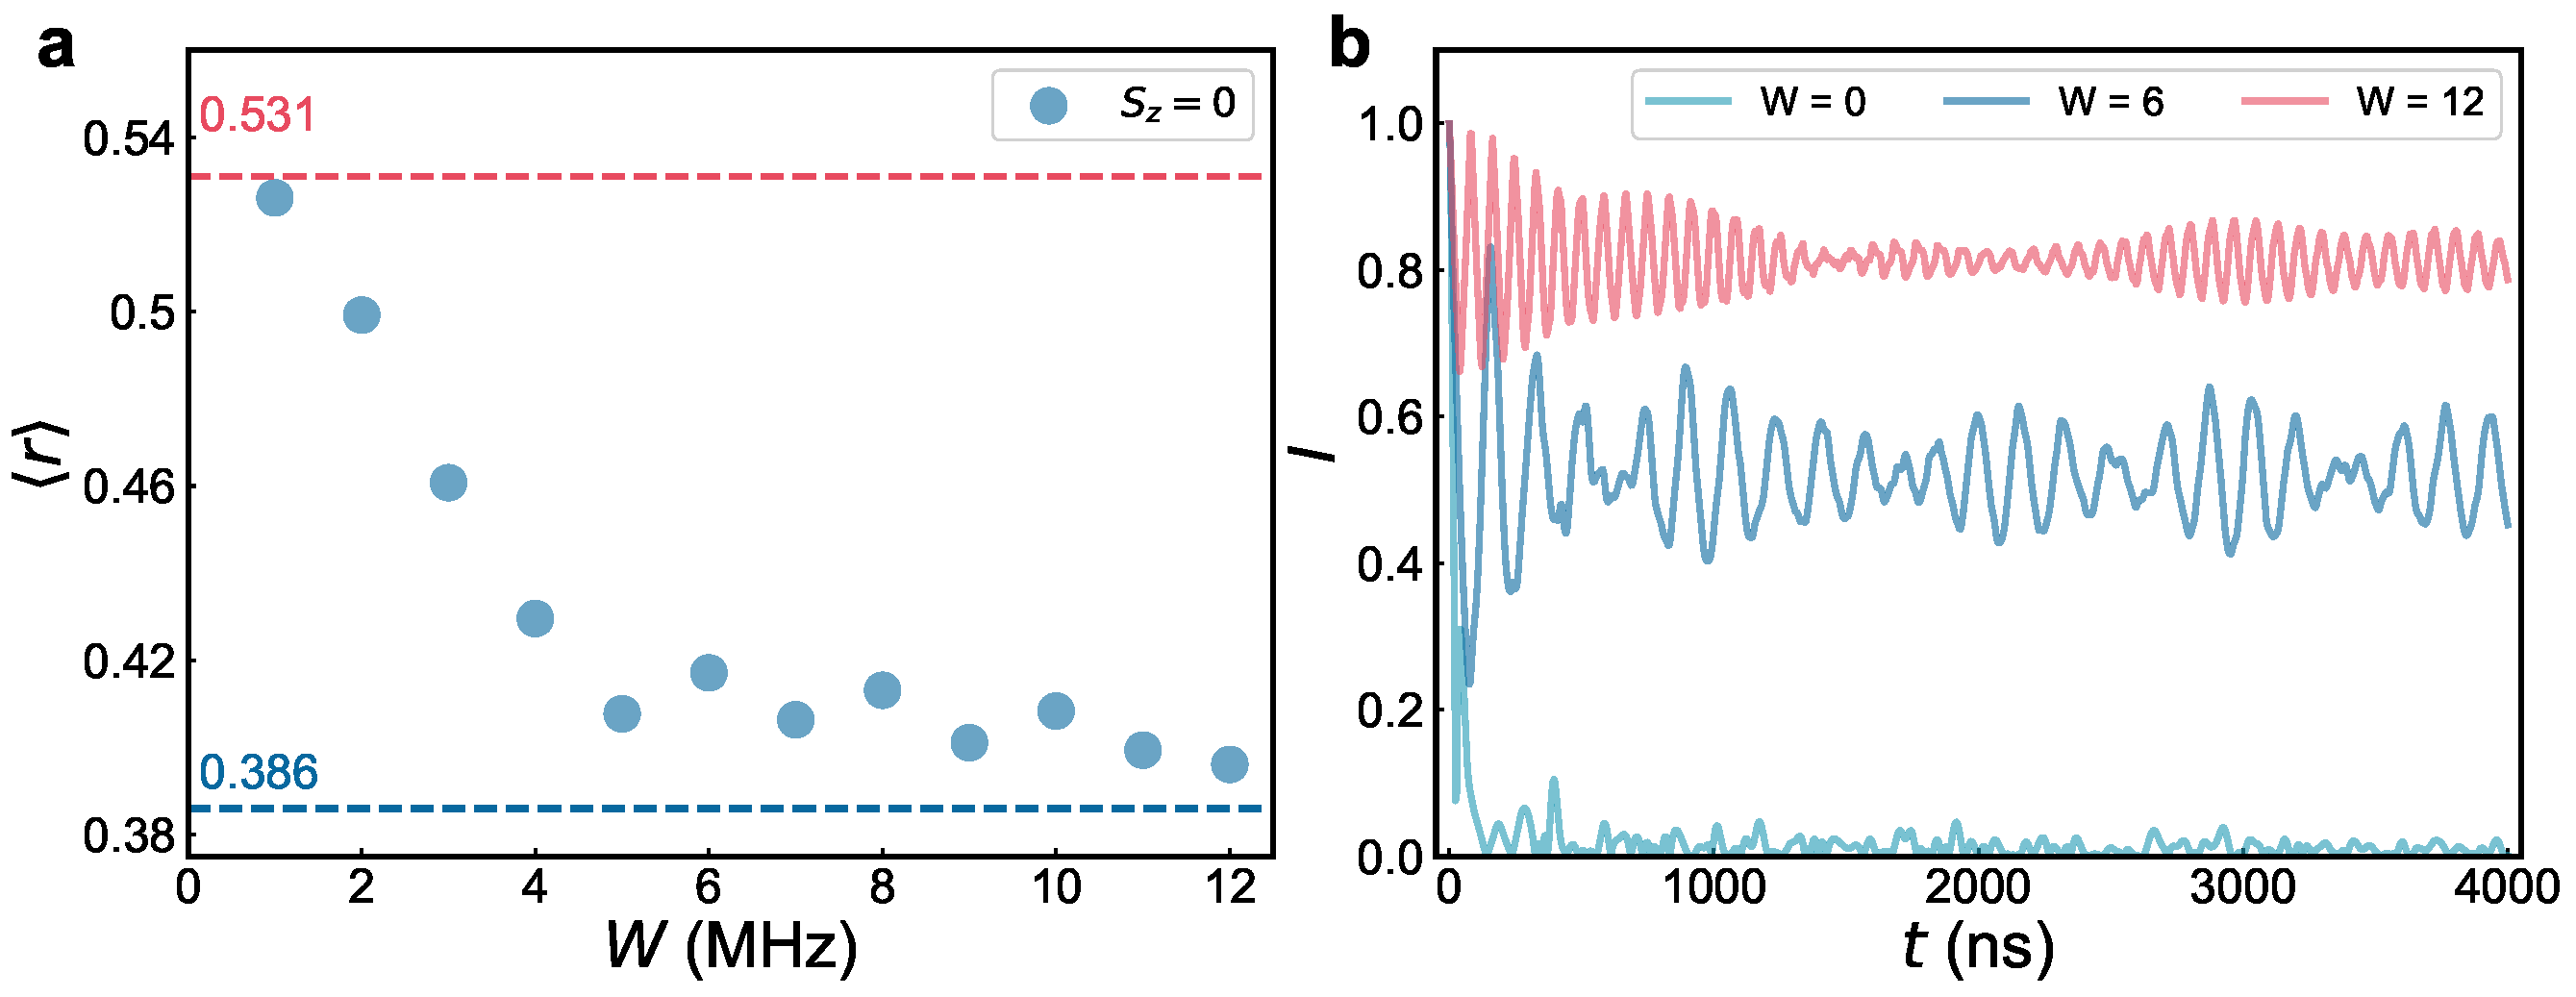
\includegraphics[width=0.9\textwidth]{suppFig/SuppFig5_r_Imbalance.pdf}
    \caption{
        \textbf{Indicators of ergodicity breaking under linear potential.} 
        \textbf{a}, The mean energy-level spacing ratio $\langle r \rangle$ in the $S_z=0$ subspace versus potential strength $W$. The approach of $\langle r \rangle$ to $0.386$ at large $W$ signals the onset of ergodicity breaking, consistent with Poisson statistics. 
        \textbf{b}, Imbalance dynamics for $W=6,12$ MHz shows persistent oscillations around finite values, providing complementary evidence of non-ergodic behavior.
    }
    \label{fig:r.Imbalance}
    \end{figure}
    
    For tilted ferromagnetic states, QME persists in the disorder-free case and demonstrates exceptional robustness against studied disorder strengths $ h_i \in [-\delta_z,\delta_z]\bar{g}$ with $\delta_z = 7,14,21$. As shown in Fig.~\ref{Disorder_ferr}, the characteristic EA crossover persists despite strong disorder.

    
    \begin{figure}[h]
    \centering
    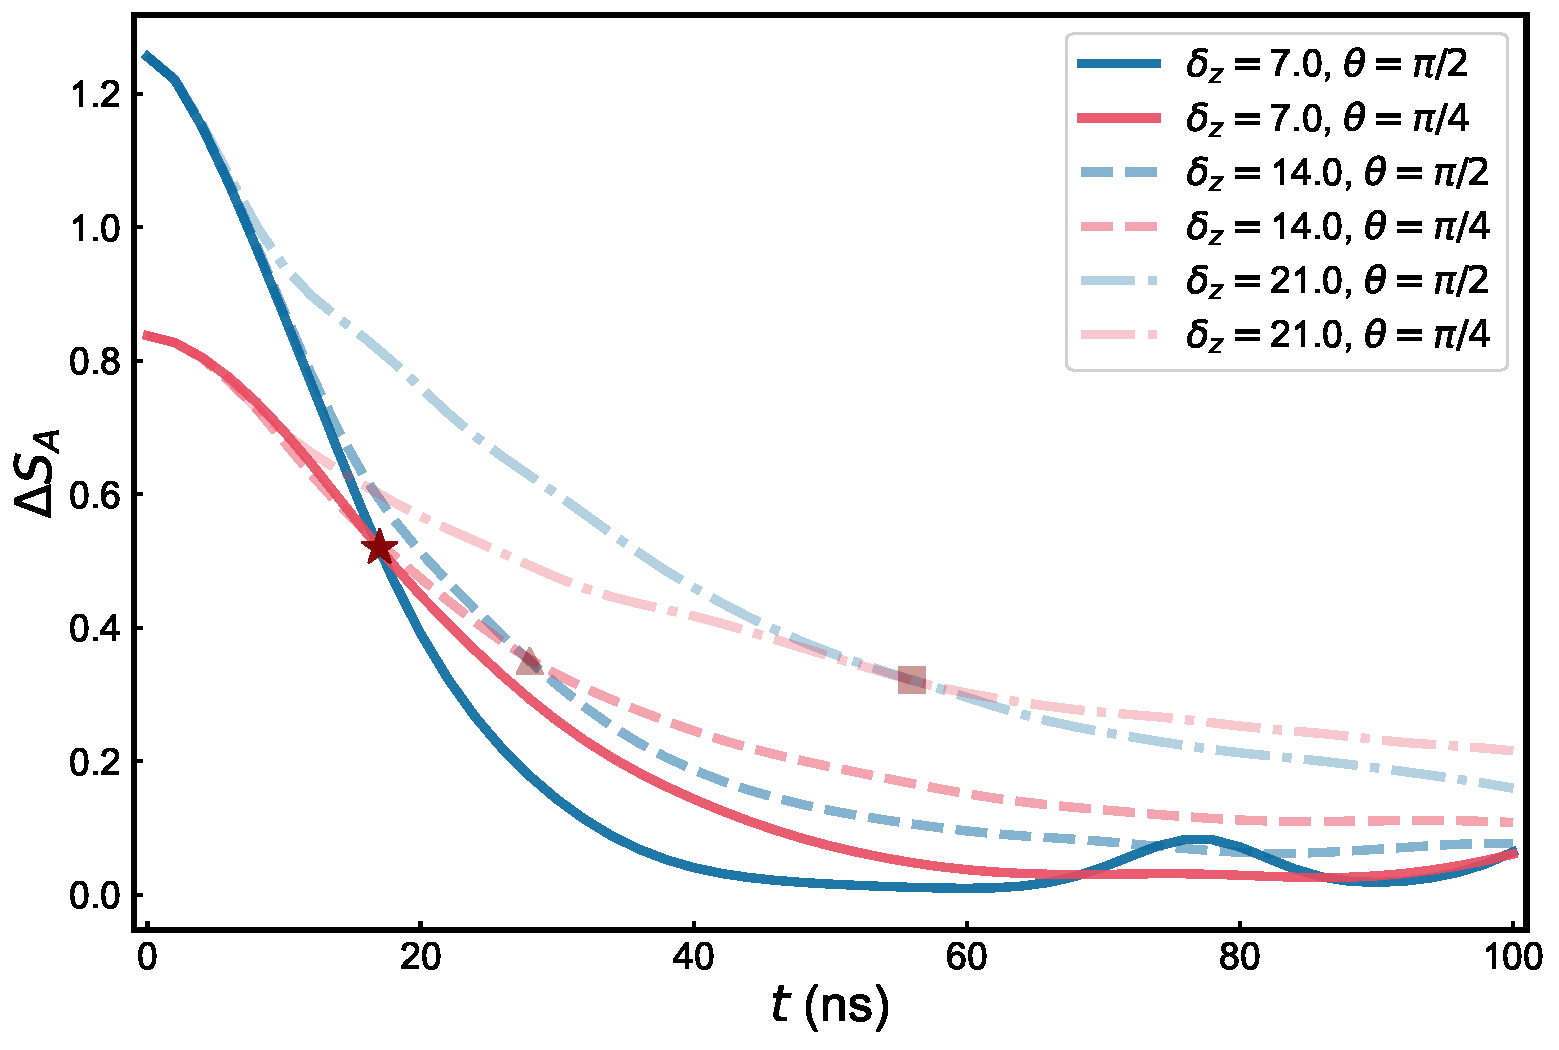
\includegraphics[width=0.7\textwidth]{suppFig/SuppFig6_EA_disorder.pdf}
    \caption{ \textbf{Disorder-dependent EA dynamics for tilted ferromagnetic state.} 
        Increasing the onsite disorder strength $\delta_z $ systematically slows both the symmetry restoration and dynamical crossover of EA, yet all crossover remain below 100 ns. Simulations employ experimental parameters with disorder fields $h_i \in [-\delta_z,\delta_z]\bar{g}$ sampled from a uniform distribution, averaging over 100 disorder realizations for statistical convergence.
    }
    \label{Disorder_ferr}
    \end{figure}
	 
	 \subsection{Decoherence Effects and Simulation Methodology}
	 
	Experimental decoherence influences EA dynamics. Prior studies demonstrate that while decoherence accelerates symmetry restoration, it cannot by itself generate the QME~\cite{QME_trapped_ion}. Crucially, our results—together with those in Ref.~\cite{QME_trapped_ion}—reveal the robustness of QME under realistic decoherence conditions.
	 
    Accurate simulation of experimental EA dynamics requires incorporating decoherence through the Lindblad master equation. The conventional Liouville operator approach faces computational limitations, with memory requirements scaling as $\mathcal{O}(2^{4N})$ for an $N$-qubit system, becoming prohibitively expensive for large systems.
    
    The quantum trajectory method provides an efficient alternative, trading memory resources for computational time. This technique simulates continuous quantum measurements through infinitesimal time steps $dt$. At each step, the measurement outcome is:
    \begin{equation}
    dy = \langle X \rangle dt + \frac{dW}{\sqrt{8\kappa}},
    \end{equation}
    where $X$ is the measurement operator and $dW$ represents Wiener noise satisfying:
    \begin{equation}
    \mathbb{E}[dW] = 0, \quad \operatorname{Var}[dW] = dt.
    \end{equation}
    State evolution follows the stochastic Schrödinger equation:
    \begin{equation}
    d\ket{\psi} = \left[ -iH dt -\kappa(X-\langle X\rangle)^2 dt + \sqrt{2\kappa}(X-\langle X \rangle)dW \right] \ket{\psi(t)}.
    \end{equation}
    Equivalently, the density matrix evolves according to the stochastic master equation:
    \begin{equation}
    d\rho = -i [H,\rho]dt -\kappa[X,[X,\rho]]dt + \sqrt{2\kappa}\left( X\rho + \rho X - 2\langle X \rangle\rho \right)dW.
    \end{equation}
    Remarkably, averaging over $M$ trajectories recovers the exact Lindblad dynamics:
    \begin{equation}
    d\bar{\rho} = -i [H,\bar{\rho}]dt -\kappa[X,[X,\bar{\rho}]]dt,
    \end{equation}
    where $\bar{\rho}(t) = \frac{1}{M}\sum_{i=1}^M \rho_i(t)$. This equivalence transforms the memory requirement from $\mathcal{O}(2^{4N})$ to $\mathcal{O}(2^{N})$ state-vector simulations at the cost of $M/dt$ time steps, effectively converting memory constraints into computational time.
    
    Optimal implementation of the quantum trajectory method requires balancing the time-step size \( dt \) and the trajectory count \( M \). We validate this method against exact Lindblad solutions for systems with \( N = 10 \) qubits, as shown in Supplementary Fig.~\ref{state_traj}a, demonstrating that as the trajectory count \( M \) increases, the results converge to exact Lindblad solutions. Supplementary Fig.~\ref{state_traj}b further shows the convergence of EA dynamics with increasing \( M \) under experimental parameters. These results confirm that with sufficient trajectories and appropriate time discretization, the quantum trajectory method reliably approximates Lindblad evolution for large-scale quantum systems. The simulation results in the main manuscript were obtained via the quantum trajectory method, using a time step of \( dt = 0.15 \) and \( M = 100 \) trajectories.
    
    \begin{figure}[h]
    \centering
    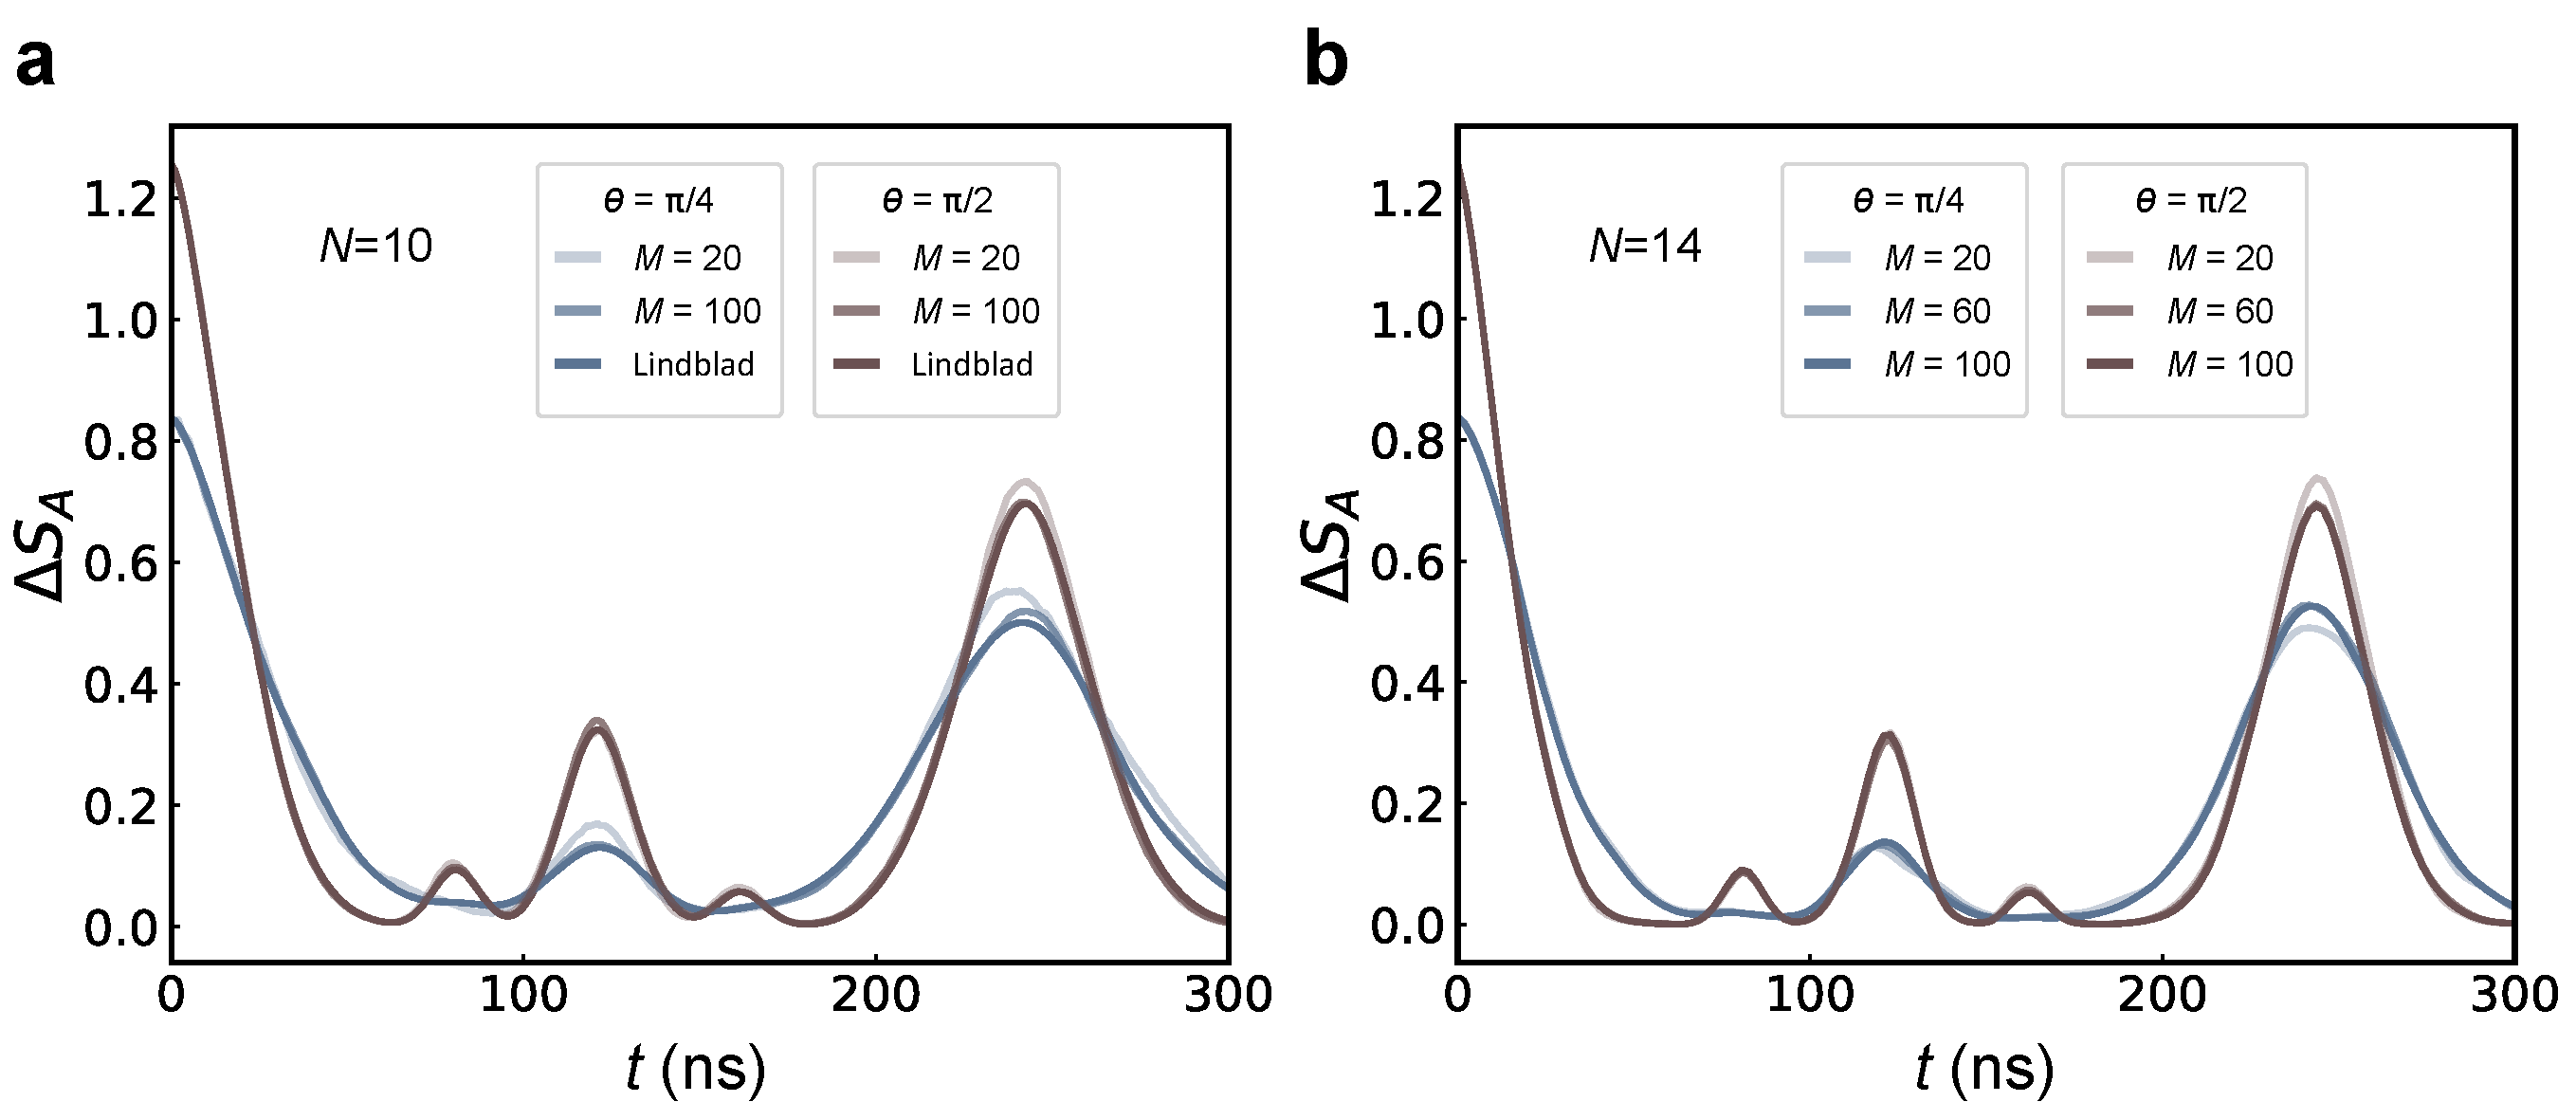
\includegraphics[width=0.95\textwidth]{suppFig/plot_state_traj.pdf}
    \caption{\textbf{Verification of EA dynamics for the tilted ferromagnetic state using the quantum trajectory method.} \textbf{a}, For a small system (\( N = 10 \)), the results approach those obtained from exact solutions of the Lindblad equation as the trajectory count \( M \) increases. \textbf{b}, The results gradually converge with increasing trajectory count \( M \). All results obtain through quantum trajectory method using \( \mathrm{d}t = 0.15 \).}
    
    \label{state_traj}
    \end{figure}
    
% 	\clearpage
% 	\newpage

    

%
% ****** End of file apssamp.tex ******
	
\end{document}